\section{Abstract}\label{abstract}

AI systems can now generate plans, code, analyses, and tool actions at
high speed. Institutions need something harder: evidence that binds an
objective to an execution, an execution to a trace, a trace to
independent evaluation, evaluation to challenge rights, and any
consequential decision to explicit authority. This paper presents GoalOS
AGIALPHA Ascension Sovereign Machine Economy Kernel v3, a constitutional
execution substrate for proof-bearing autonomous work.

The architecture integrates three complementary engines. META-AGENTIC
α-AGI forms and charters bounded agent institutions. AGI Alpha Node v0
admits resources, executes bounded work, and emits evidence-bearing
receipts. AGI Jobs v0 (v2) convenes work markets, preserves independent
validation and dissent, and prepares non-live settlement intent. Kernel
v3 sits beneath these engines as the proof-to-permission boundary: a
DOM-independent 17-state machine, ten typed protocol envelopes, five
role-separated Ed25519 signing authorities, a Web Worker-owned
transition path, an append-only IndexedDB Chronicle, portable mission
bundles, independent replay verification, and signed Human Review
Certificates.

The system introduces an end-to-end operating doctrine - Identify,
Out-Learn, Out-Think, Out-Design, Out-Strategise, Out-Execute - while
preserving a strict invariant: evidence completion is not factual
certification, signatures are not identity proof, and human review
records scope without itself triggering external execution. The
reference release is browser-local and default-deny: it makes no network
requests, connects no wallet, moves no token, calls no live model, and
grants no external authority. The contribution is architectural and
falsifiable. We define the object model, state-transition law, evidence
semantics, authority matrix, threat model, conformance levels, benchmark
program, deployment doctrine, and autonomous publication law required to
turn AI output into governed, auditable, reusable institutional
capability.

This edition adds a qualification frontier, ten quintessential
institutional use cases, seven worked reference case studies, and a
reusable case-study dossier standard. Each scenario is explicit about
evidence status, human authority, rollback, success metrics, and
falsification. The purpose is not to imply deployment; it is to show how
the kernel becomes useful in boardrooms, operating environments,
regulated workflows, scientific programs, and machine-labor markets.

Keywords: autonomous AI work; proof-to-permission; constitutional state
machine; Evidence Docket; human review; agent institutions; verifiable
execution; machine economy; event Chronicle; typed envelopes; Ed25519;
GoalOS.

\section{Executive thesis}\label{executive-thesis}

A model can answer. An agent can act. An institution must prove.

The first age of generative AI made output abundant. The next
institutional bottleneck is not output. It is the ability to decide
which output deserves trust, propagation, reuse, settlement, and
permission. GoalOS Mission OS defined the user-facing product as an
objective-to-proof system whose deliverable is a Governed Decision State
rather than a report {[}1{]}. AGI ALPHA defined the organizational
substrate above models: agents, jobs, validators, tools, memory,
markets, settlement, governance, and capacity allocation {[}2{]}.
AEP-001 defined the constitutional law of evolution: Aim -\textgreater{}
Act -\textgreater{} Prove -\textgreater{} Evolve, with proof-carrying
artifacts, hard selection gates, public-private boundaries, and rollback
{[}3{]}.

Kernel v3 is the executable synthesis of those ideas. It does not
attempt to make a model omniscient or an agent sovereign. It makes
institutional reliance explicit. A mission is committed. An institution
is chartered. A node is admitted. Work is bounded. Evidence is sealed.
Validation is separated from execution. Dissent and challenge remain
visible. Settlement intent remains non-live. Human review records scope,
expiry, unresolved risks, and revocation. Memory is promoted only as a
reversible candidate.

\begin{longtable}[]{@{}
  >{\raggedright\arraybackslash}p{(\columnwidth - 0\tabcolsep) * \real{1.0000}}@{}}
\toprule\noalign{}
\begin{minipage}[b]{\linewidth}\raggedright
\textbf{InstitutionalWork = Output × Proof × Validation × Authority ×
Rollback × Reuse}

(1)
\end{minipage} \\
\midrule\noalign{}
\endhead
\bottomrule\noalign{}
\endlastfoot
\end{longtable}

If proof, validation, authority, or rollback readiness is zero, the
system may still have generated output, but it has not produced trusted
institutional work. This distinction is the heart of the paper.

\begin{longtable}[]{@{}
  >{\raggedright\arraybackslash}p{(\columnwidth - 0\tabcolsep) * \real{1.0000}}@{}}
\toprule\noalign{}
\begin{minipage}[b]{\linewidth}\raggedright
\textbf{Canonical doctrine.}

AI creates output. GoalOS creates proof. No proof, no evolution. No
eval, no propagation. No rollback, no release. Replace the intelligence,
never the constitution.
\end{minipage} \\
\midrule\noalign{}
\endhead
\bottomrule\noalign{}
\endlastfoot
\end{longtable}

\section{Reader map}\label{reader-map}

\begin{longtable}[]{@{}
  >{\raggedright\arraybackslash}p{(\columnwidth - 4\tabcolsep) * \real{0.3333}}
  >{\raggedright\arraybackslash}p{(\columnwidth - 4\tabcolsep) * \real{0.3333}}
  >{\raggedright\arraybackslash}p{(\columnwidth - 4\tabcolsep) * \real{0.3333}}@{}}
\toprule\noalign{}
\begin{minipage}[b]{\linewidth}\raggedright
\textbf{Reader}
\end{minipage} & \begin{minipage}[b]{\linewidth}\raggedright
\textbf{Primary question}
\end{minipage} & \begin{minipage}[b]{\linewidth}\raggedright
\textbf{Recommended sections}
\end{minipage} \\
\midrule\noalign{}
\endhead
\bottomrule\noalign{}
\endlastfoot
\textbf{Executive / investor} & What category is being created, and why
might it matter? & 1-4, 15-21, 24 and Conclusion \\
\textbf{Enterprise operator} & How does an objective become a governed
decision and bounded action? & 4-6, 10-12, 16-21 \\
\textbf{Protocol engineer} & What are the state machine, envelopes,
signatures, Chronicle, and adapters? & 5-11, 20-22 and Appendices A-C \\
\textbf{Risk / governance} & Where does authority sit, how does the
system fail closed, and what is not claimed? & 7, 10-14, 16, 20-23 \\
\textbf{Evaluator / auditor} & What evidence is produced, how is it
replayed, and what would falsify the thesis? & 9-14, 17-18, 20-23 \\
\textbf{Researcher} & What is novel relative to Mission OS, AGI ALPHA,
AEP-001, and proof-carrying systems? & 2-5, 13-14, 17-18, 20-21 \\
\textbf{Board / procurement / policy} & Which missions merit proof-gated
autonomy, and what should human reviewers receive? & 20-21 and
Appendices F-G \\
\end{longtable}

\section{Canonical contributions}\label{canonical-contributions}

\begin{enumerate}
\def\labelenumi{\arabic{enumi}.}
\item
  An executable proof-to-permission kernel that separates intelligence
  from authority and state advancement from interface behavior.
\item
  A three-engine institutional architecture: META-AGENTIC institution
  formation, AGI Alpha Node bounded execution, and AGI Jobs proof-gated
  market coordination.
\item
  A 17-state constitutional lifecycle with transition-specific issuers,
  hard guards, fail-closed terminal states, and a distinct human review
  boundary.
\item
  Ten typed protocol envelopes that bind purpose, issuer, predecessor,
  payload commitment, logical time, scope, and signature.
\item
  Five signing authorities that prevent one actor from proposing,
  executing, validating, settling, and authorizing the same work.
\item
  An append-only Chronicle and portable mission-bundle format that
  support strict replay, import quarantine, tamper detection, and
  revocable memory.
\item
  A replaceable six-method adapter contract that allows models,
  enterprise systems, evaluators, and contract interfaces to change
  without weakening governance.
\item
  A Human Review Certificate that records disposition, scope, expiry,
  unresolved risk, settlement posture, memory disposition, and
  revocation rights without triggering external action.
\item
  An autonomous publication law that applies the same constitutional
  discipline to the public website: source, deterministic build, QA,
  pull request, human review, and deployment.
\item
  A falsifiable benchmark and conformance program that measures proof
  integrity, false permission, replay, challengeability, proof debt,
  verified work density, reuse, and governance overhead.
\item
  An institutional use-case and case-study framework that qualifies
  missions by consequence and evidence burden, then converts each
  scenario into a mission contract, typed state path, Evidence Docket,
  Human Review Certificate, and revocable capability package.
\end{enumerate}

\section{1. From output to
proof-to-permission}\label{from-output-to-proof-to-permission}

Large models have made generation cheap. Agent frameworks have made tool
use and multi-step execution increasingly accessible. Neither
development, by itself, makes organizational reliance cheap.
Institutions must answer questions that ordinary prompt-response systems
leave implicit: What exactly was authorized? Which sources support each
claim? Which assumptions remain unresolved? Which actor performed which
step? What failed? Which validator was independent? What can be
challenged? What may be reused? What is reversible? Who can authorize
consequence?

GoalOS Mission OS addressed the product gap by defining a Governed
Decision State: mission contract, claims matrix, source provenance,
contradiction register, Evidence Docket, verifier report, risk ledger,
executive brief, action graph, Chronicle entry, and reusable capability
package {[}1{]}. AGI ALPHA addressed the organizational gap by treating
intelligence as governed machine labor across agents, jobs, validators,
tools, memory, markets, settlement, and governance {[}2{]}. AEP-001
addressed the evolutionary gap by requiring proof, evaluation, scope,
canary control, challenge windows, and rollback before an artifact may
influence future work {[}3{]}.

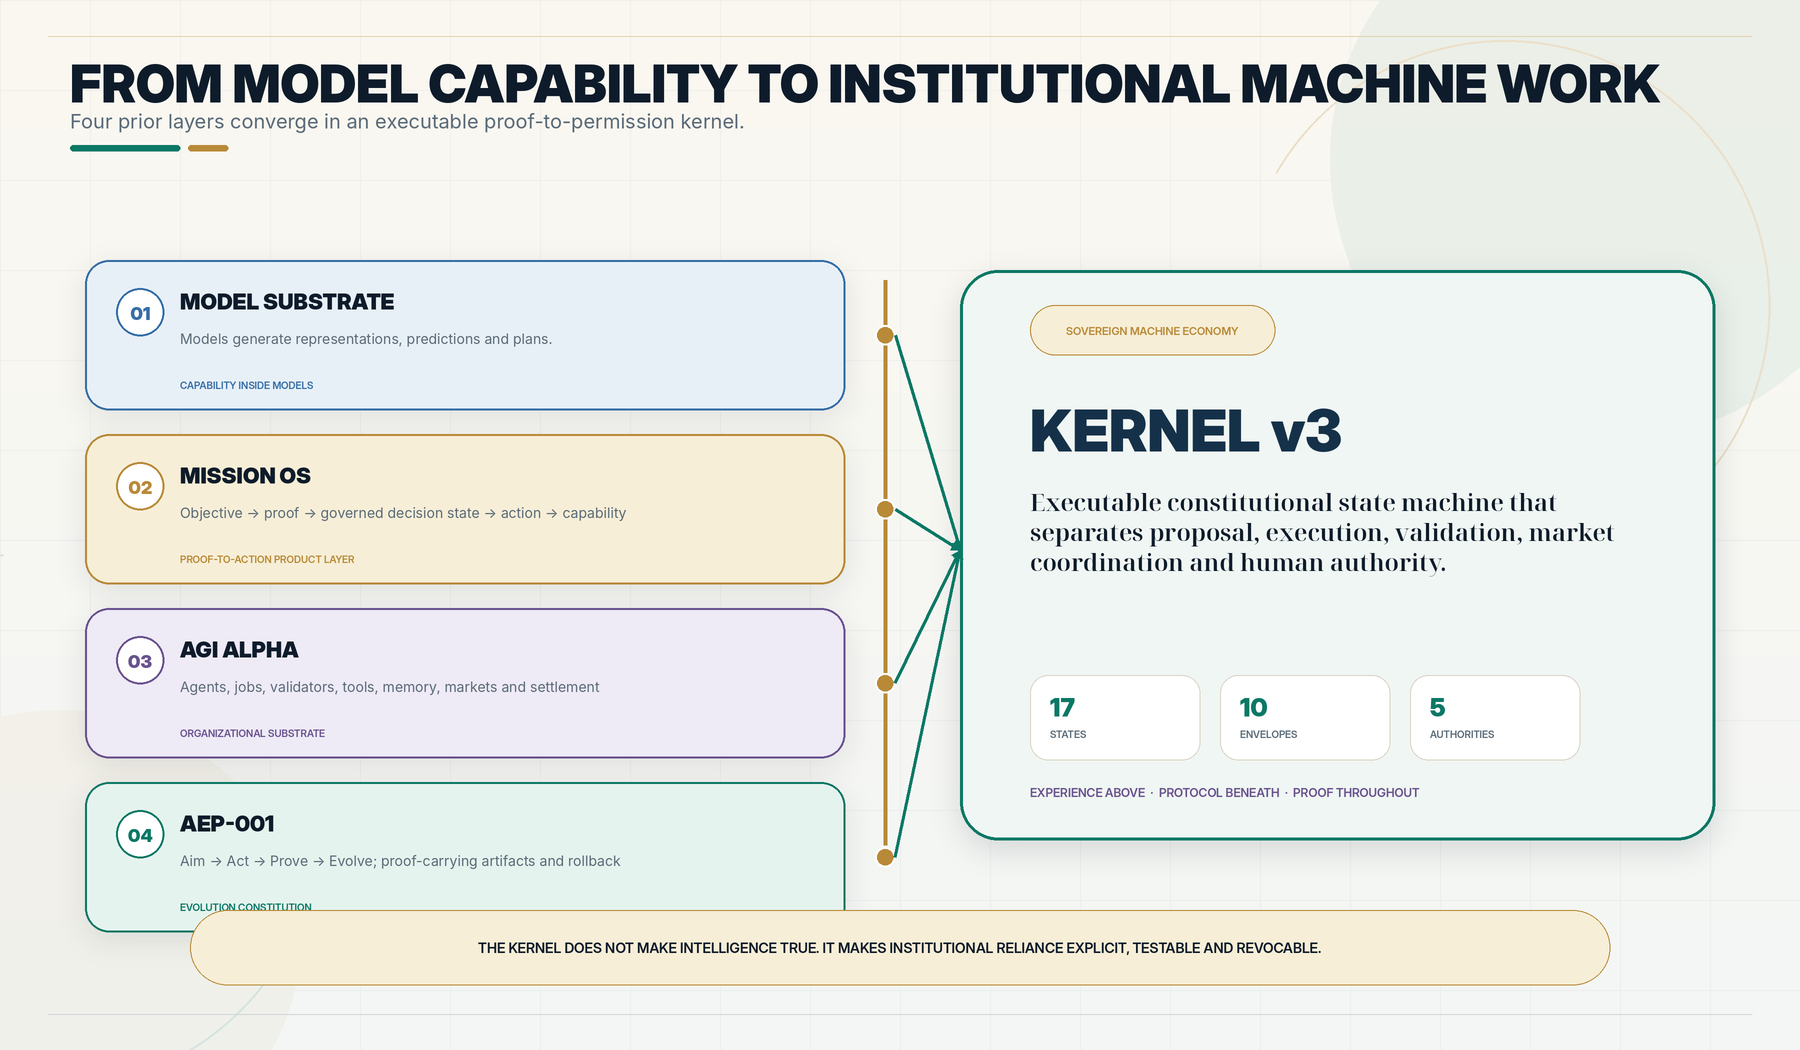
\includegraphics[width=6.75in,height=3.9375in]{media/image2.png}

Figure 1. The lineage from model capability, Mission OS, AGI ALPHA, and
AEP-001 to the executable Sovereign Machine Economy Kernel v3.

\subsection{1.1 The category: verifiable autonomous work
infrastructure}\label{the-category-verifiable-autonomous-work-infrastructure}

The proposed category is not another agent framework. It is verifiable
autonomous work infrastructure: the control plane that turns machine
activity into evidence-bearing, reviewable, policy-bound institutional
work. The product-level framing is the Proof OS for autonomous AI work.
The protocol-level framing is a constitutional kernel. The market-level
framing is a Sovereign Machine Economy. These are three views of the
same system.

"Sovereign" does not mean unconstrained machine autonomy. It means that
an institution retains control over its objectives, identities,
policies, evidence, memory, evaluators, and authorization boundary
rather than surrendering those functions to an opaque external agent.
"Machine economy" does not mean that live value moves in the reference
release. It means that work, proof, validation, dissent, reputation,
settlement intent, and reusable capability are represented as governed
economic objects.

\subsection{1.2 The proof-to-permission
distinction}\label{the-proof-to-permission-distinction}

Proof and permission are adjacent but different. A hash can show
integrity. A signature can show possession of a signing key. An external
attestation can report an independent assessment. A human certificate
can record a scoped institutional decision. None of these, alone,
establishes universal truth. None should silently invoke a consequential
action.

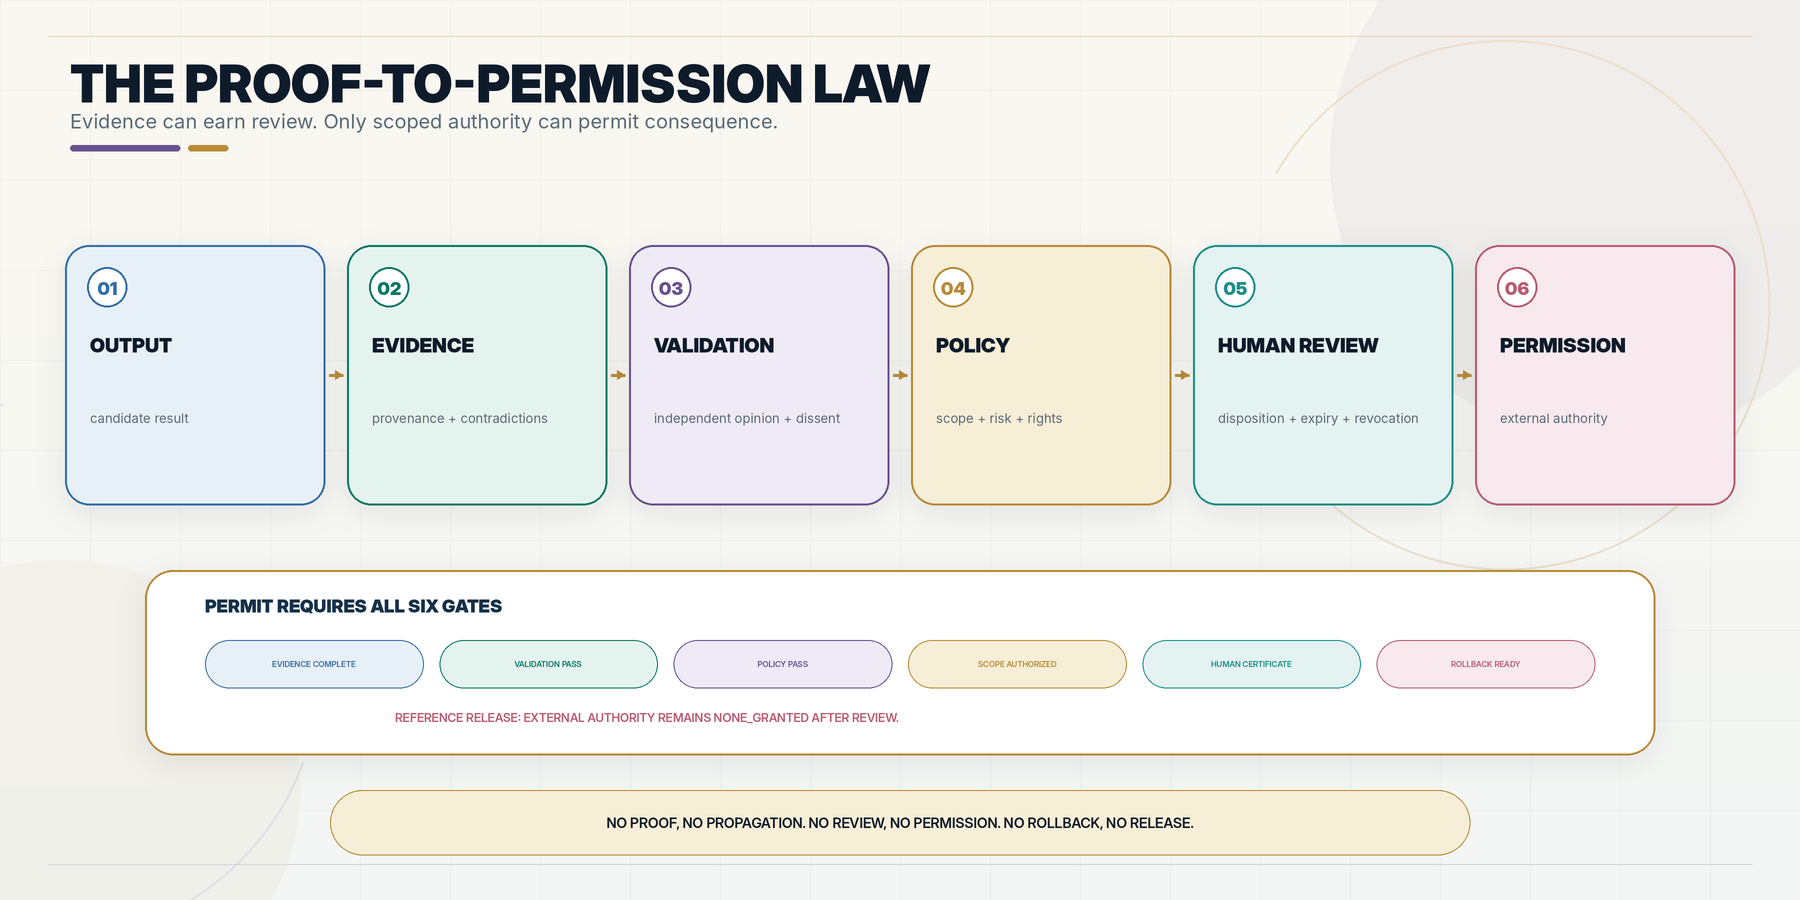
\includegraphics[width=6.75in,height=3.375in]{media/image3.png}

Figure 2. The proof-to-permission law. Evidence can earn review; only
scoped authority can permit consequence.

Kernel v3 therefore distinguishes three states that are often collapsed
in agent products: work completion, review completion, and external
authority. A mission can be technically complete while external
authority remains NONE\_\allowbreak{}GRANTED. This allows autonomous discovery and
bounded execution without falsely implying permission to deploy, settle,
publish a regulated claim, or promote durable memory.

\section{2. System lineage and unified
doctrine}\label{system-lineage-and-unified-doctrine}

\subsection{2.1 Mission OS: objective to governed decision
state}\label{mission-os-objective-to-governed-decision-state}

Mission OS defines the immediate user experience. A user supplies a
consequential objective, not merely a topic. The system converts it into
a mission contract, runs bounded research and analysis, assembles an
Evidence Docket, checks contradictions and risks, and emits a
human-review-ready Governed Decision State {[}1{]}. Its central product
law is: set the objective; GoalOS runs until proof is done.

\begin{longtable}[]{@{}
  >{\raggedright\arraybackslash}p{(\columnwidth - 0\tabcolsep) * \real{1.0000}}@{}}
\toprule\noalign{}
\begin{minipage}[b]{\linewidth}\raggedright
\textbf{MissionValue = (DecisionImpact × ProofIntegrity × Actionability
× Reuse) / (Cost + Risk + Latency + ProofDebt)}

(2)
\end{minipage} \\
\midrule\noalign{}
\endhead
\bottomrule\noalign{}
\endlastfoot
\end{longtable}

Proof debt is the institutional risk that unsupported AI output becomes
default policy, repeated fact, or reusable capability before it is
challenged. Kernel v3 operationalizes proof-debt reduction by making
claims, evidence, issuers, transitions, review, and memory disposition
explicit.

\subsection{2.2 AGI ALPHA: intelligence organizations above
models}\label{agi-alpha-intelligence-organizations-above-models}

AGI ALPHA argues that the Transformer scaled intelligence inside models,
while the next frontier is scaling intelligence across governed
organizations {[}2{]}. The organizational substrate includes agents,
jobs, validators, tools, memory, incentives, markets, settlement,
governance, and capacity allocation. The objective is not more agents
talking. It is proof-bearing machine labor: jobs are bounded, tool use
is traced, results are validated, capability is reusable, settlement is
auditable, and empirical claims require Evidence Dockets.

The Sovereign Machine Economy uses that substrate in a reduced,
executable form. META-AGENTIC α-AGI represents institution formation.
AGI Alpha Node represents bounded execution and receipts. AGI Jobs
represents markets, validation, dispute, and settlement intent. Kernel
v3 supplies the constitutional boundary that prevents those engines from
becoming a monolithic authority.

\subsection{2.3 AEP-001: proof-backed
evolution}\label{aep-001-proof-backed-evolution}

AEP-001 gives recursive improvement a constitution {[}3{]}. Its public
doctrine is Aim -\textgreater{} Act -\textgreater{} Prove
-\textgreater{} Evolve; its object lifecycle is Commit -\textgreater{}
Execute -\textgreater{} Prove -\textgreater{} Evolve. A proof-carrying
artifact earns the right to influence future work only after proof
integrity, evaluation, scope authorization, challenge, canary control,
monitoring, and rollback readiness. Kernel v3 inherits that doctrine but
keeps the reference implementation chain-agnostic and browser-local.

\subsection{2.4 Three nested doctrines}\label{three-nested-doctrines}

\begin{longtable}[]{@{}
  >{\raggedright\arraybackslash}p{(\columnwidth - 4\tabcolsep) * \real{0.3333}}
  >{\raggedright\arraybackslash}p{(\columnwidth - 4\tabcolsep) * \real{0.3333}}
  >{\raggedright\arraybackslash}p{(\columnwidth - 4\tabcolsep) * \real{0.3333}}@{}}
\toprule\noalign{}
\begin{minipage}[b]{\linewidth}\raggedright
\textbf{Level}
\end{minipage} & \begin{minipage}[b]{\linewidth}\raggedright
\textbf{Doctrine}
\end{minipage} & \begin{minipage}[b]{\linewidth}\raggedright
\textbf{Primary question}
\end{minipage} \\
\midrule\noalign{}
\endhead
\bottomrule\noalign{}
\endlastfoot
\textbf{Mission experience} & Identify -\textgreater{} Out-Learn
-\textgreater{} Out-Think -\textgreater{} Out-Design -\textgreater{}
Out-Strategise -\textgreater{} Out-Execute & How does the system move
from opportunity to bounded action? \\
\textbf{Constitutional lifecycle} & 17 typed, issuer-bound states & What
must be true before the next state may exist? \\
\textbf{Evolution law} & Aim -\textgreater{} Act -\textgreater{} Prove
-\textgreater{} Evolve & What earns the right to propagate into future
capability? \\
\end{longtable}

These doctrines are complementary. The six-phase chain is legible to
users. The state machine is enforceable by the runtime. The evolution
law governs reuse and propagation.

\section{3. The Sovereign Machine Economy
architecture}\label{the-sovereign-machine-economy-architecture}

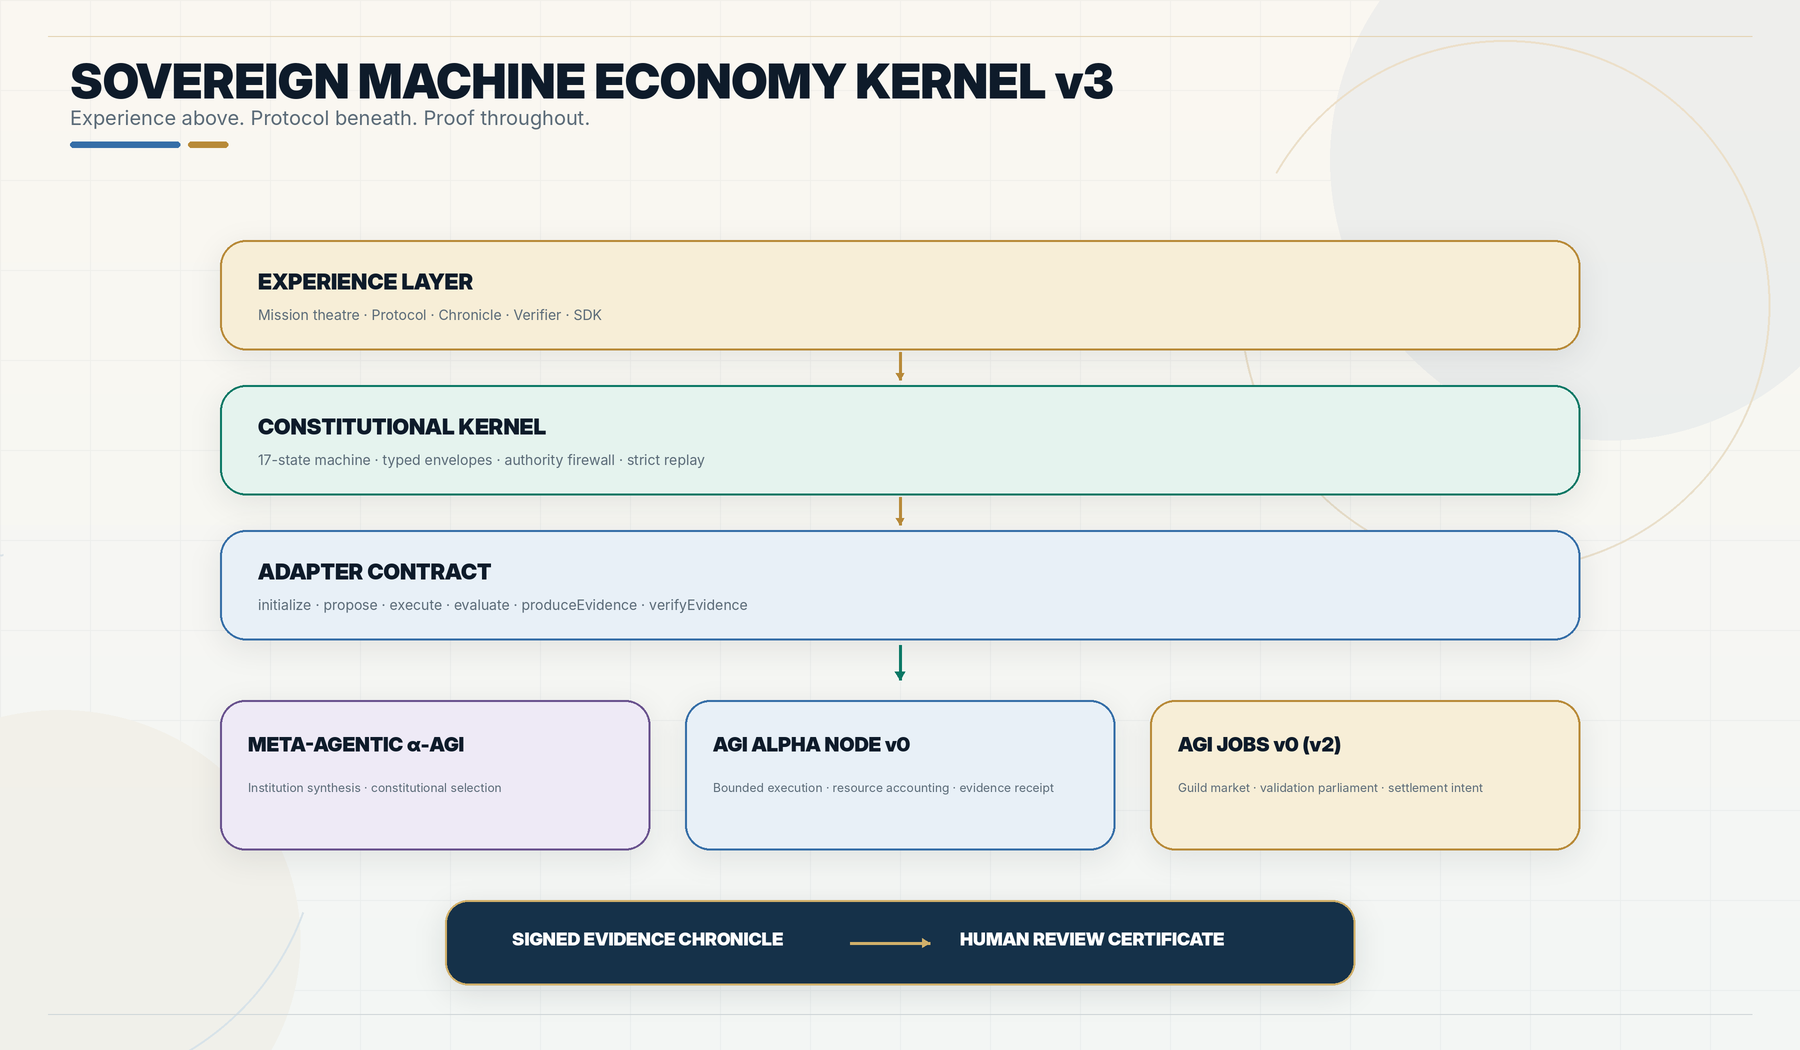
\includegraphics[width=6.75in,height=3.9375in]{media/image4.png}

Figure 3. Kernel v3 architecture: experience layer, constitutional
kernel, adapter contract, three engines, signed Chronicle, and Human
Review Certificate.

\subsection{3.1 META-AGENTIC α-AGI: institution
formation}\label{meta-agentic-ux3b1-agi-institution-formation}

The META-AGENTIC engine proposes bounded institutions rather than simply
choosing a prompt chain. It can synthesize alternative organizations,
assign roles, define information and tool boundaries, declare stop
conditions, and seal an institution charter. In the reference release it
is deterministic and local. It does not claim to discover an objectively
optimal institution, and it cannot execute or settle its own proposal.

\subsection{3.2 AGI Alpha Node v0: bounded
execution}\label{agi-alpha-node-v0-bounded-execution}

The Node engine admits an execution identity, resource envelope, primary
route, and shadow route. It emits execution receipts and seals evidence
commitments. The separation between primary and shadow routes supports
counterfactual challenge and failure detection. The Node may execute
bounded work and package evidence, but it cannot validate itself or
grant authority.

\subsection{3.3 AGI Jobs v0 (v2): proof-gated market
coordination}\label{agi-jobs-v0-v2-proof-gated-market-coordination}

The Jobs engine convenes agent guilds, records commitments and reveals,
forms an execution coalition, preserves validator opinions and dissent,
opens a challenge window, and prepares settlement intent. In the
reference release, settlement is demonstration-only and no live value
moves. The market steward may prepare a waterfall, but cannot authorize
transfer.

\subsection{3.4 Kernel v3: authority
firewall}\label{kernel-v3-authority-firewall}

Kernel v3 owns state advancement. Adapters may propose work, produce
receipts, or submit evidence. They do not mutate the state machine
directly. The kernel verifies the envelope, issuer, predecessor, payload
commitment, signature, state order, guard conditions, and authority
scope before an event is appended. This is the central design decision:
intelligence is replaceable; the constitution is not.

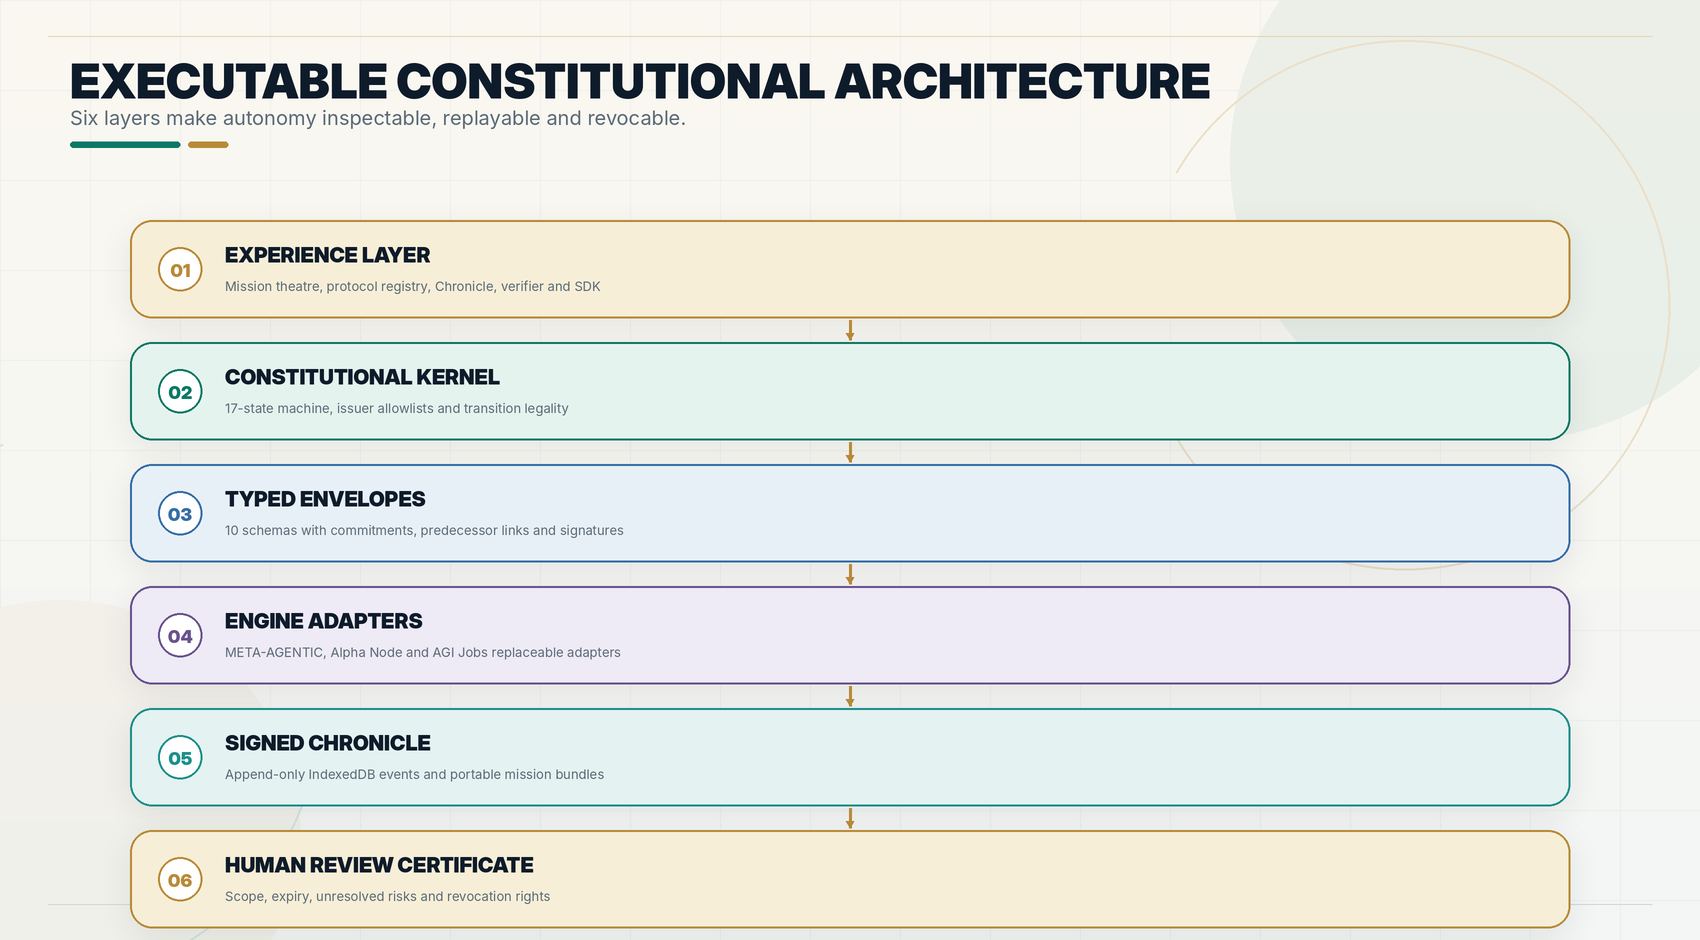
\includegraphics[width=6.75in,height=3.73235in]{media/image5.png}

Figure 4. The executable constitutional architecture. Experience sits
above the kernel; engines and signed evidence sit below the authority
boundary.

\section{4. Autonomous end-to-end operating
doctrine}\label{autonomous-end-to-end-operating-doctrine}

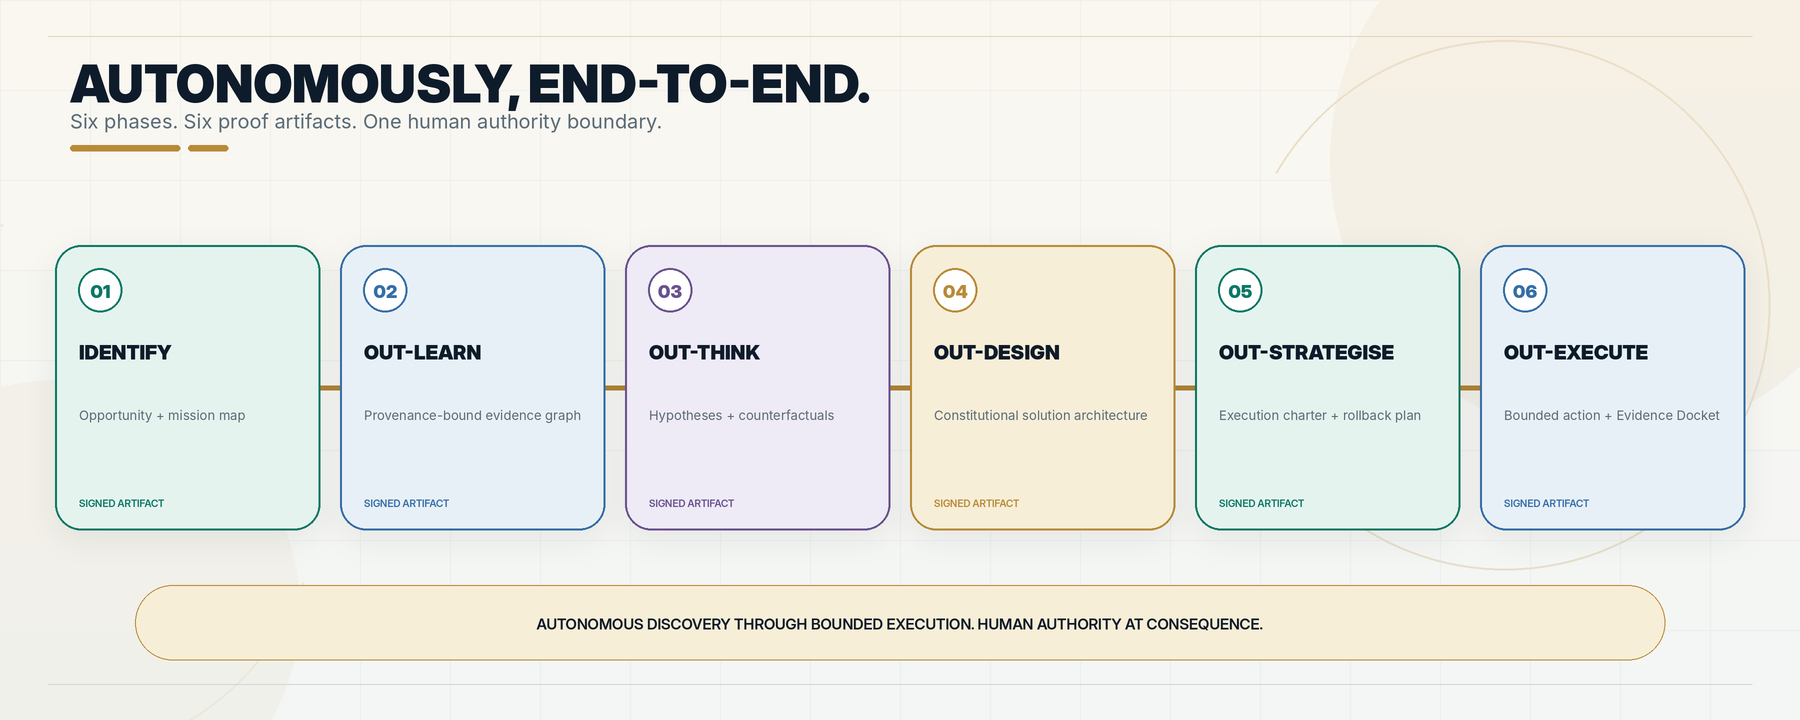
\includegraphics[width=6.75in,height=2.7in]{media/image6.png}

Figure 5. The six-phase autonomy chain. Each phase must produce a proof
artifact; human authority remains at consequential action.

The system is designed to operate autonomously from discovery through
bounded execution. It is not designed to grant itself consequential
authority. The six phases are therefore work-production phases, not
escalating permission levels.

\begin{longtable}[]{@{}
  >{\raggedright\arraybackslash}p{(\columnwidth - 6\tabcolsep) * \real{0.2500}}
  >{\raggedright\arraybackslash}p{(\columnwidth - 6\tabcolsep) * \real{0.2500}}
  >{\raggedright\arraybackslash}p{(\columnwidth - 6\tabcolsep) * \real{0.2500}}
  >{\raggedright\arraybackslash}p{(\columnwidth - 6\tabcolsep) * \real{0.2500}}@{}}
\toprule\noalign{}
\begin{minipage}[b]{\linewidth}\raggedright
\textbf{Phase}
\end{minipage} & \begin{minipage}[b]{\linewidth}\raggedright
\textbf{Core work}
\end{minipage} & \begin{minipage}[b]{\linewidth}\raggedright
\textbf{Required artifact}
\end{minipage} & \begin{minipage}[b]{\linewidth}\raggedright
\textbf{Failure condition}
\end{minipage} \\
\midrule\noalign{}
\endhead
\bottomrule\noalign{}
\endlastfoot
\textbf{Identify} & Detect opportunity, decision, stakeholder,
constraint, and risk surface. & Opportunity and mission map & No clear
decision, owner, success criterion, or stop condition. \\
\textbf{Out-Learn} & Gather and classify primary evidence, provenance,
freshness, and contradiction. & Provenance-bound evidence graph &
Sources are absent, stale, circular, or untraceable. \\
\textbf{Out-Think} & Generate hypotheses, alternatives, counterfactuals,
and unresolved questions. & Hypothesis and counterfactual dossier & A
single narrative survives only because alternatives were not tested. \\
\textbf{Out-Design} & Construct a solution architecture, institutional
roles, interfaces, and safety boundaries. & Constitutional solution
architecture & The design has no authority map, test plan, or failure
boundary. \\
\textbf{Out-Strategise} & Choose sequence, resources, validator plan,
challenge rights, monitoring, and rollback. & Execution charter and
rollback plan & The plan cannot stop, escalate, or revert safely. \\
\textbf{Out-Execute} & Run bounded work, seal evidence, validate, and
prepare review. & Execution receipt and Evidence Docket & The evidence
package is incomplete or authority is implied without review. \\
\end{longtable}

\subsection{4.1 Autonomy is not
authority}\label{autonomy-is-not-authority}

A system can autonomously identify, learn, reason, design, strategize,
and execute within a sandbox while remaining unauthorized to trigger
production consequences. This is not a contradiction. It is the intended
operating model. Autonomy concerns who performs the work; authority
concerns who may create institutional consequence.

\begin{longtable}[]{@{}
  >{\raggedright\arraybackslash}p{(\columnwidth - 0\tabcolsep) * \real{1.0000}}@{}}
\toprule\noalign{}
\begin{minipage}[b]{\linewidth}\raggedright
\textbf{Constitutional invariant.}

Autonomous discovery through bounded execution. Human authority at
consequence. Human review records scope; it does not trigger execution.
\end{minipage} \\
\midrule\noalign{}
\endhead
\bottomrule\noalign{}
\endlastfoot
\end{longtable}

\section{5. Formal kernel model}\label{formal-kernel-model}

Define the kernel as a labeled transition system K = (S, E, R, δ, G, C),
where S is the set of constitutional states, E is the set of typed
envelopes, R is the set of issuer roles, δ is the transition function, G
is the set of guards, and C is the append-only commitment Chronicle.

\begin{longtable}[]{@{}
  >{\raggedright\arraybackslash}p{(\columnwidth - 0\tabcolsep) * \real{1.0000}}@{}}
\toprule\noalign{}
\begin{minipage}[b]{\linewidth}\raggedright
\textbf{δ(s\_\allowbreak{}t, e\_\allowbreak{}t) = s\_\allowbreak{}(t+1) iff Schema(e\_\allowbreak{}t) \(\wedge\) IssuerAllowed(e\_\allowbreak{}t)
\(\wedge\) Prev(e\_\allowbreak{}t)=head(C\_\allowbreak{}t) \(\wedge\) PayloadHashValid(e\_\allowbreak{}t) \(\wedge\) SignatureValid(e\_\allowbreak{}t)
\(\wedge\) GuardPass(s\_\allowbreak{}t,e\_\allowbreak{}t)}

(3)
\end{minipage} \\
\midrule\noalign{}
\endhead
\bottomrule\noalign{}
\endlastfoot
\end{longtable}

The transition function is partial: malformed, unauthorized,
out-of-order, unsigned, tampered, or guard-failing envelopes have no
valid successor. A rejected proposal does not partially advance the
mission. It is quarantined or fails closed.

\subsection{5.1 Mission object}\label{mission-object}

\begin{longtable}[]{@{}
  >{\raggedright\arraybackslash}p{(\columnwidth - 0\tabcolsep) * \real{1.0000}}@{}}
\toprule\noalign{}
\begin{minipage}[b]{\linewidth}\raggedright
Mission = \{\\
objective, decisionToSupport, successCriteria, failureCriteria,\\
constraints, riskClass, posture, allowedTools, prohibitedActions,\\
requiredEvidence, validators, reviewRequirement, rollbackObligations\\
\}\strut
\end{minipage} \\
\midrule\noalign{}
\endhead
\bottomrule\noalign{}
\endlastfoot
\end{longtable}

\subsection{5.2 Envelope object}\label{envelope-object}

\begin{longtable}[]{@{}
  >{\raggedright\arraybackslash}p{(\columnwidth - 0\tabcolsep) * \real{1.0000}}@{}}
\toprule\noalign{}
\begin{minipage}[b]{\linewidth}\raggedright
Envelope = \{\\
protocolVersion, schemaId, envelopeType, issuerRole, issuerKeyId,\\
sourceState, targetState, predecessorCommitment, logicalClock,\\
authorityScope, payload, payloadCommitment, envelopeId, signature\\
\}\strut
\end{minipage} \\
\midrule\noalign{}
\endhead
\bottomrule\noalign{}
\endlastfoot
\end{longtable}

\subsection{5.3 Acceptance law}\label{acceptance-law}

The kernel does not ask whether an envelope is persuasive. It asks
whether the envelope is structurally valid, issued by the permitted
role, correctly linked, correctly signed, compatible with the current
state, and sufficient for the target guard. This transforms state
advancement from conversational convention into an auditable protocol
decision.

\begin{longtable}[]{@{}
  >{\raggedright\arraybackslash}p{(\columnwidth - 0\tabcolsep) * \real{1.0000}}@{}}
\toprule\noalign{}
\begin{minipage}[b]{\linewidth}\raggedright
\textbf{Accept(e\_\allowbreak{}t) \(\in\) \{ACCEPT, QUARANTINE, SAFE\_\allowbreak{}HOLD\}; there is no
partial trust state.}

(4)
\end{minipage} \\
\midrule\noalign{}
\endhead
\bottomrule\noalign{}
\endlastfoot
\end{longtable}

\section{6. Seventeen constitutional
states}\label{seventeen-constitutional-states}

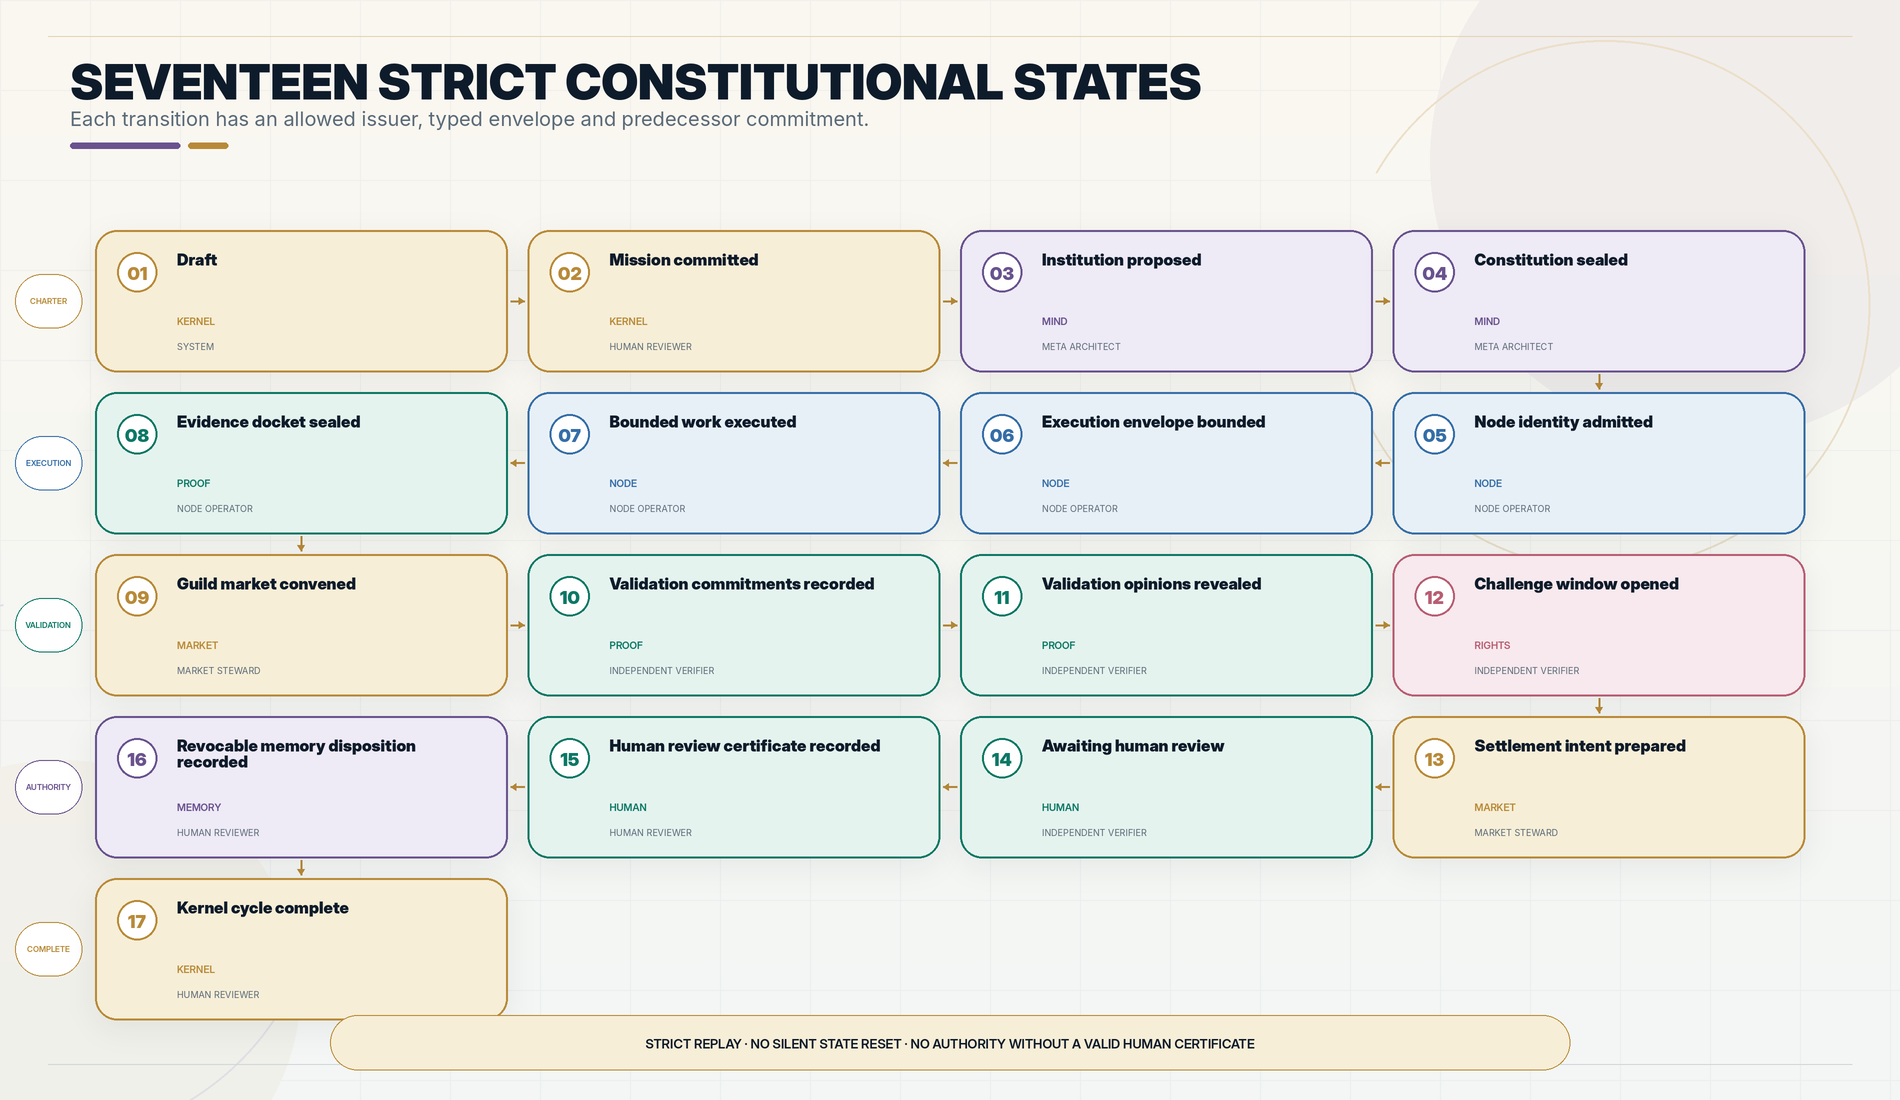
\includegraphics[width=6.75in,height=3.90789in]{media/image7.png}

Figure 6. The 17-state constitutional lifecycle, from Draft to Kernel
Cycle Complete.

The lifecycle deliberately separates work planes and issuer roles.
Mission commitment is human-initiated. Institution formation belongs to
the Meta-Architect. Node admission and bounded work belong to the Node
Operator. Validation and challenge belong to the Independent Verifier.
Settlement intent belongs to the Market Steward. Review and memory
disposition belong to the Human Reviewer.

\begin{longtable}[]{@{}
  >{\raggedright\arraybackslash}p{(\columnwidth - 6\tabcolsep) * \real{0.2500}}
  >{\raggedright\arraybackslash}p{(\columnwidth - 6\tabcolsep) * \real{0.2500}}
  >{\raggedright\arraybackslash}p{(\columnwidth - 6\tabcolsep) * \real{0.2500}}
  >{\raggedright\arraybackslash}p{(\columnwidth - 6\tabcolsep) * \real{0.2500}}@{}}
\toprule\noalign{}
\begin{minipage}[b]{\linewidth}\raggedright
\textbf{\#}
\end{minipage} & \begin{minipage}[b]{\linewidth}\raggedright
\textbf{State}
\end{minipage} & \begin{minipage}[b]{\linewidth}\raggedright
\textbf{Plane}
\end{minipage} & \begin{minipage}[b]{\linewidth}\raggedright
\textbf{Permitted issuer}
\end{minipage} \\
\midrule\noalign{}
\endhead
\bottomrule\noalign{}
\endlastfoot
\textbf{1} & Draft & KERNEL & System \\
\textbf{2} & Mission Committed & KERNEL & Human Reviewer \\
\textbf{3} & Institution Proposed & MIND & Meta Architect \\
\textbf{4} & Institution Chartered & MIND & Meta Architect \\
\textbf{5} & Node Admitted & NODE & Node Operator \\
\textbf{6} & Execution Bounded & NODE & Node Operator \\
\textbf{7} & Work Executed & NODE & Node Operator \\
\textbf{8} & Evidence Sealed & PROOF & Node Operator \\
\textbf{9} & Market Convened & MARKET & Market Steward \\
\textbf{10} & Validation Committed & PROOF & Independent Verifier \\
\textbf{11} & Validation Revealed & PROOF & Independent Verifier \\
\textbf{12} & Challenge Window Open & RIGHTS & Independent Verifier \\
\textbf{13} & Settlement Intent Prepared & MARKET & Market Steward \\
\textbf{14} & Awaiting Human Review & HUMAN & Independent Verifier \\
\textbf{15} & Human Review Recorded & HUMAN & Human Reviewer \\
\textbf{16} & Memory Disposition Recorded & MEMORY & Human Reviewer \\
\textbf{17} & Complete & KERNEL & Human Reviewer \\
\end{longtable}

\subsection{6.1 Terminal and fail-closed
states}\label{terminal-and-fail-closed-states}

The normal machine-complete state is AWAITING\_\allowbreak{}HUMAN\_\allowbreak{}REVIEW. The full
local cycle may reach COMPLETE only after a Human Review Certificate and
memory disposition are recorded. Adversarial or deficient scenarios
terminate differently: identity drift enters SAFE\_\allowbreak{}HOLD; evidence gaps
may open DISPUTE\_\allowbreak{}OPEN; budget or policy breaches can require
HUMAN\_\allowbreak{}REVIEW\_\allowbreak{}REQUIRED. These terminal states are explicit outputs, not
exceptions hidden in logs.

\subsection{6.2 Completion does not imply
permission}\label{completion-does-not-imply-permission}

COMPLETE means that the local constitutional record is internally
complete. It does not mean that a live transaction, deployment,
publication, medical intervention, legal filing, market action, or
production change is authorized. External action requires a separate,
environment-specific activation layer that is intentionally absent from
the reference release.

\section{7. Ten typed protocol
envelopes}\label{ten-typed-protocol-envelopes}

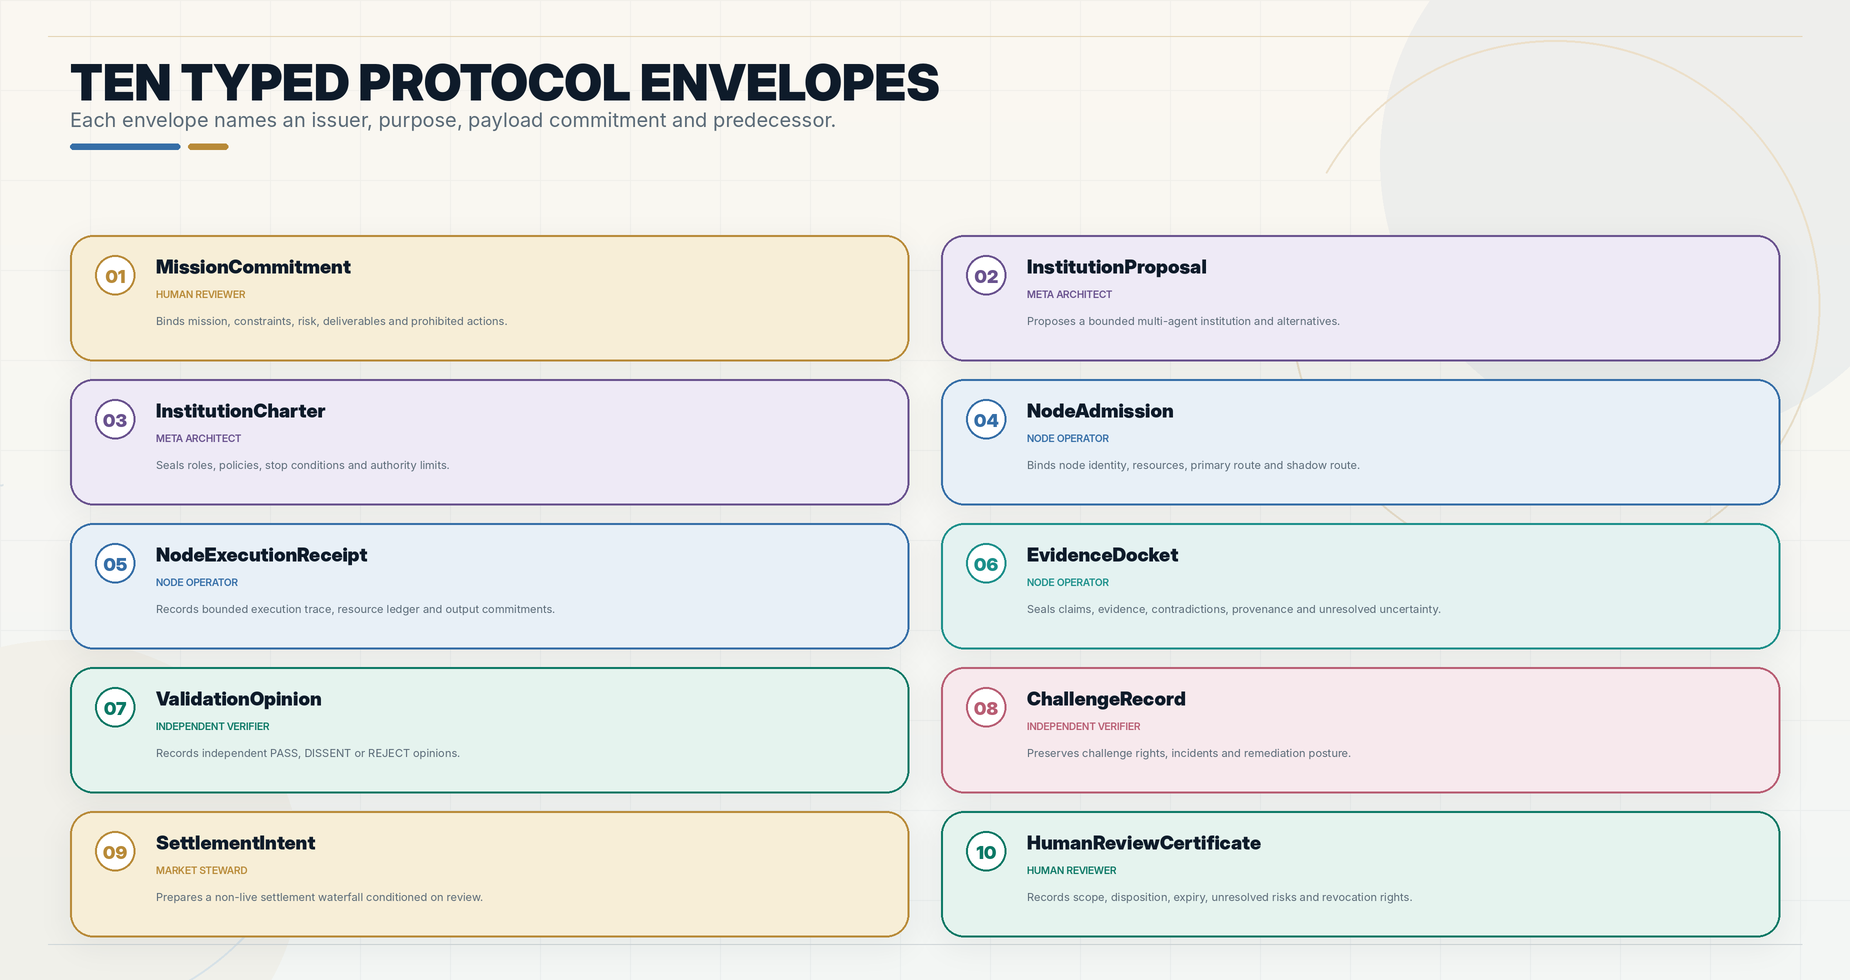
\includegraphics[width=6.75in,height=3.57568in]{media/image8.png}

Figure 7. The ten envelope types that carry mission, institution, node,
evidence, validation, challenge, settlement, and review records.

\begin{longtable}[]{@{}
  >{\raggedright\arraybackslash}p{(\columnwidth - 4\tabcolsep) * \real{0.3333}}
  >{\raggedright\arraybackslash}p{(\columnwidth - 4\tabcolsep) * \real{0.3333}}
  >{\raggedright\arraybackslash}p{(\columnwidth - 4\tabcolsep) * \real{0.3333}}@{}}
\toprule\noalign{}
\begin{minipage}[b]{\linewidth}\raggedright
\textbf{Envelope}
\end{minipage} & \begin{minipage}[b]{\linewidth}\raggedright
\textbf{Issuer}
\end{minipage} & \begin{minipage}[b]{\linewidth}\raggedright
\textbf{Purpose}
\end{minipage} \\
\midrule\noalign{}
\endhead
\bottomrule\noalign{}
\endlastfoot
\textbf{MissionCommitment} & Human Reviewer & Binds mission,
constraints, risk, deliverables, prohibited actions, and review
requirement. \\
\textbf{InstitutionProposal} & Meta-Architect & Proposes a bounded
institution and alternatives. \\
\textbf{InstitutionCharter} & Meta-Architect & Seals roles, policies,
stop conditions, and authority limits. \\
\textbf{NodeAdmission} & Node Operator & Binds node identity, resources,
primary route, and shadow route. \\
\textbf{NodeExecutionReceipt} & Node Operator & Records bounded
execution trace, resources, outputs, and commitments. \\
\textbf{EvidenceDocket} & Node Operator & Seals claims, evidence,
contradictions, provenance, and unresolved uncertainty. \\
\textbf{ValidationOpinion} & Independent Verifier & Records PASS,
DISSENT, or REJECT opinions and evidence references. \\
\textbf{ChallengeRecord} & Independent Verifier & Preserves challenge
rights, incidents, remediation, and dispute posture. \\
\textbf{SettlementIntent} & Market Steward & Prepares a non-live
allocation or settlement waterfall conditioned on review. \\
\textbf{HumanReviewCertificate} & Human Reviewer & Records disposition,
scope, expiry, unresolved risks, memory posture, and revocation. \\
\end{longtable}

\subsection{7.1 Canonicalization}\label{canonicalization}

Commitments are only reproducible if equivalent payloads serialize
consistently. The reference implementation uses deterministic canonical
JSON. Production profiles should formally specify canonicalization and
may align with the JSON Canonicalization Scheme in RFC 8785 {[}6{]}. The
paper does not claim full RFC 8785 conformance for the current
implementation.

\subsection{7.2 Logical time}\label{logical-time}

The kernel uses a logical clock inside the signed event history. Logical
time avoids reliance on wall-clock timestamps as the sole ordering
authority. Production profiles may add trusted time attestations, but
state order remains grounded in predecessor commitments and legal
transitions.

\section{8. Role separation and cryptographic
authority}\label{role-separation-and-cryptographic-authority}

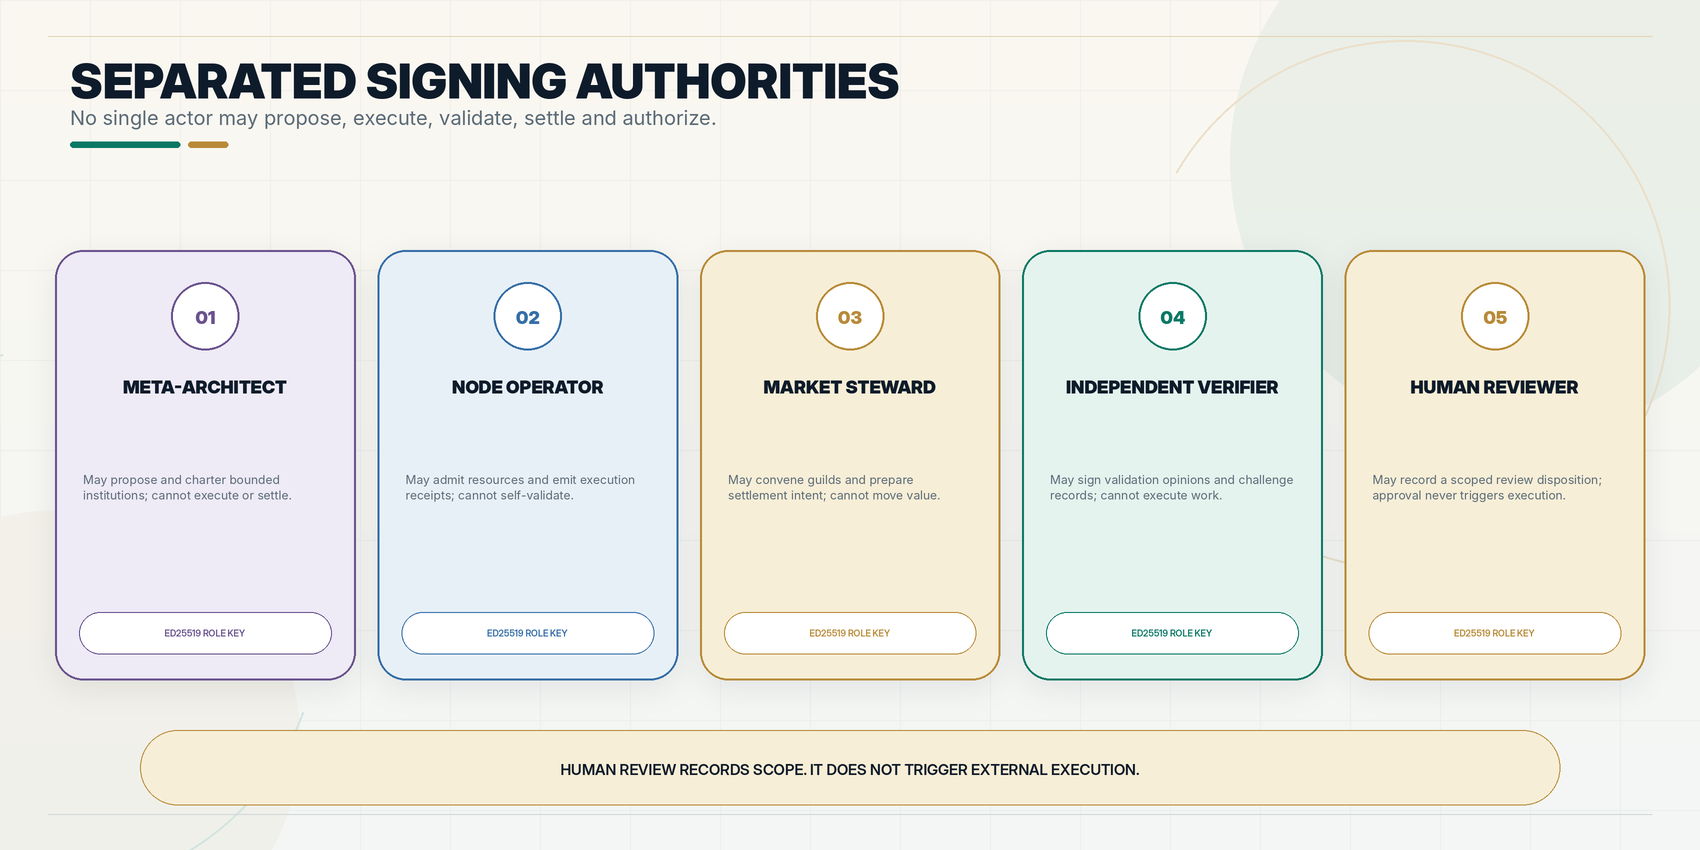
\includegraphics[width=6.75in,height=3.375in]{media/image9.png}

Figure 8. Five separated signing authorities. No single role may
propose, execute, validate, settle, and authorize.

Separation of duties is a constitutional property, not a user-interface
convention. NIST AI RMF identifies role separation between builders and
those performing verification and validation as a best practice across
the AI lifecycle {[}11{]}. Kernel v3 extends this principle into the
event protocol: each transition names an issuer role, and the worker
checks the issuer allowlist before append.

\begin{longtable}[]{@{}
  >{\raggedright\arraybackslash}p{(\columnwidth - 4\tabcolsep) * \real{0.3333}}
  >{\raggedright\arraybackslash}p{(\columnwidth - 4\tabcolsep) * \real{0.3333}}
  >{\raggedright\arraybackslash}p{(\columnwidth - 4\tabcolsep) * \real{0.3333}}@{}}
\toprule\noalign{}
\begin{minipage}[b]{\linewidth}\raggedright
\textbf{Role}
\end{minipage} & \begin{minipage}[b]{\linewidth}\raggedright
\textbf{May}
\end{minipage} & \begin{minipage}[b]{\linewidth}\raggedright
\textbf{Must not}
\end{minipage} \\
\midrule\noalign{}
\endhead
\bottomrule\noalign{}
\endlastfoot
\textbf{Meta-Architect} & Propose and charter bounded institutions. &
Execute work, validate its own institution, prepare settlement, or
authorize consequence. \\
\textbf{Node Operator} & Admit resources, execute bounded work, emit
receipts, and seal the initial Evidence Docket. & Self-validate,
authorize settlement, or issue human review. \\
\textbf{Market Steward} & Convene guilds and prepare non-live settlement
intent. & Move value, rewrite evidence, or validate execution. \\
\textbf{Independent Verifier} & Commit and reveal validation opinions,
preserve dissent, open challenge records. & Execute the work or control
market allocation. \\
\textbf{Human Reviewer} & Record scoped disposition, conditions, expiry,
revocation, and memory posture. & Silently invoke external execution or
convert local signature into legal identity. \\
\end{longtable}

\subsection{8.1 Ed25519 keys}\label{ed25519-keys}

The browser-local reference generates distinct Ed25519 key pairs through
WebCrypto. RFC 8032 defines Ed25519 and its signing and verification
procedures {[}5{]}; Web Cryptography Level 2 exposes Ed25519 operations
through browser CryptoKey interfaces {[}7{]}. Portable bundles export
only public key material and fingerprints. Private keys remain local and
non-exported where supported.

\subsection{8.2 What a signature proves}\label{what-a-signature-proves}

A valid signature proves that the holder of a corresponding private key
approved the signed bytes. It does not prove the legal identity,
competence, independence, institutional mandate, or truthfulness of the
signer. Production systems therefore need identity binding, credential
governance, key custody, revocation, and possibly verifiable credentials
or external attestations {[}10{]}.

\subsection{8.3 Key compromise and
rotation}\label{key-compromise-and-rotation}

The reference release does not claim enterprise key management. A
production profile must define hardware or managed key custody,
rotation, revocation, threshold signatures where appropriate, incident
response, and the treatment of events signed by a later-compromised key.
The Chronicle must preserve history rather than rewrite it; remediation
occurs through new revocation and supersession events.

\section{9. Worker-owned execution and append-only
Chronicle}\label{worker-owned-execution-and-append-only-chronicle}

The browser interface is not the authority. The user interface proposes
envelopes to a dedicated Web Worker. Workers communicate through
structured messages and execute in a separate worker global scope
{[}9{]}. The worker reconstructs canonical payloads, verifies transition
legality, issuer authority, predecessor commitment, payload hash, and
signature, and returns an accepted event only when all checks pass.

\subsection{9.1 Commitment chain}\label{commitment-chain}

\begin{longtable}[]{@{}
  >{\raggedright\arraybackslash}p{(\columnwidth - 0\tabcolsep) * \real{1.0000}}@{}}
\toprule\noalign{}
\begin{minipage}[b]{\linewidth}\raggedright
\textbf{c\_\allowbreak{}0 = 0\^{}256; c\_\allowbreak{}t = H(c\_\allowbreak{}(t-1) \textbar\textbar{}\allowbreak{}
H(payload\_\allowbreak{}t) \textbar\textbar{}\allowbreak{} metadata\_\allowbreak{}t)}

(5)
\end{minipage} \\
\midrule\noalign{}
\endhead
\bottomrule\noalign{}
\endlastfoot
\end{longtable}

Each event contains the previous event commitment. Modifying a prior
payload changes its payload hash, its event commitment, every descendant
predecessor link, and the mission root. This is tamper evidence, not
immutable truth: the kernel can show that a record changed; it cannot
prove that the original observation was factually correct.

\subsection{9.2 IndexedDB Chronicle}\label{indexeddb-chronicle}

Accepted events are persisted in a local IndexedDB Chronicle. IndexedDB
provides object stores, versioned databases, transactions, and access
from pages or workers {[}8{]}. Kernel v3 uses it as an append-only
application discipline: accepted history is never edited in place.
Rollback, revocation, and correction are represented as new events that
reference prior state.

\subsection{9.3 Portable mission
bundles}\label{portable-mission-bundles}

A portable bundle contains protocol identifiers, mission metadata,
public role keys, event history, commitments, review records, memory
disposition, and derived roots. Export enables external inspection;
import is read-only until verification succeeds. A malformed or tampered
bundle is quarantined rather than partially loaded.

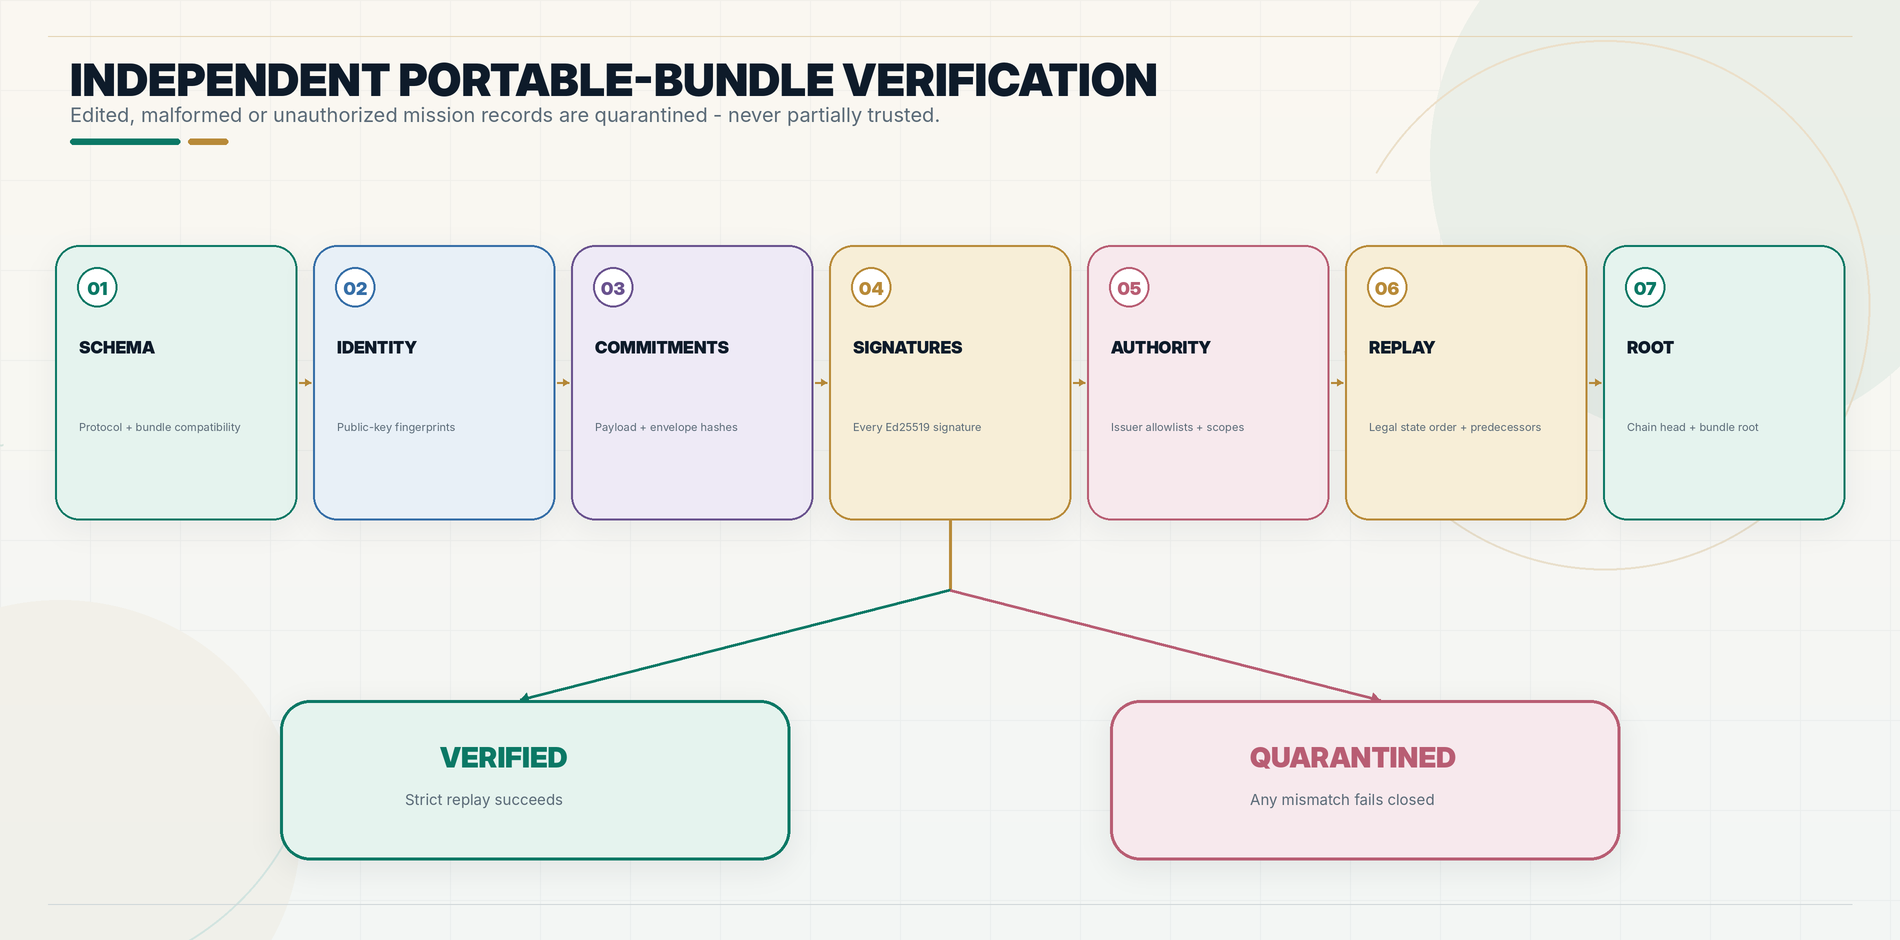
\includegraphics[width=6.75in,height=3.33947in]{media/image10.png}

Figure 9. Independent portable-bundle verification. Any mismatch in
schema, identity, commitment, signature, authority, replay, or root
fails closed.

\subsection{9.4 Evidence-status
separation}\label{evidence-status-separation}

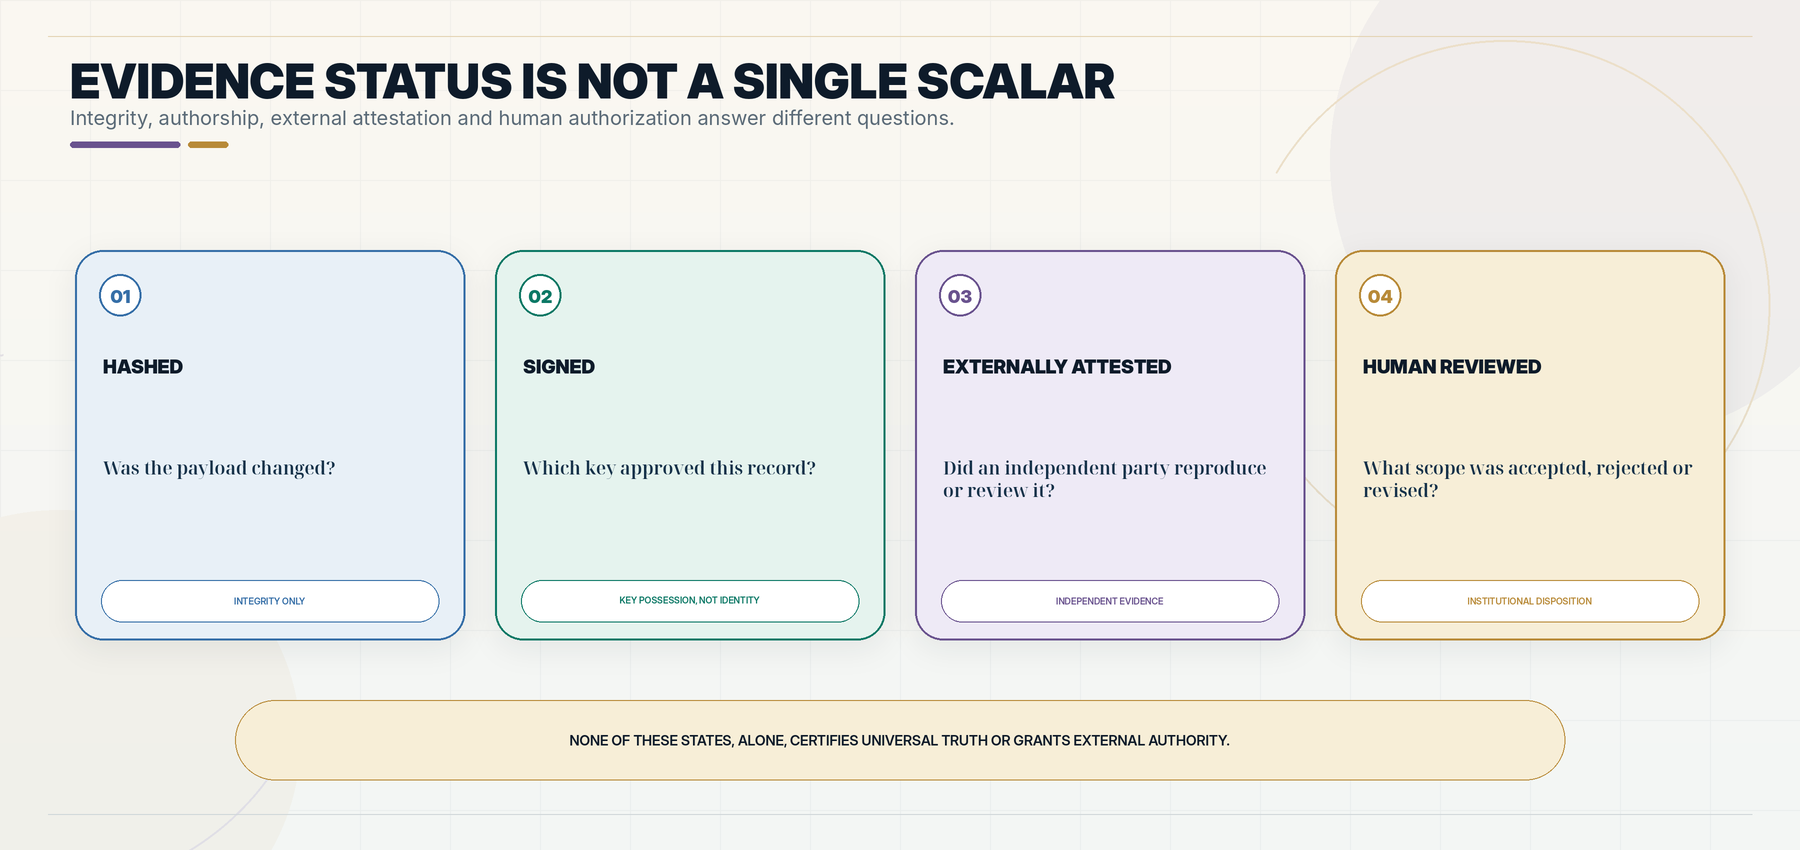
\includegraphics[width=6.75in,height=3.1875in]{media/image11.png}

Figure 10. Evidence status is multidimensional. Integrity, authorship,
attestation, and human review are not interchangeable.

\section{10. Replaceable adapter
contract}\label{replaceable-adapter-contract}

The kernel does not hard-code one model, agent framework, evaluator, or
chain. Each engine implements the same minimal adapter interface:
initialize, propose, execute, evaluate, produceEvidence, and
verifyEvidence. The contract is intentionally small so intelligence can
evolve without rewriting the state machine.

\begin{longtable}[]{@{}
  >{\raggedright\arraybackslash}p{(\columnwidth - 0\tabcolsep) * \real{1.0000}}@{}}
\toprule\noalign{}
\begin{minipage}[b]{\linewidth}\raggedright
interface AdapterContract \{\\
initialize(context)\\
propose(input)\\
execute(input)\\
evaluate(input)\\
produceEvidence(input)\\
verifyEvidence(input)\\
\}\strut
\end{minipage} \\
\midrule\noalign{}
\endhead
\bottomrule\noalign{}
\endlastfoot
\end{longtable}

\begin{longtable}[]{@{}
  >{\raggedright\arraybackslash}p{(\columnwidth - 4\tabcolsep) * \real{0.3333}}
  >{\raggedright\arraybackslash}p{(\columnwidth - 4\tabcolsep) * \real{0.3333}}
  >{\raggedright\arraybackslash}p{(\columnwidth - 4\tabcolsep) * \real{0.3333}}@{}}
\toprule\noalign{}
\begin{minipage}[b]{\linewidth}\raggedright
\textbf{Method}
\end{minipage} & \begin{minipage}[b]{\linewidth}\raggedright
\textbf{Responsibility}
\end{minipage} & \begin{minipage}[b]{\linewidth}\raggedright
\textbf{Forbidden shortcut}
\end{minipage} \\
\midrule\noalign{}
\endhead
\bottomrule\noalign{}
\endlastfoot
\textbf{initialize} & Bind scope, policy, capability declarations, and
permitted resources. & May not expand its own authority. \\
\textbf{propose} & Return a bounded plan, institution, route, or market
proposal. & May not commit the proposal directly. \\
\textbf{execute} & Perform permitted work and return a receipt. & May
not mark its own work valid. \\
\textbf{evaluate} & Score outputs or claims under an assigned rubric. &
May not collapse execution and independent validation. \\
\textbf{produceEvidence} & Package artifacts, provenance,
contradictions, cost, risk, and trace commitments. & May not label
generated evidence externally attested. \\
\textbf{verifyEvidence} & Check schema, provenance, signatures, tests,
and declared conditions. & May not grant external authority or promote
memory. \\
\end{longtable}

\subsection{10.1 Reference adapters}\label{reference-adapters}

The current META-AGENTIC, Alpha Node, and AGI Jobs adapters are
deterministic local fixtures. They demonstrate contract shape, state
advancement, proof packaging, failure injection, and replay. They are
not live model integrations, independent evaluators, production nodes,
or settlement services. This boundary is deliberate: the constitutional
kernel is tested before external capability is attached.

\subsection{10.2 Production adapter
admission}\label{production-adapter-admission}

A production adapter should declare identity, model or service version,
allowed data classes, tool scopes, network policy, evidence sources,
failure modes, cost model, evaluator independence, and revocation path.
Admission should require conformance tests, adversarial cases,
deterministic or bounded replay where possible, and a clear rule for
what remains unverifiable.

\begin{longtable}[]{@{}
  >{\raggedright\arraybackslash}p{(\columnwidth - 0\tabcolsep) * \real{1.0000}}@{}}
\toprule\noalign{}
\begin{minipage}[b]{\linewidth}\raggedright
\textbf{Adapter law.}

Replace the intelligence, never the constitution. An adapter may change
how work is proposed, executed, or evaluated. It may not change who is
permitted to advance a state.
\end{minipage} \\
\midrule\noalign{}
\endhead
\bottomrule\noalign{}
\endlastfoot
\end{longtable}

\section{11. Evidence Docket and Governed Decision
State}\label{evidence-docket-and-governed-decision-state}

The Evidence Docket is the institutional proof room. It connects the
mission contract to claims, sources, contradictions, execution receipts,
validator opinions, challenge records, cost and risk ledgers, review
disposition, and replay path. It is not a marketing page and not a
certificate of truth {[}1,3{]}.

\begin{longtable}[]{@{}
  >{\raggedright\arraybackslash}p{(\columnwidth - 4\tabcolsep) * \real{0.3333}}
  >{\raggedright\arraybackslash}p{(\columnwidth - 4\tabcolsep) * \real{0.3333}}
  >{\raggedright\arraybackslash}p{(\columnwidth - 4\tabcolsep) * \real{0.3333}}@{}}
\toprule\noalign{}
\begin{minipage}[b]{\linewidth}\raggedright
\textbf{Docket element}
\end{minipage} & \begin{minipage}[b]{\linewidth}\raggedright
\textbf{Minimum content}
\end{minipage} & \begin{minipage}[b]{\linewidth}\raggedright
\textbf{Institutional question}
\end{minipage} \\
\midrule\noalign{}
\endhead
\bottomrule\noalign{}
\endlastfoot
\textbf{Manifest} & Mission ID, release, signer set, protocol version,
public/private boundary. & What is this package and who is accountable
for it? \\
\textbf{Mission contract} & Objective, decision, constraints,
success/failure, risk, prohibited actions. & What was actually
commissioned? \\
\textbf{Claims matrix} & Claim, status, supporting evidence,
uncertainty, contradiction, owner. & Which claims are supported,
disputed, or unresolved? \\
\textbf{Source provenance} & Primary/secondary classification,
freshness, hash or pointer, license boundary. & Where did the evidence
come from? \\
\textbf{Execution receipts} & Routes, tools, resources, output
commitments, failures, blocked actions. & What did the machine do? \\
\textbf{Validation record} & Commitments, reveals, PASS/DISSENT/REJECT,
rationale, challenge window. & Who evaluated the work and how
independent were they? \\
\textbf{Risk and cost ledgers} & Known risk, residual risk, cost,
latency, governance overhead. & What did the work cost and what remains
dangerous? \\
\textbf{Human Review Certificate} & Disposition, scope, conditions,
expiry, revocation, settlement and memory posture. & What may the
institution rely on, and under which limits? \\
\textbf{Replay and rollback} & Bundle root, verification steps, rollback
target, remediation path. & Can the claim be challenged, replayed, or
reversed? \\
\end{longtable}

\subsection{11.1 Governed Decision State}\label{governed-decision-state}

The flagship deliverable is not a report. It is a Governed Decision
State: an inspectable, challengeable, operational package that makes
options, evidence, risk, uncertainty, authority, and next actions
legible. A report can be convincing while remaining non-operational. A
governed state can be accepted, rejected, revised, disputed, scoped,
expired, revoked, replayed, and converted into a bounded action graph.

\subsection{11.2 Proof debt}\label{proof-debt}

\begin{longtable}[]{@{}
  >{\raggedright\arraybackslash}p{(\columnwidth - 0\tabcolsep) * \real{1.0000}}@{}}
\toprule\noalign{}
\begin{minipage}[b]{\linewidth}\raggedright
\textbf{ProofDebt = Σ\_\allowbreak{}i Impact\_\allowbreak{}i × Unverified\_\allowbreak{}i × Irreversibility\_\allowbreak{}i
× Reuse\_\allowbreak{}i}

(6)
\end{minipage} \\
\midrule\noalign{}
\endhead
\bottomrule\noalign{}
\endlastfoot
\end{longtable}

Proof debt rises when unsupported output is reused, propagated, or
embedded in policy. Kernel v3 reduces proof debt by requiring explicit
state, evidence, issuer, review, and memory disposition. It cannot
eliminate uncertainty; it makes uncertainty harder to hide.

\section{12. Human Review Certificate and authority
boundary}\label{human-review-certificate-and-authority-boundary}

The Human Review Certificate is the final local protocol object. It
binds the reviewed mission root, reviewer key, disposition, scope,
notes, expiry, unresolved risks, settlement posture, memory disposition,
revocation conditions, and external-action count. The certificate is
signed by the Human Reviewer role.

\begin{longtable}[]{@{}
  >{\raggedright\arraybackslash}p{(\columnwidth - 4\tabcolsep) * \real{0.3333}}
  >{\raggedright\arraybackslash}p{(\columnwidth - 4\tabcolsep) * \real{0.3333}}
  >{\raggedright\arraybackslash}p{(\columnwidth - 4\tabcolsep) * \real{0.3333}}@{}}
\toprule\noalign{}
\begin{minipage}[b]{\linewidth}\raggedright
\textbf{Disposition}
\end{minipage} & \begin{minipage}[b]{\linewidth}\raggedright
\textbf{Meaning}
\end{minipage} & \begin{minipage}[b]{\linewidth}\raggedright
\textbf{Memory posture}
\end{minipage} \\
\midrule\noalign{}
\endhead
\bottomrule\noalign{}
\endlastfoot
\textbf{APPROVED\_\allowbreak{}FOR\_\allowbreak{}DELIBERATION} & The package may inform
deliberation within its declared scope. & HUMAN\_\allowbreak{}PROMOTION\_\allowbreak{}REQUIRED \\
\textbf{REVISION\_\allowbreak{}REQUESTED} & The package is incomplete or
insufficient; specified revision is required. &
WITHHELD\_\allowbreak{}PENDING\_\allowbreak{}REVISION \\
\textbf{DISPUTE\_\allowbreak{}OPEN} & A material challenge remains unresolved. &
WITHHELD\_\allowbreak{}DURING\_\allowbreak{}DISPUTE \\
\textbf{REJECTED\_\allowbreak{}SAFE\_\allowbreak{}HOLD} & The package is rejected and held from
propagation. & REJECTED\_\allowbreak{}NOT\_\allowbreak{}PROMOTED \\
\end{longtable}

\subsection{12.1 Review is not execution}\label{review-is-not-execution}

A review certificate records institutional judgment. It does not press a
deploy button, move a token, create a credential, submit a filing,
change a production system, or promote memory automatically. A future
activation service may consume a certificate under separate policy, but
that service must be independently scoped, logged, reversible, and
subject to the certificate conditions.

\subsection{12.2 Expiry and revocation}\label{expiry-and-revocation}

Review should expire because evidence, policy, models, environments, and
external conditions change. Revocation must be representable without
deleting history. A production certificate profile should therefore
include not-before, not-after, revocation authority, revocation pointer,
dependency roots, residual-risk statement, and a requirement for
re-review when material inputs change.

\subsection{12.3 Relation to verifiable
credentials}\label{relation-to-verifiable-credentials}

The W3C Verifiable Credentials Data Model separates issuer, holder,
verifier, verification method, and securing mechanism {[}10{]}. Kernel
v3 does not claim VC 2.0 conformance, but future cross-institutional
review certificates could adopt compatible credential semantics,
controlled identifiers, status, and verification methods.

\section{13. Public-private proof boundary and on-chain
optionality}\label{public-private-proof-boundary-and-on-chain-optionality}

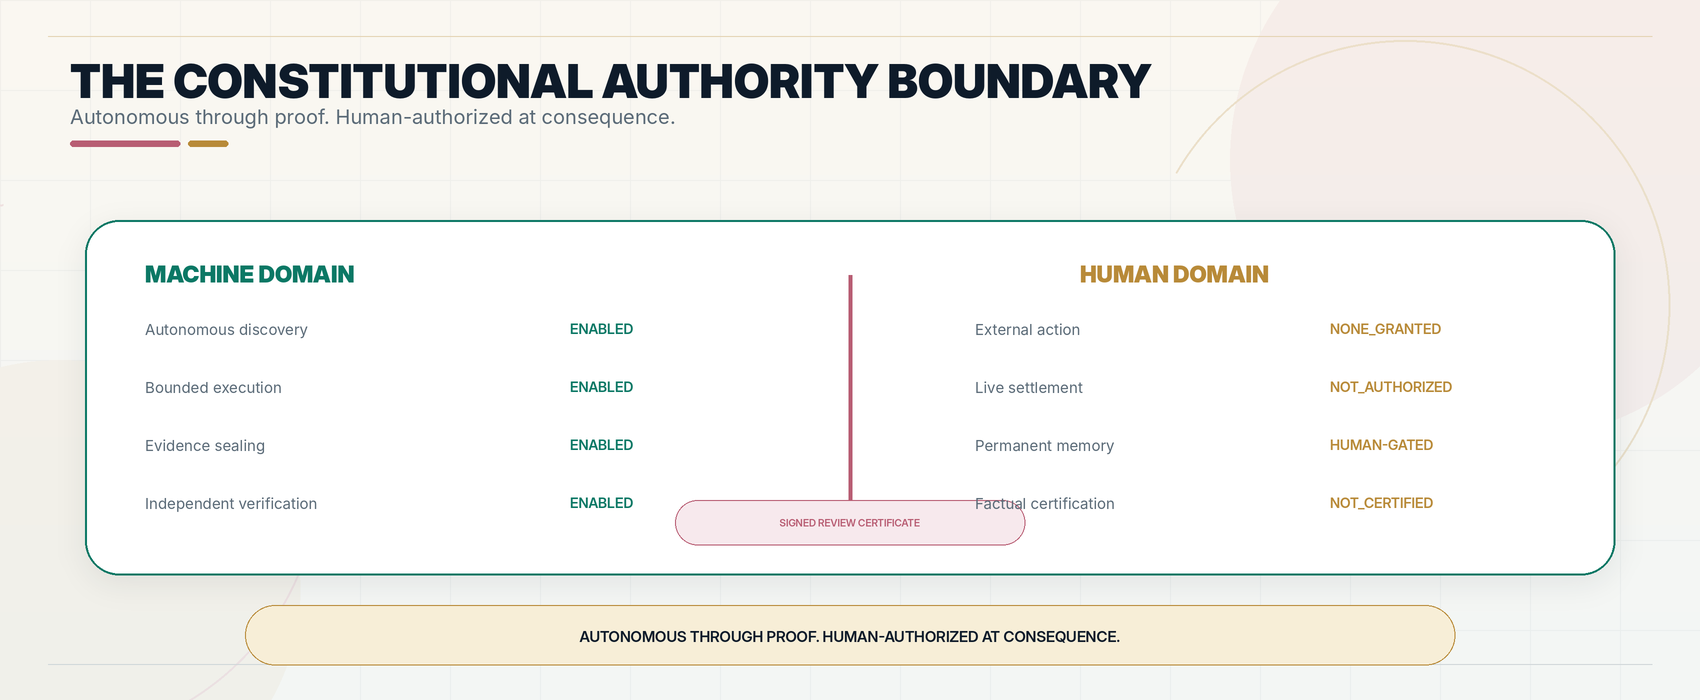
\includegraphics[width=6.75in,height=2.77941in]{media/image12.png}

Figure 11. The public-private proof boundary. Publish the minimum proof
required for trust; keep private intelligence, customer data, and long
traces in controlled storage.

AEP-001 argues: do not put intelligence on-chain; put proof of
intelligence on-chain {[}3{]}. Kernel v3 follows the same boundary
without requiring a chain in the reference implementation. Private
prompts, context, customer documents, raw traces, secret values, and
proprietary workpapers remain outside public proof. Public artifacts can
include content hashes, version roots, signatures, attestations,
selection records, challenge outcomes, and public-safe Evidence Docket
manifests.

\begin{longtable}[]{@{}
  >{\raggedright\arraybackslash}p{(\columnwidth - 2\tabcolsep) * \real{0.5000}}
  >{\raggedright\arraybackslash}p{(\columnwidth - 2\tabcolsep) * \real{0.5000}}@{}}
\toprule\noalign{}
\begin{minipage}[b]{\linewidth}\raggedright
\textbf{Public-safe proof}
\end{minipage} & \begin{minipage}[b]{\linewidth}\raggedright
\textbf{Private intelligence}
\end{minipage} \\
\midrule\noalign{}
\endhead
\bottomrule\noalign{}
\endlastfoot
\textbf{Mission and policy commitments} & Private prompts, internal
strategy, sensitive context \\
\textbf{Artifact IDs, hashes, roots, and public keys} & Raw customer
data, long traces, sensitive tool output \\
\textbf{Validation and review attestations} & Private evaluation
datasets and workpapers \\
\textbf{Selection, challenge, rollout, and rollback receipts} &
Privileged approvals, incident details, trade secrets \\
\textbf{Public-safe Evidence Docket manifest} & Scoped audit appendix
under controlled review \\
\end{longtable}

\subsection{13.1 Chain-agnostic kernel, AEP-compatible
anchoring}\label{chain-agnostic-kernel-aep-compatible-anchoring}

The current kernel is chain-agnostic. A future AEP adapter may anchor
selected commitments, attestations, reputation roots, challenge records,
or review certificates to an on-chain ledger. Such anchoring would
improve shared challengeability and persistence; it would not make the
underlying claim true. On-chain code should enforce rights, scopes, and
settlement conditions, while private intelligence remains off-chain.

\subsection{13.2 Data minimization}\label{data-minimization}

Public proof should reveal the minimum information necessary to verify
integrity, authority, and status. The proof package must avoid leaking
private data through file names, metadata, hashes of low-entropy
secrets, embedded logs, or diagnostic reports. Privacy is not achieved
merely by placing a hash on-chain; source material and threat models
matter.

\section{14. Proof Gradient, evolution, and revocable
memory}\label{proof-gradient-evolution-and-revocable-memory}

Kernel v3 does not stop at a successful run. It records a memory
disposition. This connects the current mission to AEP-001: a result may
become a candidate capability only if evidence, evaluation, scope, risk,
challenge, and review are sufficient {[}3{]}.

\begin{longtable}[]{@{}
  >{\raggedright\arraybackslash}p{(\columnwidth - 0\tabcolsep) * \real{1.0000}}@{}}
\toprule\noalign{}
\begin{minipage}[b]{\linewidth}\raggedright
\textbf{ProofGradient(U) = w\_\allowbreak{}q QualityDelta + w\_\allowbreak{}t Transfer + w\_\allowbreak{}v
VerifiedValue + w\_\allowbreak{}i EvidenceIntegrity - w\_\allowbreak{}c Cost - w\_\allowbreak{}r Risk - w\_\allowbreak{}o
Overhead - w\_\allowbreak{}b RollbackDebt}

(7)
\end{minipage} \\
\midrule\noalign{}
\endhead
\bottomrule\noalign{}
\endlastfoot
\end{longtable}

The score is advisory; the gates are mandatory. A high Proof Gradient
cannot bypass evidence validity, independent evaluation, scope
authorization, challenge rights, rollback readiness, or review. Memory
promotion is therefore a separate decision, not an automatic consequence
of task success.

\subsection{14.1 Capability package}\label{capability-package}

A reusable capability package should contain initiation conditions,
bounded workflow, tool contract, expected evidence, validators, cost
profile, risk class, failure history, lineage, rollback plan, expiry,
and promotion status. Reuse without these fields converts a successful
trace into an ungoverned heuristic.

\subsection{14.2 Recursive improvement}\label{recursive-improvement}

Recursive improvement is permitted only as audited state transition. The
system may generate better institutions, routes, workflows, validators,
or memory candidates, but those descendants must earn promotion through
proof. The core law remains: no proof, no evolution; no eval, no
propagation; no rollback, no release.

\subsection{14.3 Failure memory}\label{failure-memory}

Rejected and failed work is not discarded as noise. It is compressed
into failure memory: invalid assumptions, missing evidence, unsafe
actions, validator gaps, cost overruns, challenge outcomes, and revised
rules. Failure memory reduces repeated proof debt and helps future
missions select safer institutions and better evidence plans.

\section{15. Autonomous publication
law}\label{autonomous-publication-law}

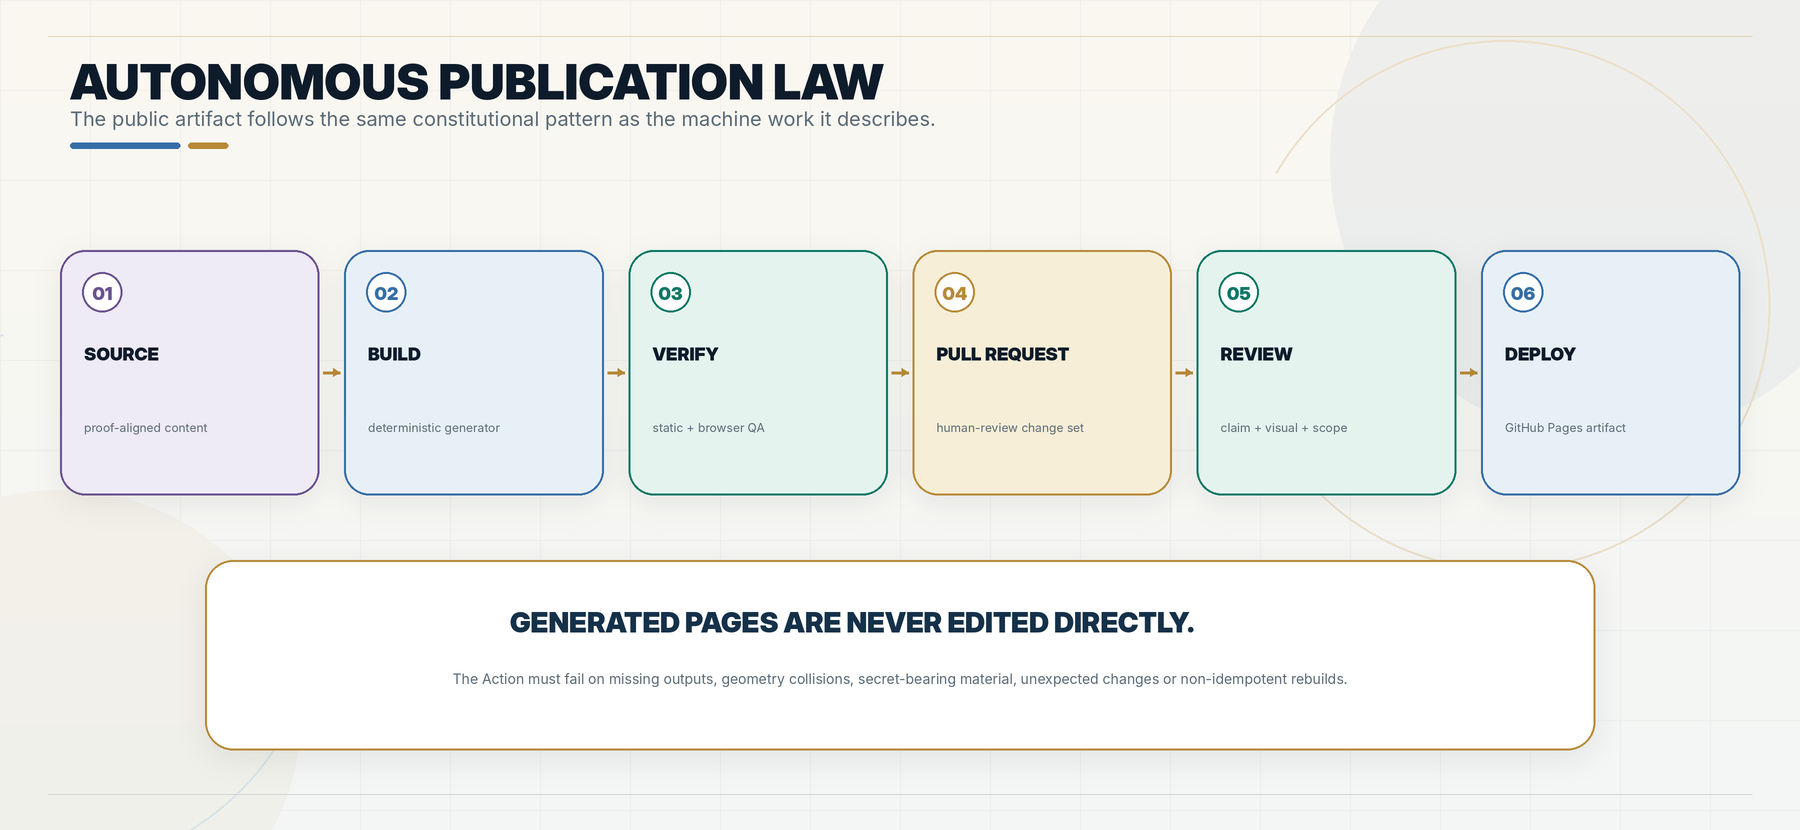
\includegraphics[width=6.75in,height=3.1125in]{media/image13.png}

Figure 12. The autonomous publication law. Source is generated,
verified, reviewed, and deployed; generated live pages are never edited
directly.

The public website is itself an institutional artifact. If it is
hand-edited outside the proof and review process, the communication
layer can drift away from the implementation it describes. Mission OS
therefore introduced an autonomous publication law: proof-aligned source
-\textgreater{} deterministic generator -\textgreater{} QA
-\textgreater{} pull request -\textgreater{} human review
-\textgreater{} publish {[}1{]}.

Kernel v3 strengthens this law. The repository stores source content,
templates, styles, builders, verifiers, and tests. The GitHub Action
builds a temporary site, asserts expected outputs, runs static and
browser QA, verifies geometry and responsive behavior, rejects archives
and secret-bearing material, checks preservation and idempotence,
packages a Pages artifact, and deploys only after gates pass. GitHub
Pages supports custom workflows that upload and deploy a generated Pages
artifact {[}14{]}.

\subsection{15.1 No direct website
update}\label{no-direct-website-update}

The generated site is an output, not a source of truth. Repairs are made
in source templates, content, builder, verifier, or tests. The Action
must reproduce the fix. This prevents one-off production edits,
preserves reviewability, and makes visual regressions part of the
constitutional test suite.

\subsection{15.2 Communication as proof-bearing
infrastructure}\label{communication-as-proof-bearing-infrastructure}

A public artifact is not trustworthy merely because it looks polished.
It becomes infrastructure when its claims, implementation, visual state,
and deployment path are reviewable and replayable. The publication
pipeline is therefore the communication analogue of the kernel state
machine.

\section{16. Security and threat model}\label{security-and-threat-model}

Kernel v3 assumes agents, adapters, users, evaluators, imported bundles,
and operators may be mistaken, adversarial, collusive, or
incentive-misaligned. The security objective is not perfect prevention.
It is fail-closed containment, explicit residual risk, challengeability,
and reversible institutional reliance. This aligns with the NIST AI RMF
emphasis on GOVERN, MAP, MEASURE, and MANAGE across the lifecycle
{[}11,12{]}.

\begin{longtable}[]{@{}
  >{\raggedright\arraybackslash}p{(\columnwidth - 4\tabcolsep) * \real{0.3333}}
  >{\raggedright\arraybackslash}p{(\columnwidth - 4\tabcolsep) * \real{0.3333}}
  >{\raggedright\arraybackslash}p{(\columnwidth - 4\tabcolsep) * \real{0.3333}}@{}}
\toprule\noalign{}
\begin{minipage}[b]{\linewidth}\raggedright
\textbf{Threat}
\end{minipage} & \begin{minipage}[b]{\linewidth}\raggedright
\textbf{Failure mode}
\end{minipage} & \begin{minipage}[b]{\linewidth}\raggedright
\textbf{Control}
\end{minipage} \\
\midrule\noalign{}
\endhead
\bottomrule\noalign{}
\endlastfoot
\textbf{Event tampering} & A payload or prior event is changed after
acceptance. & Payload hashes, predecessor commitments, signatures,
strict replay, mission roots. \\
\textbf{Authority collapse} & One actor proposes, executes, validates,
settles, and authorizes. & Five role keys, transition issuer allowlists,
separate protocol states. \\
\textbf{Silent state mutation} & The interface or storage edits mission
history. & Worker-owned acceptance, append-only Chronicle, rollback as
new event. \\
\textbf{Validator capture} & A verifier colludes or weak validation is
treated as consensus. & Dissent preservation, challenge window, future
quorum and independence profiles. \\
\textbf{Evidence laundering} & Generated artifacts are presented as
external proof. & Explicit HASHED, SIGNED, EXTERNALLY\_\allowbreak{}ATTESTED,
HUMAN\_\allowbreak{}REVIEWED status. \\
\textbf{Replay ambiguity} & Equivalent data serialize differently or
event order is unclear. & Canonical payload rules, logical clock,
predecessor chain, deterministic identifiers. \\
\textbf{Unsafe import} & A malformed or edited mission bundle is
partially trusted. & Schema validation, signature verification, strict
replay, read-only quarantine. \\
\textbf{Premature settlement} & A prepared allocation is mistaken for
live authority. & SettlementIntent carries NONE\_\allowbreak{}GRANTED; activation is
absent and separately governed. \\
\textbf{Key compromise} & A signing key is stolen or misbound to
identity. & Key custody, rotation, revocation, credential binding,
incident events. \\
\textbf{Privacy leakage} & Public proof reveals sensitive prompts, data,
logs, or metadata. & Data minimization, public/private Dockets, secret
scans, scoped audit appendices. \\
\textbf{UI bypass} & The page mutates state or triggers action outside
the worker. & DOM-independent core, worker boundary, no network or
external action APIs. \\
\textbf{Reward hacking} & Adapters optimize proxy scores instead of
institutional value. & Hard gates, negative controls, delayed outcomes,
independent review, falsification tests. \\
\end{longtable}

\subsection{16.1 Default-deny reference
posture}\label{default-deny-reference-posture}

\begin{longtable}[]{@{}
  >{\raggedright\arraybackslash}p{(\columnwidth - 2\tabcolsep) * \real{0.5000}}
  >{\raggedright\arraybackslash}p{(\columnwidth - 2\tabcolsep) * \real{0.5000}}@{}}
\toprule\noalign{}
\begin{minipage}[b]{\linewidth}\raggedright
\textbf{Capability}
\end{minipage} & \begin{minipage}[b]{\linewidth}\raggedright
\textbf{Reference posture}
\end{minipage} \\
\midrule\noalign{}
\endhead
\bottomrule\noalign{}
\endlastfoot
\textbf{External dependencies} & Disabled \\
\textbf{API keys} & Absent \\
\textbf{Wallet connection} & Disabled \\
\textbf{Network reads/writes} & Disabled \\
\textbf{Live model calls} & Disabled \\
\textbf{Live compute} & Disabled \\
\textbf{Live token movement} & Disabled \\
\textbf{Credential issuance} & Disabled \\
\textbf{Automatic memory promotion} & Disabled \\
\textbf{External authority} & NONE\_\allowbreak{}GRANTED \\
\textbf{Storage} & Local append-only IndexedDB Chronicle \\
\textbf{Signature algorithm} & Ed25519 \\
\textbf{Worker isolation} & Enabled \\
\end{longtable}

\subsection{16.2 Security boundary of the reference
release}\label{security-boundary-of-the-reference-release}

Default-deny behavior reduces the immediate action surface but does not
prove production security. Browser implementation, origin security,
supply-chain integrity, dependency management, key persistence,
cross-browser behavior, denial-of-service resistance, secure deletion,
accessibility, and operator procedures remain engineering obligations.
The reference release is a constitutional kernel demonstration, not an
externally audited production security product.

\section{17. Evaluation and benchmark
program}\label{evaluation-and-benchmark-program}

A constitution becomes scientific only when it can fail. The benchmark
program therefore compares the kernel against increasingly strong
baselines and publishes negative controls, rejected candidates, tamper
failures, rollback failures, and delayed outcomes.

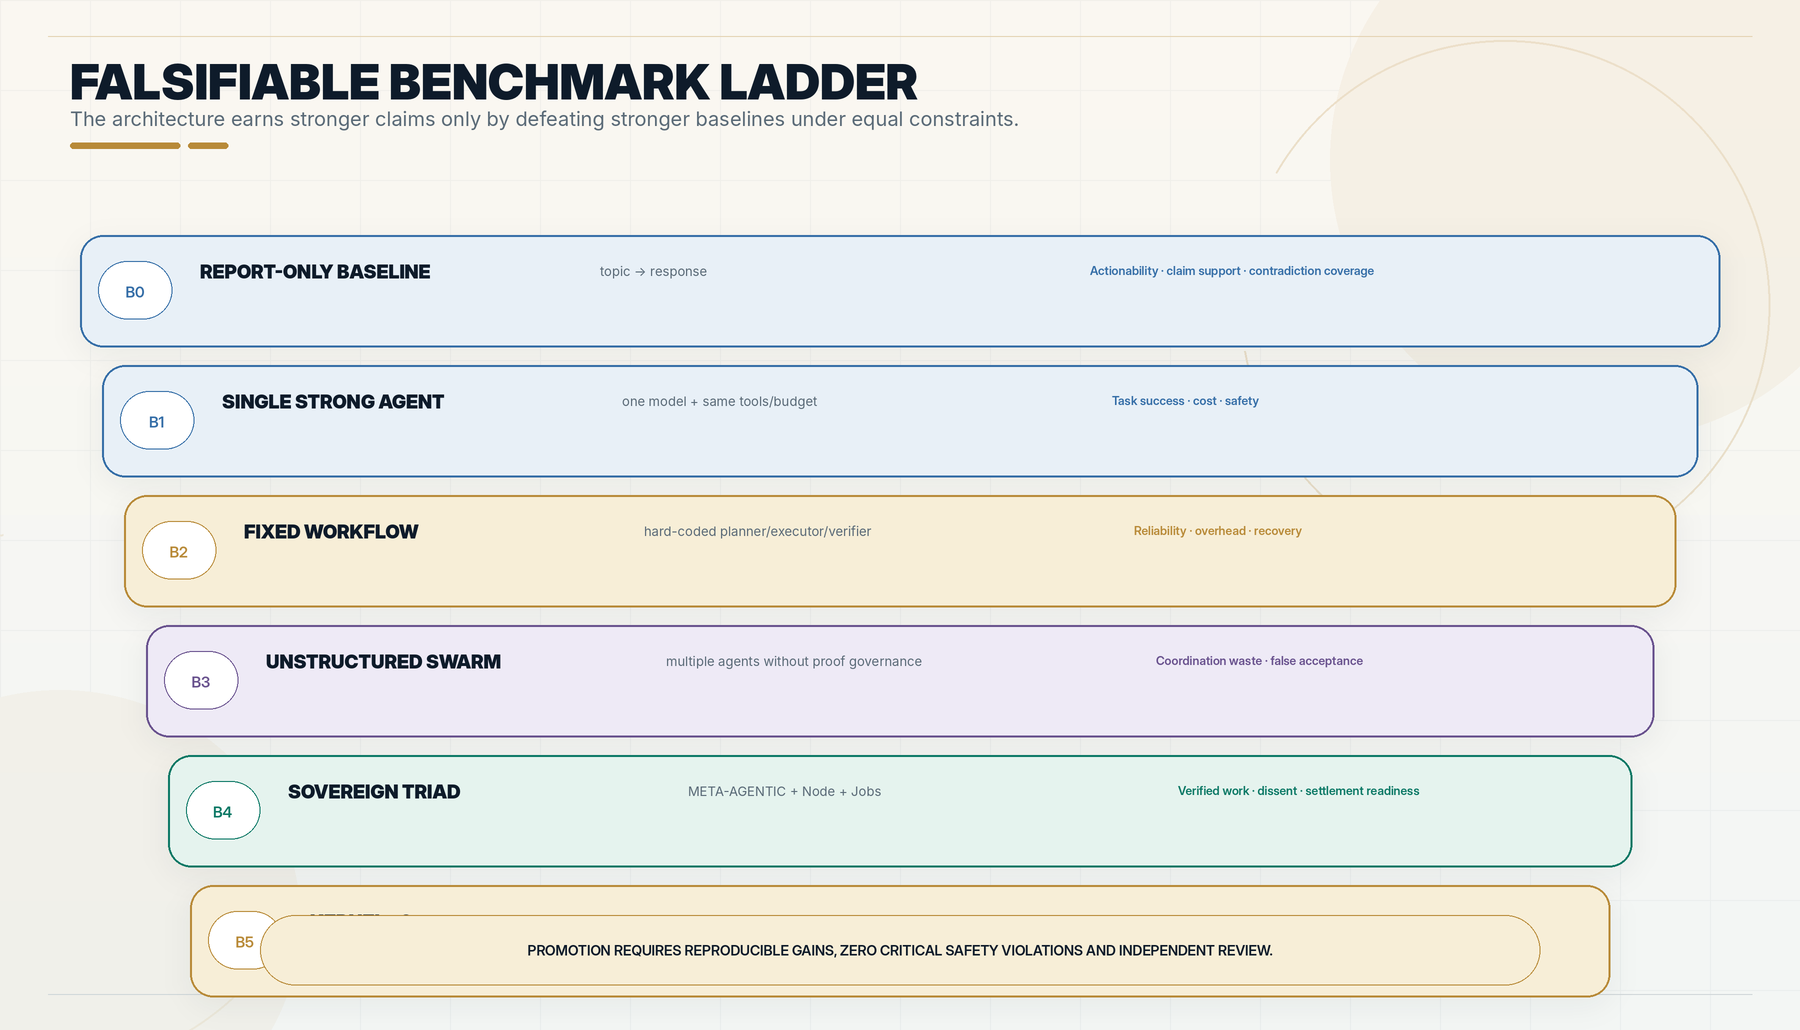
\includegraphics[width=6.75in,height=3.8625in]{media/image14.png}

Figure 13. The falsifiable benchmark ladder, from report-only output to
the signed, replayable, human-gated Kernel v3.

\subsection{17.1 Protocol conformance
tests}\label{protocol-conformance-tests}

\begin{longtable}[]{@{}
  >{\raggedright\arraybackslash}p{(\columnwidth - 4\tabcolsep) * \real{0.3333}}
  >{\raggedright\arraybackslash}p{(\columnwidth - 4\tabcolsep) * \real{0.3333}}
  >{\raggedright\arraybackslash}p{(\columnwidth - 4\tabcolsep) * \real{0.3333}}@{}}
\toprule\noalign{}
\begin{minipage}[b]{\linewidth}\raggedright
\textbf{Test family}
\end{minipage} & \begin{minipage}[b]{\linewidth}\raggedright
\textbf{Question}
\end{minipage} & \begin{minipage}[b]{\linewidth}\raggedright
\textbf{Primary metric}
\end{minipage} \\
\midrule\noalign{}
\endhead
\bottomrule\noalign{}
\endlastfoot
\textbf{Schema and transition} & Are invalid state and envelope
combinations rejected? & Transition rejection precision; illegal advance
rate \\
\textbf{Authority separation} & Can any role sign or advance a forbidden
transition? & Unauthorized acceptance rate; expected 0 \\
\textbf{Tamper and replay} & Does any changed payload, signature,
predecessor, or order fail? & Tamper detection rate; replay
determinism \\
\textbf{Bundle import} & Are malformed or partial imports quarantined? &
Unsafe import acceptance rate; expected 0 \\
\textbf{Dissent and challenge} & Are minority opinions and challenge
windows preserved? & Dissent retention; challenge trace completeness \\
\textbf{Human review} & Can machine-complete work bypass the certificate
boundary? & False permission rate; expected 0 \\
\textbf{Memory promotion} & Can capability memory promote automatically?
& Unauthorized promotion rate; expected 0 \\
\textbf{Publication} & Can source changes create missing, overlapping,
secret-bearing, or non-idempotent pages? & Build failure coverage;
geometry collisions; secret scan \\
\end{longtable}

\subsection{17.2 Real-task benchmark
families}\label{real-task-benchmark-families}

Protocol conformance is necessary but insufficient. Real-task evaluation
should include software repair, evidence-backed research, enterprise
workflow analysis, policy-bound browser or API work, scientific/data
workflows, procurement diligence, and defensive cybersecurity readiness.
Each task should have a public-safe manifest, strong baselines, equal
model/tool/budget constraints, executed artifacts, cost and safety
ledgers, validator reports, replay instructions, and delayed-outcome
checks.

\subsection{17.3 Verified Work Density}\label{verified-work-density}

\begin{longtable}[]{@{}
  >{\raggedright\arraybackslash}p{(\columnwidth - 0\tabcolsep) * \real{1.0000}}@{}}
\toprule\noalign{}
\begin{minipage}[b]{\linewidth}\raggedright
\textbf{D\_\allowbreak{}verified = (VerifiedValue × ProofIntegrity × Replayability ×
PolicyCompliance × Reuse) / (ComputeCost + ToolCost + Latency +
ResidualRisk + GovernanceOverhead)}

(8)
\end{minipage} \\
\midrule\noalign{}
\endhead
\bottomrule\noalign{}
\endlastfoot
\end{longtable}

The metric prevents the system from winning merely by spending more,
adding more agents, or creating more paperwork. Governance overhead is
not assumed to be free. Kernel v3 earns its place only if the reduction
in false acceptance, proof debt, review friction, and repeated work
exceeds the coordination and verification cost it introduces.

\subsection{17.4 Key empirical questions}\label{key-empirical-questions}

\begin{itemize}
\item
  Does Kernel v3 reduce unsupported major claims relative to report-only
  and agent-only baselines?
\item
  Does role separation lower false acceptance and unsafe propagation?
\item
  Does strict replay detect tampering without making ordinary inspection
  impractical?
\item
  Does the Evidence Docket improve reviewer decision readiness and
  reduce review time?
\item
  Does failure memory or capability packaging improve later missions
  under held-out tasks?
\item
  Do production adapters preserve the same authority boundary under real
  network, model, and enterprise integrations?
\item
  Does the system remain useful when independent validators disagree or
  delay?
\item
  Can cross-institutional bundles be verified without exposing private
  intelligence?
\end{itemize}

\section{18. Reference implementation and current
evidence}\label{reference-implementation-and-current-evidence}

The v3.2.0 reference implementation is an executable browser-local
system {[}4{]}. It includes five public surfaces: constitutional mission
theatre, protocol registry, durable Chronicle, independent verifier, and
adapter SDK. The kernel uses deterministic local adapters, WebCrypto
signing, a Web Worker transition boundary, IndexedDB persistence,
exportable mission bundles, strict replay, human review dispositions,
and fail-closed incident paths.

\begin{longtable}[]{@{}
  >{\raggedright\arraybackslash}p{(\columnwidth - 2\tabcolsep) * \real{0.5000}}
  >{\raggedright\arraybackslash}p{(\columnwidth - 2\tabcolsep) * \real{0.5000}}@{}}
\toprule\noalign{}
\begin{minipage}[b]{\linewidth}\raggedright
\textbf{Implementation property}
\end{minipage} & \begin{minipage}[b]{\linewidth}\raggedright
\textbf{Reference release}
\end{minipage} \\
\midrule\noalign{}
\endhead
\bottomrule\noalign{}
\endlastfoot
\textbf{Constitutional states} & 17 \\
\textbf{Typed envelopes} & 10 \\
\textbf{Signing authorities} & 5 \\
\textbf{Replaceable adapters} & 3 \\
\textbf{Adapter methods} & 6 \\
\textbf{Human review dispositions} & 4 \\
\textbf{External actions} & 0 \\
\textbf{Network requests} & 0 \\
\textbf{Wallet connections} & 0 \\
\textbf{Token movements} & 0 \\
\end{longtable}

\subsection{18.1 Internal engineering
validation}\label{internal-engineering-validation}

The source release reports 414/414 static, schema, security, and
preservation checks; 17/17 deterministic unit tests; and 62/62 Chromium
runtime, responsive, and geometry checks. It also reports byte-identical
second builds, zero unexpected file changes, zero browser console
errors, and zero external browser requests {[}4{]}. These results are
internal engineering evidence. They are not independent security review,
factual validation, enterprise reliability, or empirical proof of
superior autonomous work.

\subsection{18.2 What exists and what does
not}\label{what-exists-and-what-does-not}

\begin{longtable}[]{@{}
  >{\raggedright\arraybackslash}p{(\columnwidth - 2\tabcolsep) * \real{0.5000}}
  >{\raggedright\arraybackslash}p{(\columnwidth - 2\tabcolsep) * \real{0.5000}}@{}}
\toprule\noalign{}
\begin{minipage}[b]{\linewidth}\raggedright
\textbf{Exists now}
\end{minipage} & \begin{minipage}[b]{\linewidth}\raggedright
\textbf{Does not yet exist}
\end{minipage} \\
\midrule\noalign{}
\endhead
\bottomrule\noalign{}
\endlastfoot
\textbf{Executable local state machine and worker-owned transition
validation.} & Production authorization service. \\
\textbf{Local role keys and signed events.} & Institutionally bound
identity, enterprise key management, or external credential issuer. \\
\textbf{Append-only local Chronicle and portable bundle replay.} &
Multi-party distributed ledger or independent external archival
guarantee. \\
\textbf{Deterministic META-AGENTIC, Node, and Jobs adapters.} & Live
model, enterprise, node network, or independent evaluator adapters. \\
\textbf{Evidence Docket structure and review certificate.} & External
factual certification, legal approval, or regulated reliance. \\
\textbf{Autonomous source-to-Pages build with QA.} & Proof that all
future workflows or browsers are defect-free. \\
\end{longtable}

\subsection{18.3 Evidence ladder}\label{evidence-ladder}

\begin{longtable}[]{@{}
  >{\raggedright\arraybackslash}p{(\columnwidth - 4\tabcolsep) * \real{0.3333}}
  >{\raggedright\arraybackslash}p{(\columnwidth - 4\tabcolsep) * \real{0.3333}}
  >{\raggedright\arraybackslash}p{(\columnwidth - 4\tabcolsep) * \real{0.3333}}@{}}
\toprule\noalign{}
\begin{minipage}[b]{\linewidth}\raggedright
\textbf{Level}
\end{minipage} & \begin{minipage}[b]{\linewidth}\raggedright
\textbf{Meaning}
\end{minipage} & \begin{minipage}[b]{\linewidth}\raggedright
\textbf{Current status}
\end{minipage} \\
\midrule\noalign{}
\endhead
\bottomrule\noalign{}
\endlastfoot
\textbf{E0} & Doctrine and formal architecture & Achieved \\
\textbf{E1} & Executable local reference and protocol objects &
Achieved \\
\textbf{E2} & Deterministic replay, tamper rejection, and QA & Achieved
internally \\
\textbf{E3} & Authenticated real adapters and external evidence &
Pending \\
\textbf{E4} & Independent evaluator reproduction & Pending \\
\textbf{E5} & Paid production mission portfolio with delayed outcomes &
Pending \\
\textbf{E6} & Cross-institutional interoperability and credential trust
& Pending \\
\textbf{E7} & Neutral standard and settlement network effects &
Strategic horizon \\
\end{longtable}

\section{19. Institutional deployment
doctrine}\label{institutional-deployment-doctrine}

The first deployment should not sell unrestricted autonomy. It should
sell governed improvement: one consequential workflow converted into
mission commitments, bounded execution, Evidence Dockets, independent
evaluation, human review, and rollbackable capability reuse.

\subsection{19.1 Immediate commercial wedge: the proof
mission}\label{immediate-commercial-wedge-the-proof-mission}

A practical offering is a time-bounded proof mission. An institution
supplies one high-stakes objective. GoalOS returns a Governed Decision
State: mission contract, evidence graph, contradictions, verifier
report, risk and cost ledgers, executive brief, decision deck, action
graph, Chronicle entry, and reusable capability package. The value
proposition is not a longer answer. It is a shorter path from
uncertainty to justified action.

\subsection{19.2 Proof-to-Permission API}\label{proof-to-permission-api}

The enterprise product should expose the kernel as a Proof-to-Permission
API: create mission, register identities and authority, run bounded
adapters, attach authenticated evidence, request independent evaluation,
open challenge, prepare review, issue a scoped certificate, export an
audit-ready bundle, and record revocation or memory disposition.

\subsection{19.3 Phased deployment}\label{phased-deployment}

\begin{longtable}[]{@{}
  >{\raggedright\arraybackslash}p{(\columnwidth - 4\tabcolsep) * \real{0.3333}}
  >{\raggedright\arraybackslash}p{(\columnwidth - 4\tabcolsep) * \real{0.3333}}
  >{\raggedright\arraybackslash}p{(\columnwidth - 4\tabcolsep) * \real{0.3333}}@{}}
\toprule\noalign{}
\begin{minipage}[b]{\linewidth}\raggedright
\textbf{Phase}
\end{minipage} & \begin{minipage}[b]{\linewidth}\raggedright
\textbf{Scope}
\end{minipage} & \begin{minipage}[b]{\linewidth}\raggedright
\textbf{Exit criteria}
\end{minipage} \\
\midrule\noalign{}
\endhead
\bottomrule\noalign{}
\endlastfoot
\textbf{0 - Local reference} & Deterministic adapters, browser-local
signing, replay, no external action. & Protocol conformance and failure
injection pass. \\
\textbf{1 - Authenticated evidence pilot} & Read-only enterprise data,
authenticated sources, external evaluator adapter. & Independent replay
and evidence-source audit. \\
\textbf{2 - Bounded enterprise workflow} & One repeatable workflow with
scoped tool writes and human approval. & Measured value, rollback drill,
zero unrecorded consequential actions. \\
\textbf{3 - Multi-institution verification} & Independent verifier
organizations, credential binding, challenge process. & Cross-party
replay and acceptable false-permit rate. \\
\textbf{4 - Settlement-ready network} & Proof-conditioned economic
settlement and reputation under separate authorization. & Legal,
security, market, and governance approval; live pilots with limits. \\
\textbf{5 - Neutral infrastructure} & Cross-model, cross-agent,
cross-enterprise standard. & Interoperability, adoption, durable
evidence/reputation network effects. \\
\end{longtable}

\subsection{19.4 Where the moat can form}\label{where-the-moat-can-form}

The interface and state machine can be reproduced. Durable defensibility
must accumulate in interconnected graphs: evidence, policy, reputation,
authorization, settlement, and capability memory. When institutions rely
on these histories, switching costs are not merely technical. They
include lost provenance, evaluation relationships, credential history,
policy integration, challenge records, and reusable institutional
memory.

\section{20. Quintessential institutional use
cases}\label{quintessential-institutional-use-cases}

Kernel v3 is most valuable where ordinary automation is too weak for the
consequence of the work, yet the objective is structured enough that
evidence, authority, and rollback can be made explicit. The following
use cases are not a feature list. They are institutional operating
patterns in which proof-bearing autonomy can reduce decision latency
without converting model confidence into unearned permission.

\begin{longtable}[]{@{}
  >{\raggedright\arraybackslash}p{(\columnwidth - 0\tabcolsep) * \real{1.0000}}@{}}
\toprule\noalign{}
\begin{minipage}[b]{\linewidth}\raggedright
\textbf{Use-case doctrine.} Use the smallest sufficient control
structure - but never less than the consequence, evidence, and rollback
burden requires.
\end{minipage} \\
\midrule\noalign{}
\endhead
\bottomrule\noalign{}
\endlastfoot
\end{longtable}

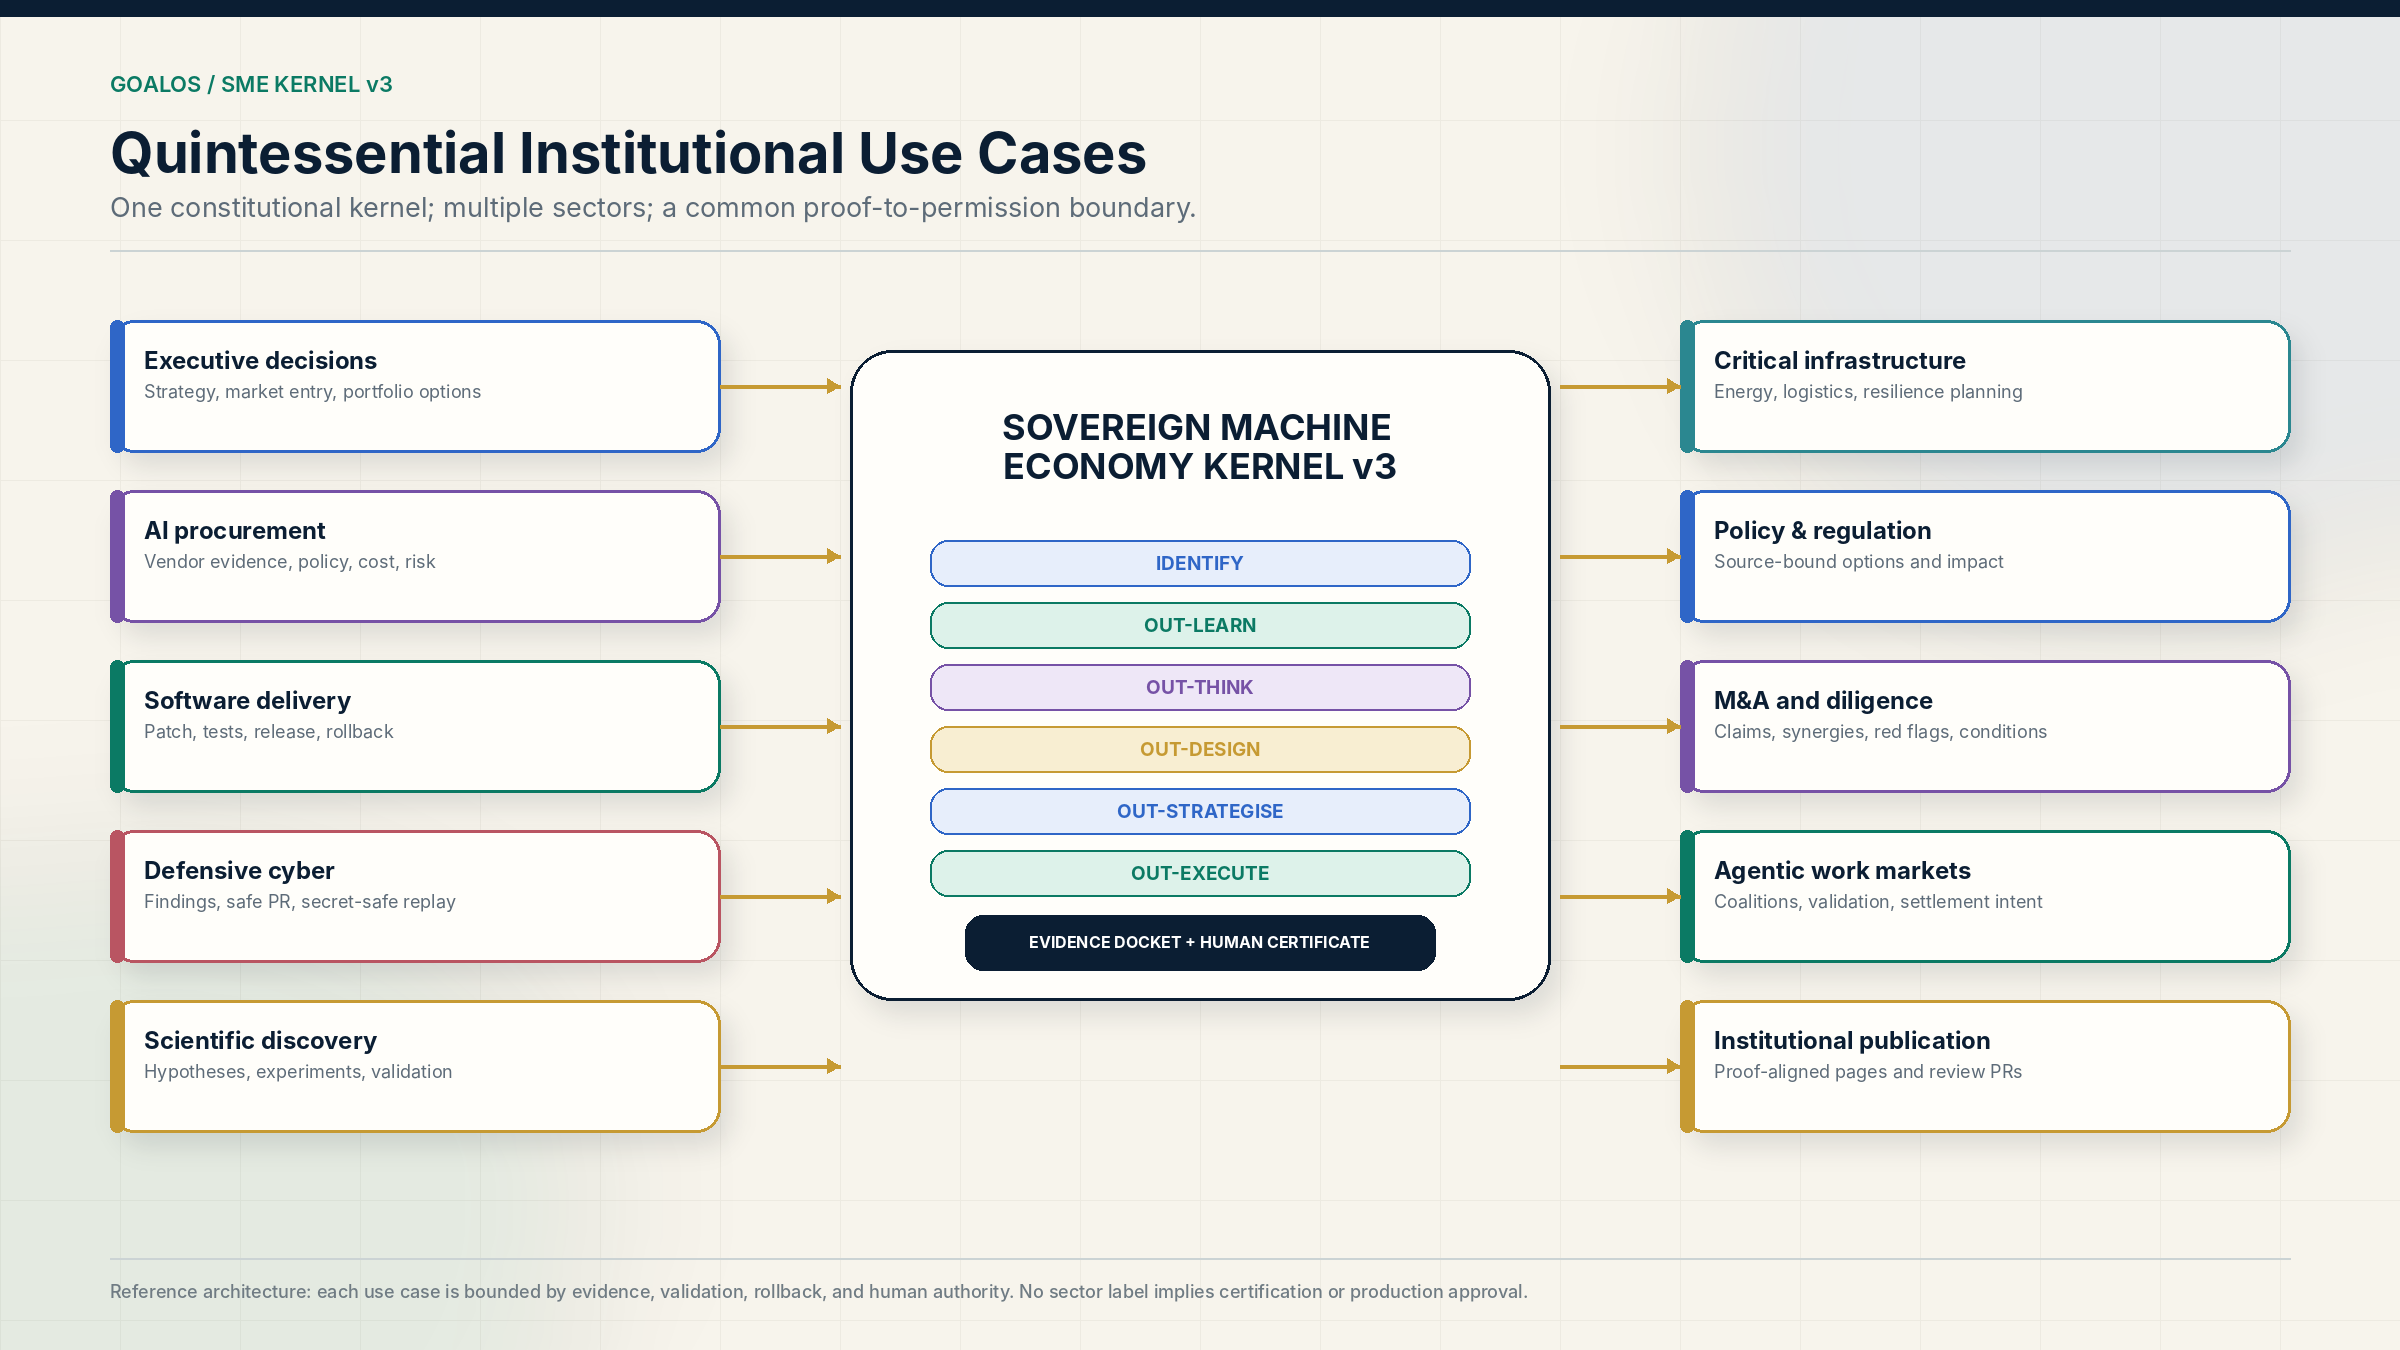
\includegraphics[width=6.75in,height=3.79687in]{media/image15.png}

Figure 15. Quintessential institutional use cases. A single
proof-to-permission kernel can support executive decisions, AI
procurement, software delivery, defensive cybersecurity, scientific
discovery, critical infrastructure, policy, diligence, agentic work
markets, and proof-aligned publication while preserving a common human
authority boundary.

\subsection{20.1 Qualification frontier}\label{qualification-frontier}

Not every task needs a constitutional kernel. A reversible internal
draft may need ordinary automation. A market-entry recommendation needs
a proof mission. A production release, remediation, settlement decision,
or physical intervention requires kernel-governed execution and a
stronger human or institutional certificate. The qualification frontier
is defined by two variables: the intensity of evidence required to
justify reliance, and the consequence or irreversibility of the
contemplated action.

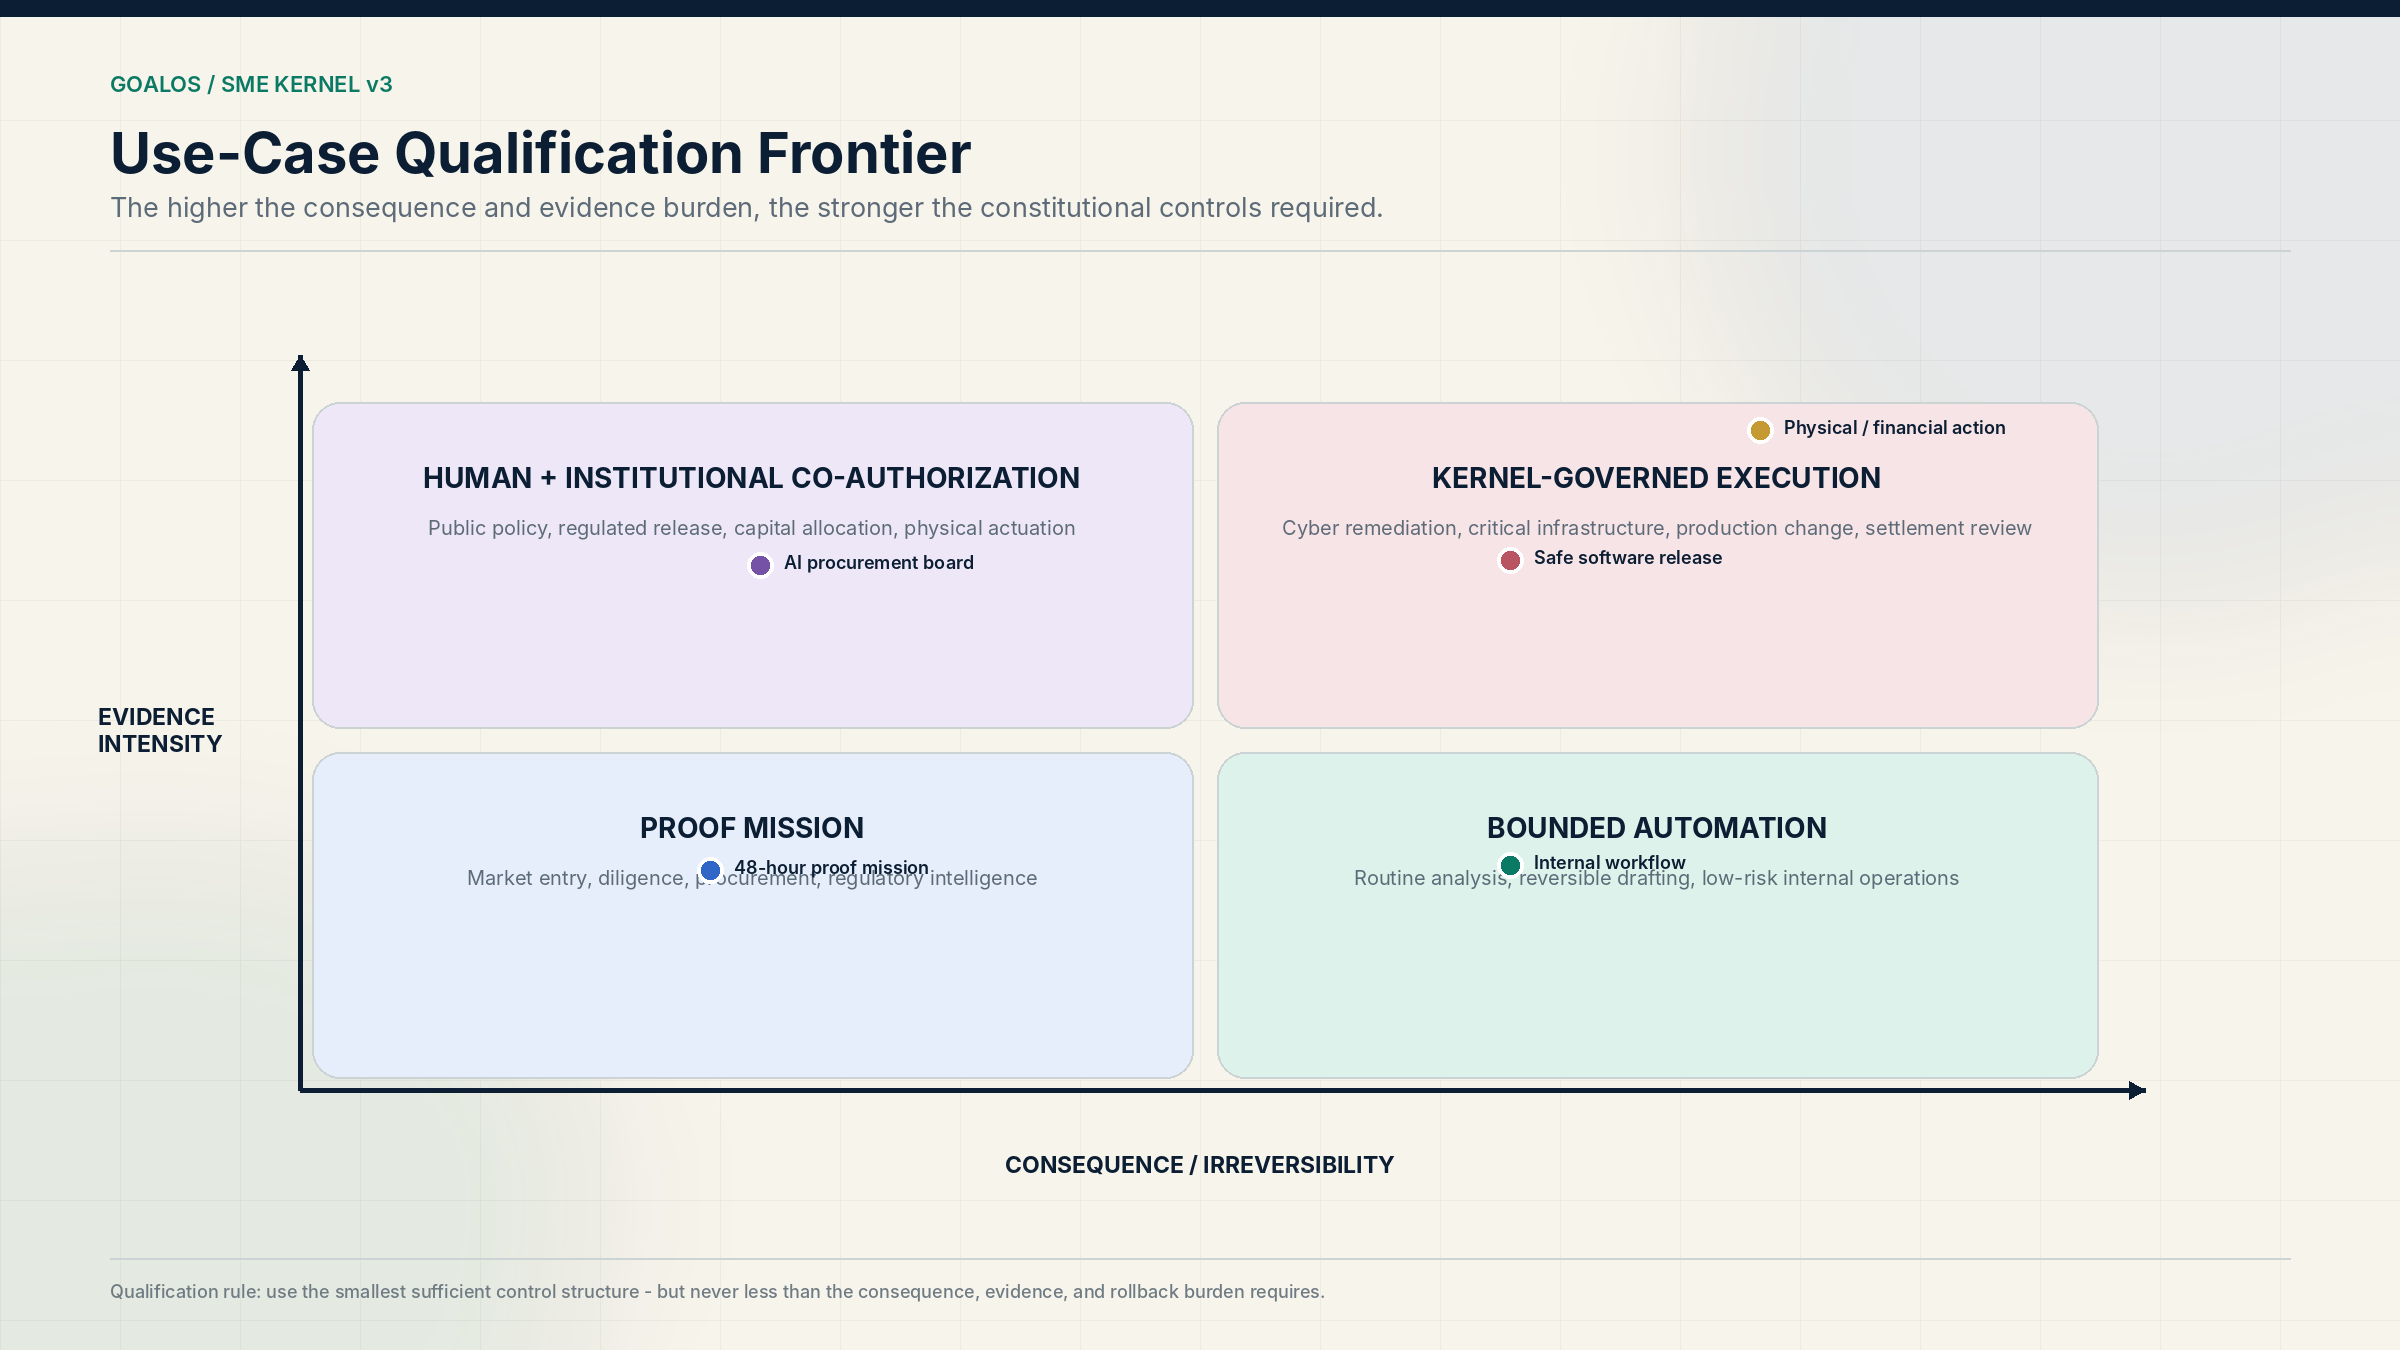
\includegraphics[width=6.75in,height=3.79687in]{media/image16.png}

Figure 16. Use-case qualification frontier. Low-consequence,
low-evidence work may remain bounded automation. As consequence and
evidence burden rise, the system should escalate to proof missions,
kernel-governed execution, and institutional co-authorization.

A mission should be admitted to Kernel v3 when at least one of the
following is true: the result may move capital or production state; the
action affects a regulated or high-trust process; the output is expected
to propagate into future agent behavior; the decision requires competing
sources or models; a rollback or dispute path must exist; or a reviewer
must be able to defend the decision after the original agents are gone.

\begin{longtable}[]{@{}
  >{\raggedright\arraybackslash}p{(\columnwidth - 8\tabcolsep) * \real{0.2000}}
  >{\raggedright\arraybackslash}p{(\columnwidth - 8\tabcolsep) * \real{0.2000}}
  >{\raggedright\arraybackslash}p{(\columnwidth - 8\tabcolsep) * \real{0.2000}}
  >{\raggedright\arraybackslash}p{(\columnwidth - 8\tabcolsep) * \real{0.2000}}
  >{\raggedright\arraybackslash}p{(\columnwidth - 8\tabcolsep) * \real{0.2000}}@{}}
\toprule\noalign{}
\begin{minipage}[b]{\linewidth}\raggedright
\textbf{Use case}
\end{minipage} & \begin{minipage}[b]{\linewidth}\raggedright
\textbf{Institutional decision or action}
\end{minipage} & \begin{minipage}[b]{\linewidth}\raggedright
\textbf{Minimum evidence package}
\end{minipage} & \begin{minipage}[b]{\linewidth}\raggedright
\textbf{Authority boundary}
\end{minipage} & \begin{minipage}[b]{\linewidth}\raggedright
\textbf{Primary metrics}
\end{minipage} \\
\midrule\noalign{}
\endhead
\bottomrule\noalign{}
\endlastfoot
\textbf{Executive decision intelligence} & Select among consequential
strategic options. & Primary-source map; claims and contradictions;
scenario model; risk and option ledger. & Board or named executive
disposition. & Decision latency; claim support; scenario robustness;
unresolved-risk visibility. \\
\textbf{AI procurement and vendor authorization} & Approve, restrict,
pilot, or reject an AI system for a defined workflow. & Equal-budget
task runs; data boundary; security and policy evidence; cost and
reliability ledger. & Procurement, risk, legal, security, and business
owner. & Replay rate; policy-pass rate; false acceptance; total cost;
exit readiness. \\
\textbf{Autonomous software delivery} & Propose and validate a patch or
release candidate. & Diff; tests; dependency and provenance records;
rollout plan; rollback target. & Human merge and deployment authority. &
Test pass; regression rate; change-failure rate; rollback readiness;
review time. \\
\textbf{Defensive cybersecurity remediation} & Turn a defensive finding
into a safe, reviewable remediation. & Finding evidence; minimal patch;
secret-safe logs; policy checks; incident and rollback record. & Human
security and repository owner. & Finding validity; secret leakage=0;
external scans=0; replay; safe PR acceptance. \\
\textbf{Scientific discovery and experimental design} & Prioritize
hypotheses and design falsifiable experiments. & Literature provenance;
contradiction graph; experimental controls; assay plan; uncertainty
ledger. & Scientist, lab, IRB/safety, or domain authority. & Hypothesis
quality; assay reproducibility; negative controls; cost per informative
result. \\
\textbf{Critical infrastructure and energy resilience} & Recommend
bounded interventions for resilience, energy, logistics, or operations.
& Baseline; sensor/model provenance; intervention scenarios;
sensitivity, safety, cost, and rollback. & Asset owner and operating
authority. & Baseline fidelity; scenario sensitivity; pilot safety;
measured outcome; recovery time. \\
\textbf{Policy and regulatory mission operations} & Compare policy
options and implementation consequences. & Primary law and guidance;
stakeholder map; impact scenarios; dissent and claim boundary. &
Authorized public or institutional decision-maker. & Source freshness;
contradiction coverage; distributional impact visibility; review
trace. \\
\textbf{M\&A, partnership, and investment diligence} & Test strategic
claims, dependencies, synergies, and failure conditions. & Claim matrix;
source room; red flags; counterfactuals; integration and
value-realization conditions. & Investment committee or transaction
authority. & Unsupported-claim reduction; risk discovery; option value;
condition coverage; decision speed. \\
\textbf{Proof-gated agentic work market} & Commission, execute,
validate, challenge, and prepare settlement for machine labor. &
Identity; job charter; coalition record; receipts; validator opinions;
dispute and allocation intent. & Human settlement authority or governed
contract boundary. & Proof completeness; validator independence; dispute
rate; contribution fidelity; settlement latency. \\
\textbf{Autonomous publication and institutional communication} &
Generate public artifacts from proof-aligned source without direct
website editing. & Source lineage; deterministic build; link and claim
QA; visual regression; human-review PR. & Human publication reviewer. &
Broken links=0; unsupported claims=0; visual defects=0; provenance
completeness. \\
\end{longtable}

Table 8. Quintessential use-case portfolio. The same kernel contract is
applied differently by domain, but every use case specifies minimum
evidence, authority, metrics, and a fail-closed path.

\subsection{20.2 Strategy, diligence, and capital
allocation}\label{strategy-diligence-and-capital-allocation}

Executive decision intelligence is the most immediate proof-mission
wedge. A strategic question is decomposed into evidence workstreams,
option models, contradiction checks, risk, and action sequencing. The
output is not a recommendation alone; it is a governed option portfolio
that shows which claims are supported, which assumptions dominate the
result, and what must be true before action. The same pattern applies to
market entry, product strategy, portfolio allocation, partnership
selection, and board-level scenario planning.

M\&A and investment diligence add a second discipline: the kernel must
distinguish a plausible narrative from a value-realization mechanism.
The Evidence Docket should bind claimed synergies to dependencies,
integration conditions, counterfactuals, downside paths, and decision
rights. A transaction is not made safe by more analysis; it becomes more
governable when the conditions under which the thesis fails are
explicit.

\subsection{20.3 Procurement, policy, and regulated
adoption}\label{procurement-policy-and-regulated-adoption}

AI procurement is a quintessential proof-to-permission problem. Vendor
claims, model cards, security documents, contractual assurances, and
benchmark scores are inputs, not permission. Kernel v3 can convert a
procurement objective into an equal-budget evaluation portfolio,
data-boundary review, policy test suite, cost ledger, failure analysis,
and exit plan. The Human Review Certificate can scope a pilot to a
workflow, tenant, risk class, duration, and monitoring obligation
without declaring the system generally safe.

Policy and regulatory missions require an even stronger public-private
boundary. Primary law, official guidance, enforcement history,
stakeholder evidence, and distributional impact should remain separable
from interpretation and recommendation. Dissent should be preserved
rather than compressed away. The output is a reviewable policy option
set, not legal advice or autonomous public authority.

\subsection{20.4 Software, cybersecurity, and operational
change}\label{software-cybersecurity-and-operational-change}

Software delivery is a natural fit because acceptance can be grounded in
executable evidence: a patch, tests, static analysis, provenance,
dependency records, rollout scope, monitoring conditions, and rollback.
The kernel can allow broad autonomy in diagnosis and proposal while
withholding merge and deployment authority. This converts agentic coding
from conversational output into a change-control artifact.

Defensive cybersecurity remediation uses the same architecture with
stricter negative permissions. The mission may inspect repository-owned
evidence, identify defensive findings, generate a minimal patch, run
tests, and open a human-review pull request. It may not scan external
targets, expose secret values, generate offensive payloads, auto-merge,
or claim security certification. These are not policy suggestions; they
are hard acceptance guards.

\subsection{20.5 Science, infrastructure, and
resilience}\label{science-infrastructure-and-resilience}

Scientific work becomes proof-bearing when the system preserves the
difference between literature evidence, computational proxy,
experimental plan, executed assay, and externally reproduced result.
Kernel v3 can accelerate search, contradiction mapping, hypothesis
generation, counterfactual design, and experiment planning; it cannot
promote a scientific claim beyond the evidence-contact level actually
achieved.

Critical-infrastructure missions follow a similar ladder. Historical
data and simulation may justify a bounded pilot, but they do not certify
site performance. A resilience or energy mission should emit a baseline
model, intervention set, sensitivity analysis, cost and safety ledger,
pilot criteria, measurement plan, authority map, and rollback. The
institutional gain is a faster path from uncertainty to a safe
experiment - not an unearned claim of real-world savings.

\subsection{20.6 Machine-economy coordination and capability
memory}\label{machine-economy-coordination-and-capability-memory}

AGI Jobs turns mission demand into a governed market: institutions bid,
a coalition is selected, nodes execute, evidence is sealed, validators
commit and reveal opinions, dissent is preserved, challenges are
resolved, and a settlement intent is prepared. Kernel v3 supplies the
authority firewall that prevents market activity from collapsing into
automatic permission. In the reference implementation, settlement
remains an intent object with zero live token movement.

Capability memory is the compounding layer. Accepted methods, workflows,
evidence templates, failure modes, and rollback procedures may become
revocable capability packages with initiation conditions, scope, expiry,
lineage, and promotion authority. The point is not to remember every
output; it is to retain only what earned the right to influence future
work.

\subsection{20.7 Autonomous publication and institutional
communication}\label{autonomous-publication-and-institutional-communication}

Communication is itself a consequential workflow when public pages,
investor materials, technical papers, policy briefs, or audit records
become institutional reality. The autonomous publication law requires
proof-aligned source, deterministic generation, structural and visual
QA, a human-review pull request, and deployment only after review. The
generated artifact must preserve claim boundaries, source lineage, and
rollback. A polished page without that chain is theater; a replayable
page is infrastructure.

\section{21. Institutional reference case
studies}\label{institutional-reference-case-studies}

\begin{longtable}[]{@{}
  >{\raggedright\arraybackslash}p{(\columnwidth - 0\tabcolsep) * \real{1.0000}}@{}}
\toprule\noalign{}
\begin{minipage}[b]{\linewidth}\raggedright
\textbf{Case-study boundary.} The following are worked reference
scenarios. They are designed to be useful, falsifiable, and
implementation-ready, but they are not customer testimonials, external
audits, production certifications, or claims that the described outcomes
have occurred.
\end{minipage} \\
\midrule\noalign{}
\endhead
\bottomrule\noalign{}
\endlastfoot
\end{longtable}

Each case study uses the same anatomy: objective, mission contract,
institution, bounded execution, evidence docket, challenge, human
certificate, and revocable memory. This common structure lets
executives, engineers, auditors, and partners compare radically
different domains without losing the constitutional invariant.

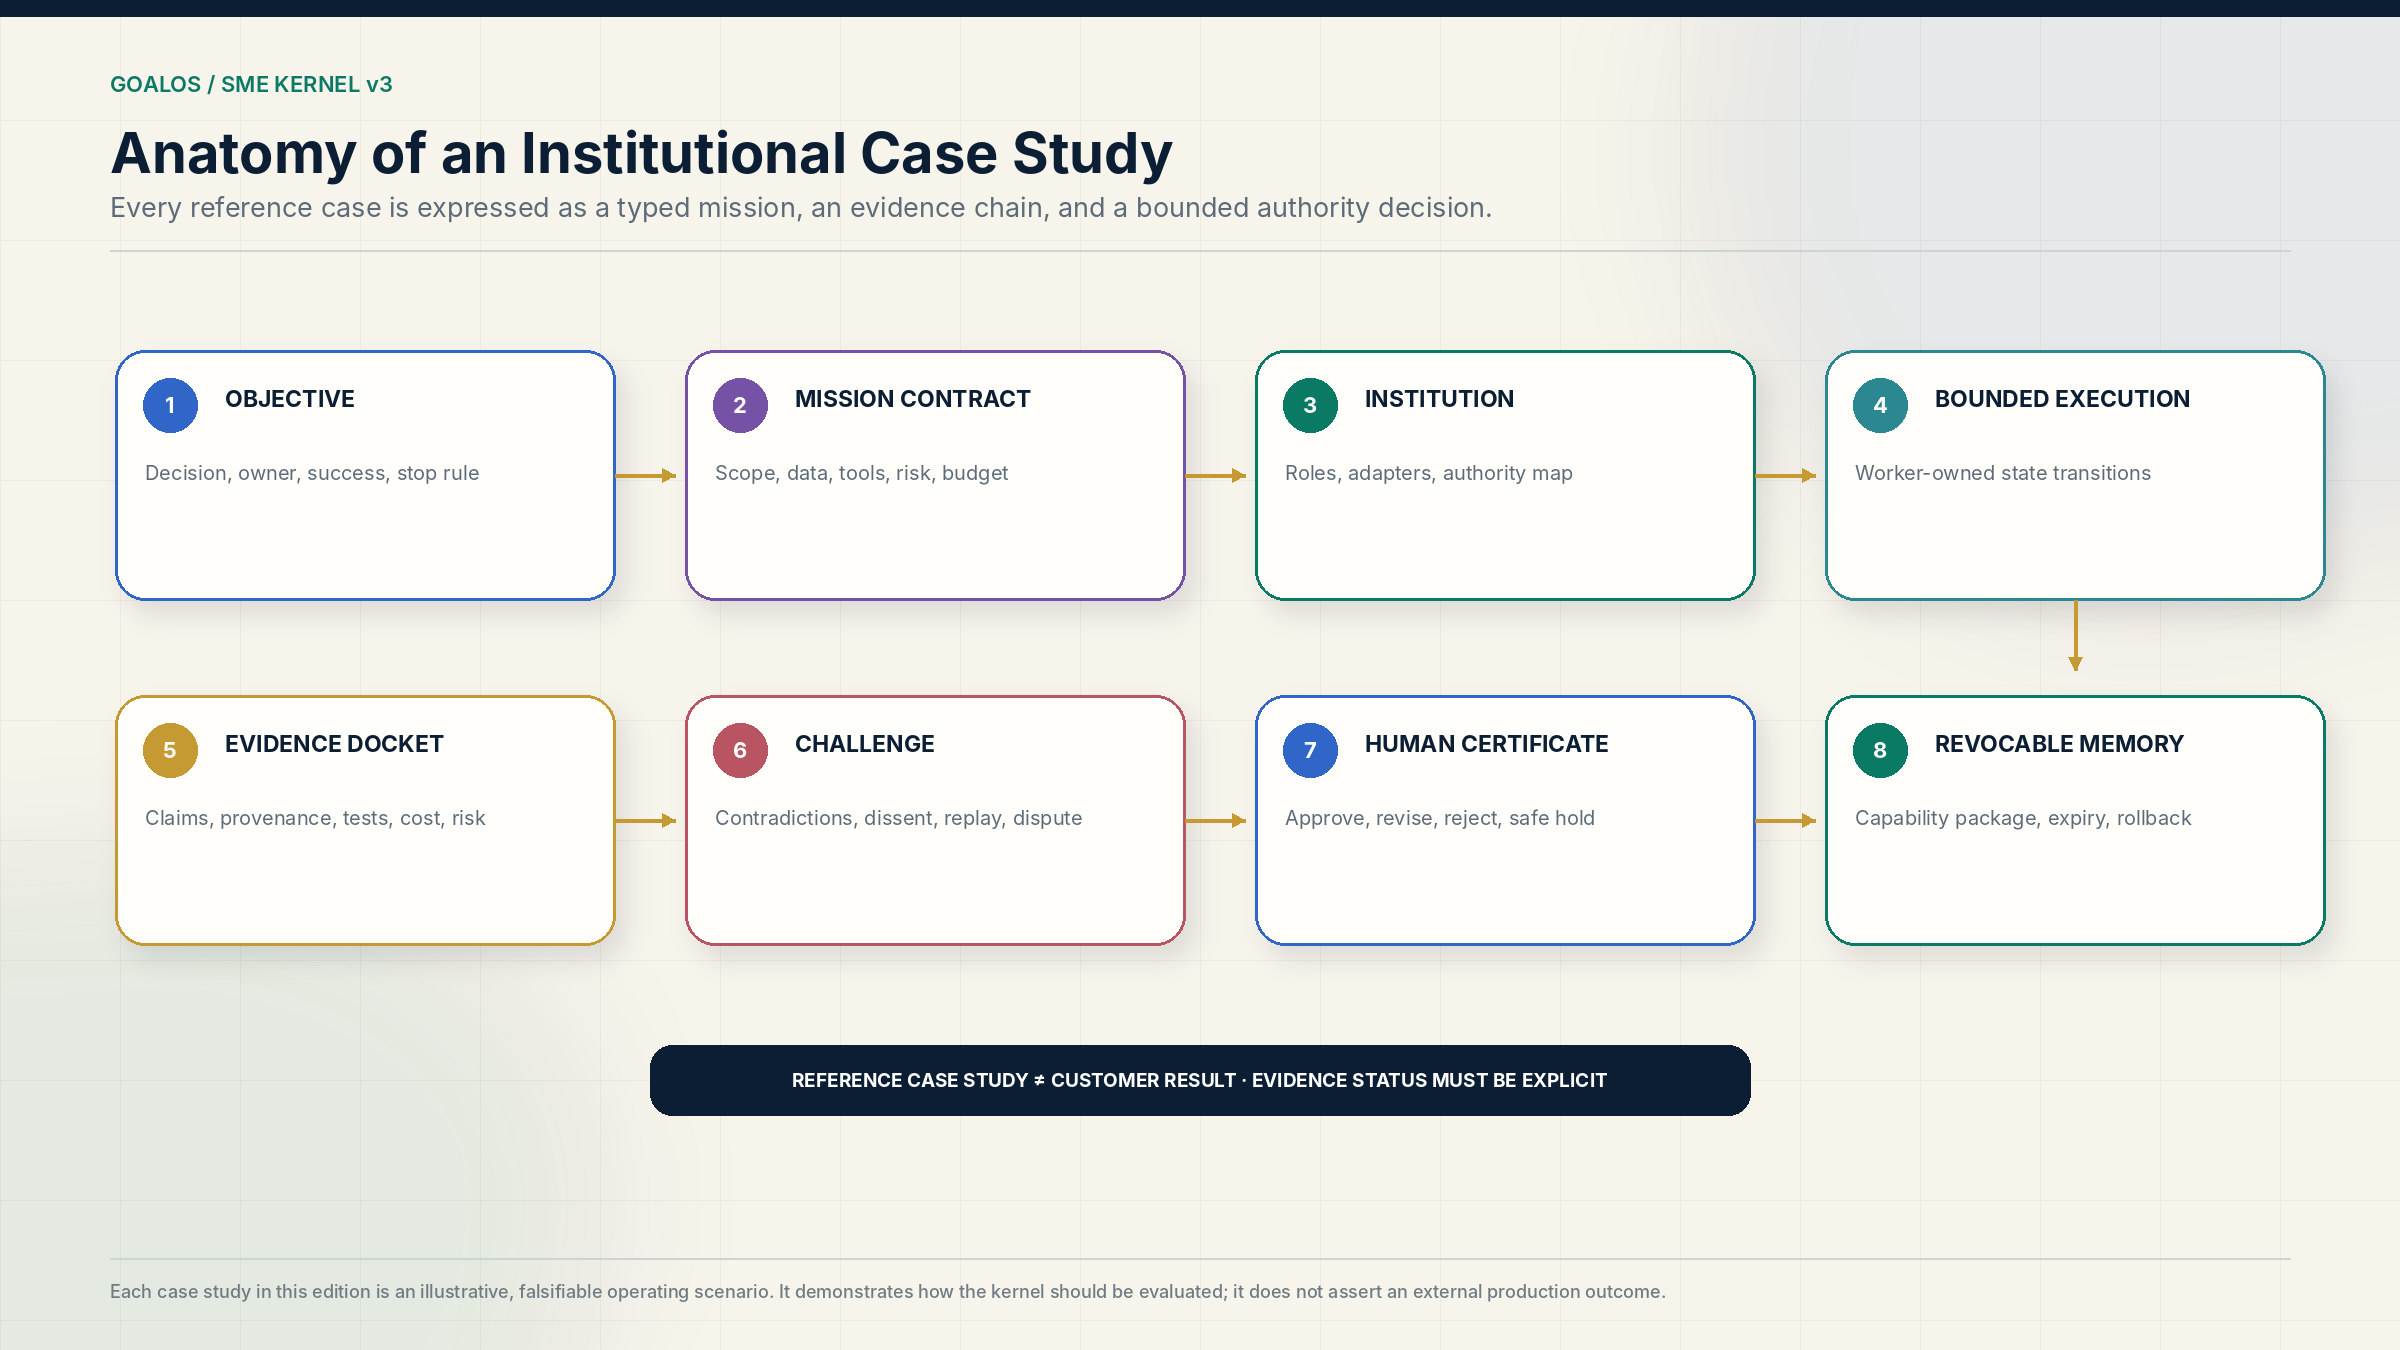
\includegraphics[width=6.75in,height=3.79687in]{media/image17.png}

Figure 17. Anatomy of an institutional case study. Every case is
represented as a typed mission and evidence chain, not as a promotional
narrative. Evidence status and human authority remain explicit.

\begin{longtable}[]{@{}
  >{\raggedright\arraybackslash}p{(\columnwidth - 6\tabcolsep) * \real{0.2500}}
  >{\raggedright\arraybackslash}p{(\columnwidth - 6\tabcolsep) * \real{0.2500}}
  >{\raggedright\arraybackslash}p{(\columnwidth - 6\tabcolsep) * \real{0.2500}}
  >{\raggedright\arraybackslash}p{(\columnwidth - 6\tabcolsep) * \real{0.2500}}@{}}
\toprule\noalign{}
\begin{minipage}[b]{\linewidth}\raggedright
\textbf{Reference case}
\end{minipage} & \begin{minipage}[b]{\linewidth}\raggedright
\textbf{Decision supported}
\end{minipage} & \begin{minipage}[b]{\linewidth}\raggedright
\textbf{Terminal state}
\end{minipage} & \begin{minipage}[b]{\linewidth}\raggedright
\textbf{Core evidence}
\end{minipage} \\
\midrule\noalign{}
\endhead
\bottomrule\noalign{}
\endlastfoot
\textbf{48-hour market-entry proof mission} & Select a launch market and
90-day entry path. & HUMAN\_\allowbreak{}REVIEW\_\allowbreak{}REQUIRED & Claims and contradiction
matrix; option portfolio; risk ledger; action graph. \\
\textbf{Mission-critical AI procurement gate} & Approve, restrict,
pilot, or reject a vendor for one workflow. & HUMAN\_\allowbreak{}REVIEW\_\allowbreak{}REQUIRED &
Equal-budget runs; policy and data boundary; cost, safety, and exit
evidence. \\
\textbf{Defensive remediation and release} & Turn a repo-owned finding
into a tested, rollback-ready PR. & HUMAN\_\allowbreak{}REVIEW\_\allowbreak{}REQUIRED / SAFE\_\allowbreak{}HOLD
& Patch, tests, secret scan, policy checks, release and rollback
plan. \\
\textbf{Cold-chain energy resilience} & Prioritize interventions and
design a measurable pilot. & HUMAN\_\allowbreak{}REVIEW\_\allowbreak{}REQUIRED & Baseline,
intervention scenarios, sensitivity, cost/risk, measurement protocol. \\
\textbf{Scientific experiment design} & Select hypotheses and a
falsifiable experimental sequence. & HUMAN\_\allowbreak{}REVIEW\_\allowbreak{}REQUIRED &
Provenance graph, contradictions, controls, assays, uncertainty and stop
rules. \\
\textbf{Public policy option mission} & Compare policy paths and
implementation consequences. & HUMAN\_\allowbreak{}REVIEW\_\allowbreak{}REQUIRED / DISPUTE\_\allowbreak{}OPEN &
Primary sources, stakeholder evidence, impact model, dissent, legal
boundary. \\
\textbf{Proof-gated agentic work market} & Commission and validate
machine labor; prepare settlement intent. & HUMAN\_\allowbreak{}SETTLEMENT\_\allowbreak{}REVIEW &
Identity, coalition, receipts, parliament, challenge, allocation
intent. \\
\end{longtable}

Table 9. Reference case-study portfolio. Terminal states are explicit,
and none of the cases grants external authority by itself.

\subsection{21.1 Case Study A - 48-hour market-entry proof
mission}\label{case-study-a---48-hour-market-entry-proof-mission}

Mission. An executive team must decide which of several markets should
receive the first launch, which entry mode should be used, and which
conditions would invalidate the recommendation. The deadline is
forty-eight hours; source freshness, regulatory exposure, partner
dependency, and execution capacity are material.

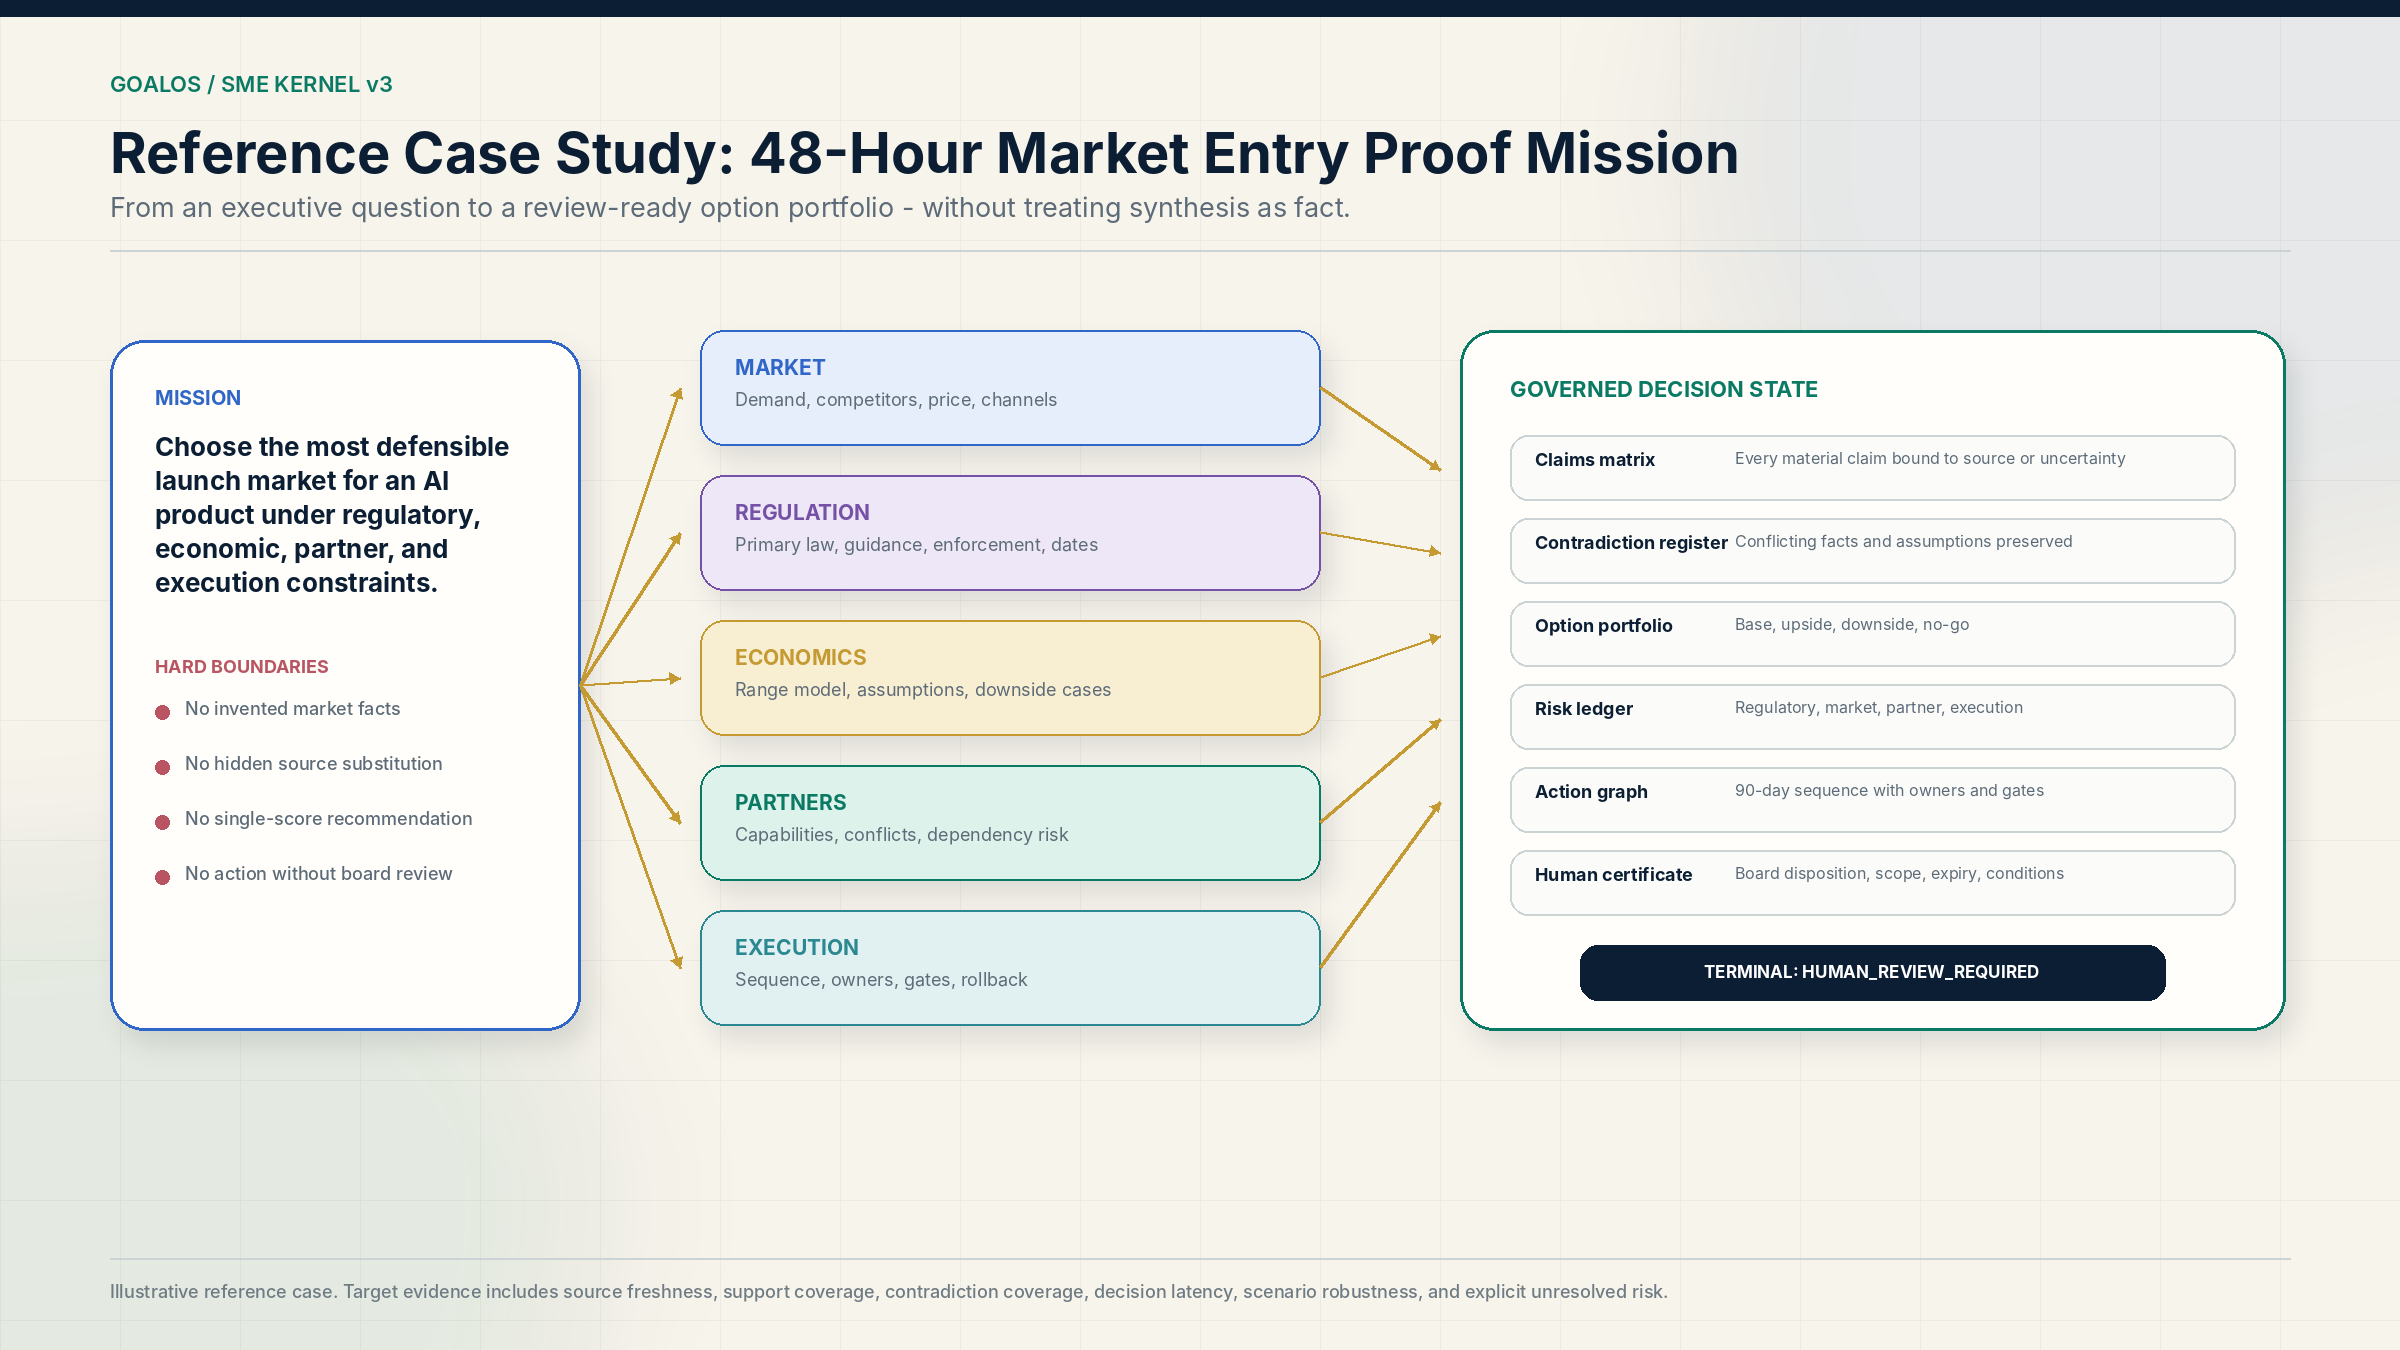
\includegraphics[width=6.75in,height=3.79687in]{media/image18.png}

Figure 18. Reference Case Study A: market-entry proof mission. Parallel
evidence workstreams converge into a Governed Decision State and a
board-review certificate rather than a single opaque score.

\begin{longtable}[]{@{}
  >{\raggedright\arraybackslash}p{(\columnwidth - 2\tabcolsep) * \real{0.5000}}
  >{\raggedright\arraybackslash}p{(\columnwidth - 2\tabcolsep) * \real{0.5000}}@{}}
\toprule\noalign{}
\begin{minipage}[b]{\linewidth}\raggedright
\textbf{Case element}
\end{minipage} & \begin{minipage}[b]{\linewidth}\raggedright
\textbf{Reference implementation}
\end{minipage} \\
\midrule\noalign{}
\endhead
\bottomrule\noalign{}
\endlastfoot
\textbf{Mission contract} & Decision owner, candidate markets, success
criteria, prohibited assumptions, source cutoff, budget, review
deadline, and no-action boundary. \\
\textbf{Institution formed} & Market analyst, regulatory mapper,
economic modeler, partner analyst, execution strategist, contradiction
reviewer, and verifier. \\
\textbf{Evidence produced} & Primary-source register, claim support
matrix, regulatory timeline, scenario economics, partner dependency map,
contradiction register, risk ledger, option portfolio, and 90-day action
graph. \\
\textbf{Challenge path} & A shadow institution must construct the
strongest no-go case and identify the assumptions with the highest
decision sensitivity. \\
\textbf{Human certificate} & The board may approve deliberation, request
revision, open a dispute, or reject to safe hold. The certificate scopes
the decision, expiration, unresolved risks, and conditions precedent. \\
\textbf{Success metrics} & Material-claim support, source freshness,
contradiction coverage, assumption sensitivity, decision latency,
reviewer comprehension, and action-condition completeness. \\
\textbf{Falsification} & The case fails if the recommendation changes
materially under reasonable assumptions, major claims lack primary
evidence, contradictions are hidden, or the option portfolio cannot
explain why alternatives were rejected. \\
\end{longtable}

The reusable capability is not the selected country. It is the verified
market-entry method: source taxonomy, evidence templates, scenario
model, regulatory mapping protocol, partner diligence rubric,
contradiction checks, and reviewer certificate profile. That package may
accelerate the next mission without hard-coding the prior conclusion.

\subsection{21.2 Case Study B - mission-critical AI procurement
gate}\label{case-study-b---mission-critical-ai-procurement-gate}

Mission. An institution is considering three AI systems for a
high-volume, policy-constrained workflow. The procurement committee
needs more than benchmark claims: it needs evidence about data
boundaries, policy compliance, failure recovery, total operating cost,
monitoring, vendor dependency, and exit.

\begin{longtable}[]{@{}
  >{\raggedright\arraybackslash}p{(\columnwidth - 2\tabcolsep) * \real{0.5000}}
  >{\raggedright\arraybackslash}p{(\columnwidth - 2\tabcolsep) * \real{0.5000}}@{}}
\toprule\noalign{}
\begin{minipage}[b]{\linewidth}\raggedright
\textbf{Control}
\end{minipage} & \begin{minipage}[b]{\linewidth}\raggedright
\textbf{What the kernel requires}
\end{minipage} \\
\midrule\noalign{}
\endhead
\bottomrule\noalign{}
\endlastfoot
\textbf{Equal-budget evaluation} & All candidates receive the same task
suite, tool scope, budget, latency target, and acceptance criteria. An
incumbent or no-AI baseline remains visible. \\
\textbf{Evidence boundary} & Vendor documents are separated from
institution-run tests. Unsupported claims remain claims; confidential
materials remain in a private appendix. \\
\textbf{Risk and governance} & Prompt injection, privilege misuse, data
retention, policy drift, model change, outage, auditability, and
human-escalation paths are tested or explicitly marked pending. \\
\textbf{Decision object} & The output is a scoped authorization profile:
reject, sandbox, limited pilot, production candidate, or safe hold -
never a universal declaration that a model is safe. \\
\textbf{Exit readiness} & The package includes exportability, fallback
workflow, contract termination conditions, data deletion evidence, and
operational rollback. \\
\textbf{Success metrics} & Verified task success, policy-pass rate,
false acceptance, human review load, total cost per accepted case,
replay success, incident rate, and switching cost. \\
\end{longtable}

Quintessential result. The committee can explain not only which system
performed best, but which system earned a narrowly scoped right to be
piloted, under which controls, for how long, and with what evidence
burden before expansion.

\subsection{21.3 Case Study C - defensive remediation and rollback-ready
software
release}\label{case-study-c---defensive-remediation-and-rollback-ready-software-release}

Mission. A repository-owned workflow identifies a defensive defect or
release risk. The system may inspect permitted files, propose a minimal
patch, run deterministic checks, package evidence, and open a review
pull request. It may not touch external targets, reveal secrets,
auto-merge, or represent the result as certification.

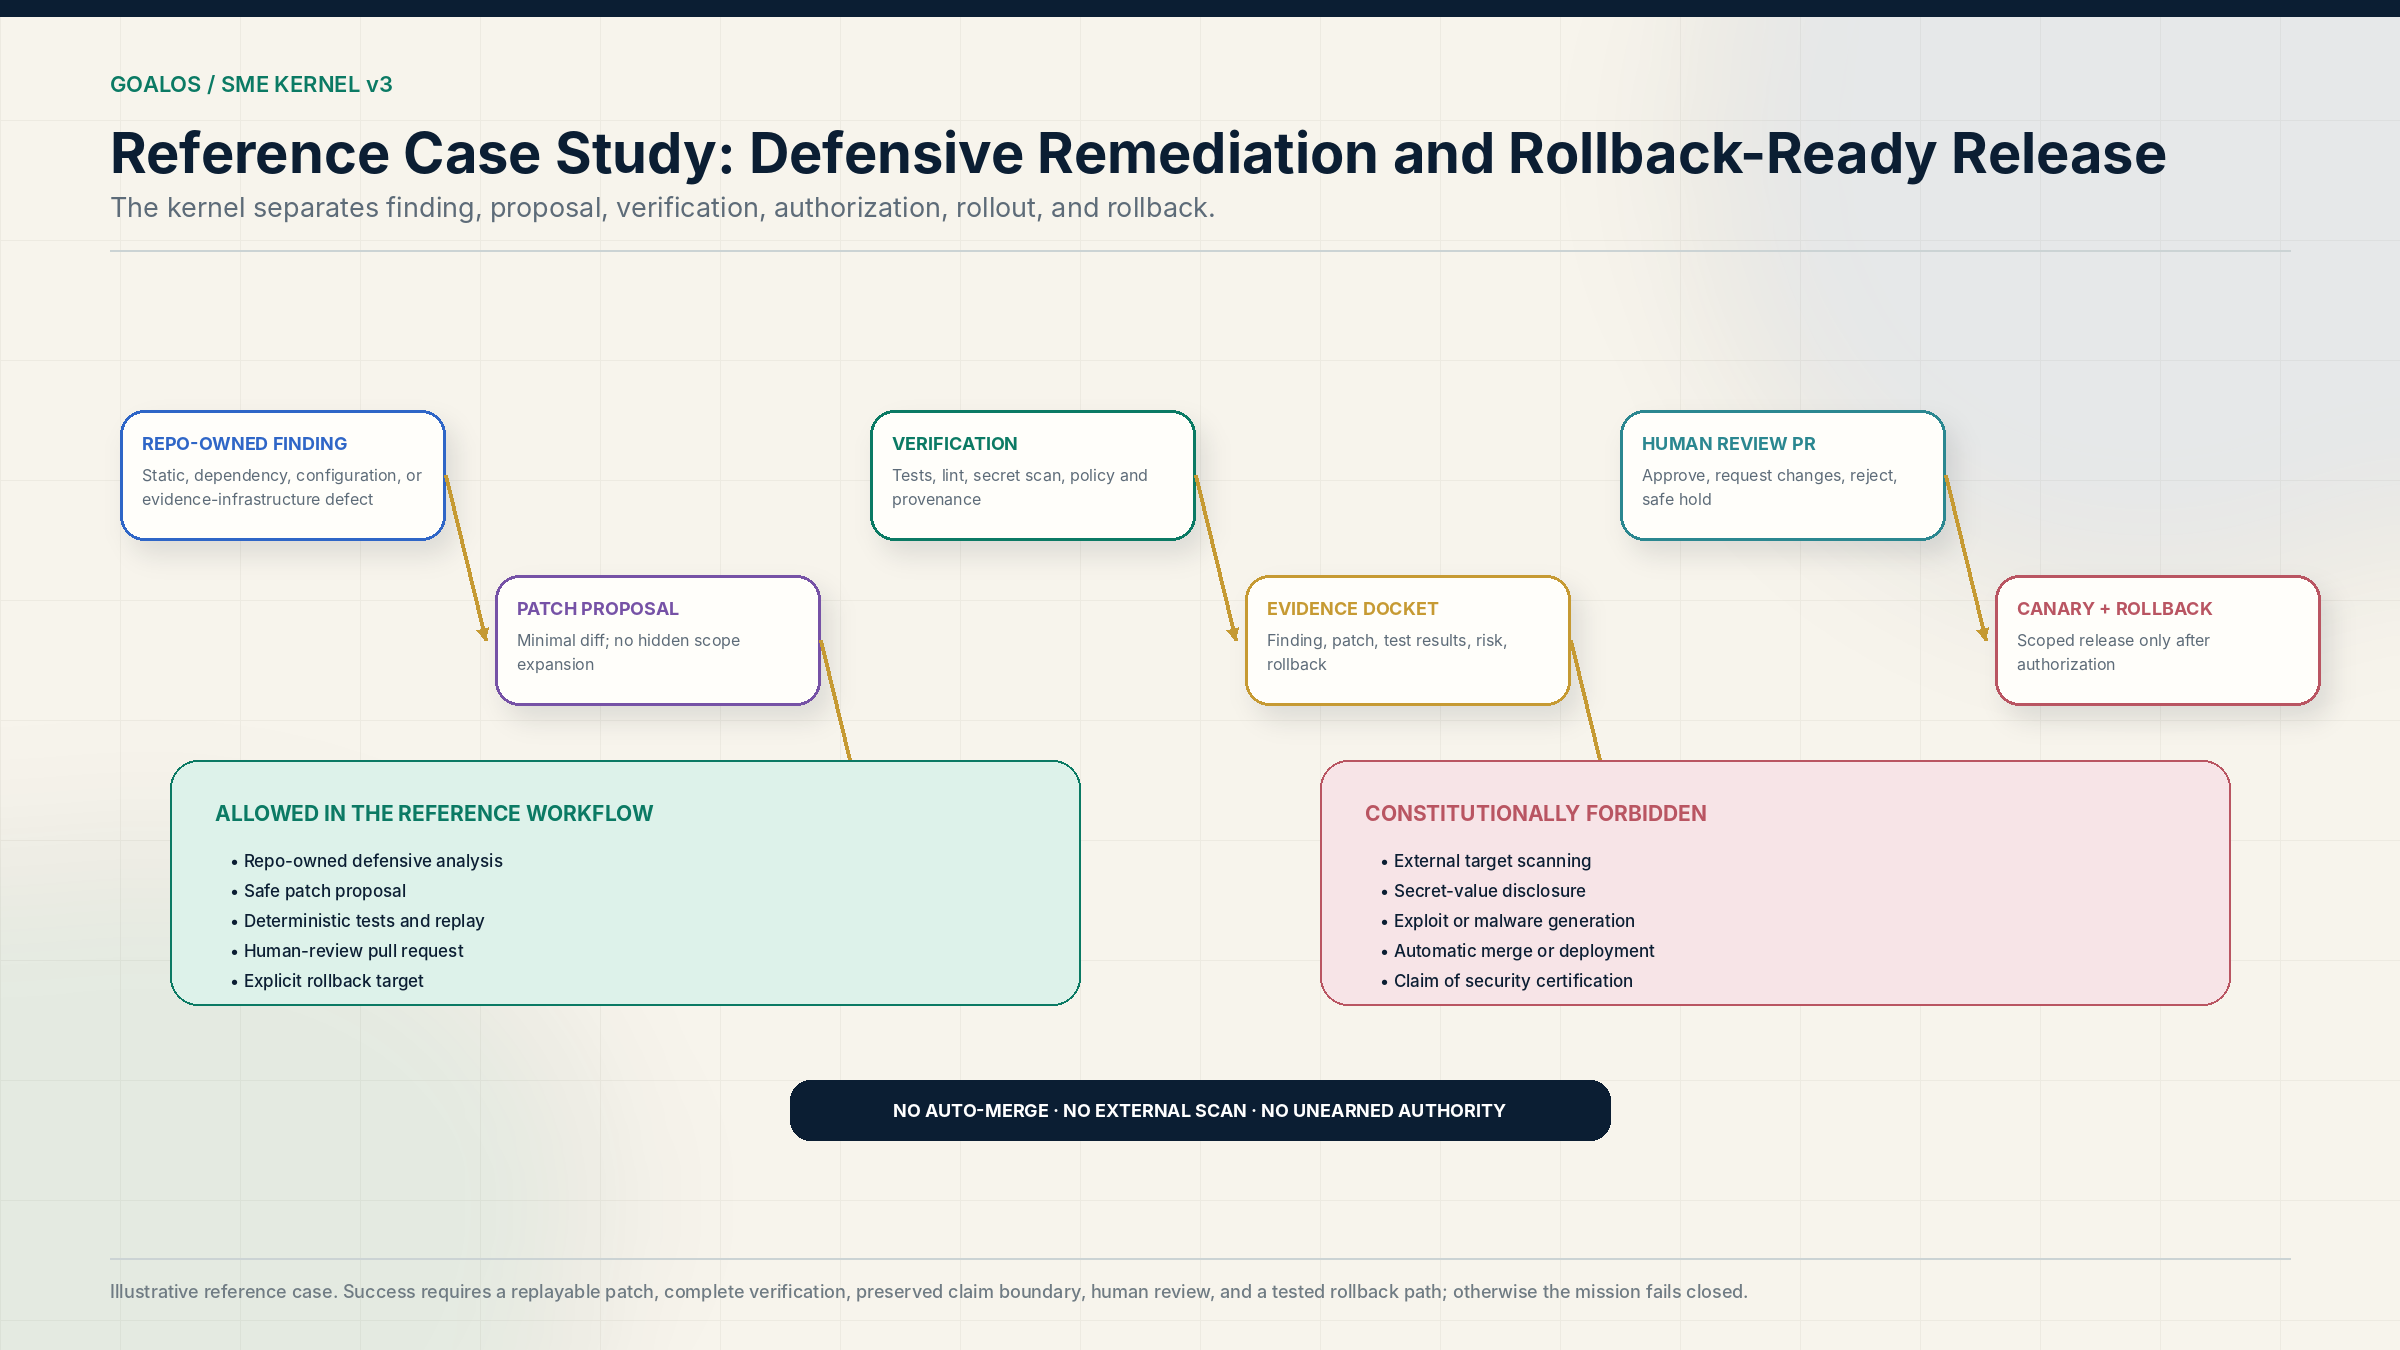
\includegraphics[width=6.75in,height=3.79687in]{media/image19.png}

Figure 19. Reference Case Study C: defensive remediation and
rollback-ready release. Finding, patch, verification, authorization,
rollout, and rollback remain distinct stages with distinct authorities.

\begin{longtable}[]{@{}
  >{\raggedright\arraybackslash}p{(\columnwidth - 2\tabcolsep) * \real{0.5000}}
  >{\raggedright\arraybackslash}p{(\columnwidth - 2\tabcolsep) * \real{0.5000}}@{}}
\toprule\noalign{}
\begin{minipage}[b]{\linewidth}\raggedright
\textbf{Docket component}
\end{minipage} & \begin{minipage}[b]{\linewidth}\raggedright
\textbf{Required record}
\end{minipage} \\
\midrule\noalign{}
\endhead
\bottomrule\noalign{}
\endlastfoot
\textbf{Finding proof} & Exact repository location, affected behavior,
source of the finding, reproducibility, confidence, and false-positive
analysis. \\
\textbf{Patch contract} & Minimal scope, intended effect, prohibited
side effects, dependency changes, and rollback target. \\
\textbf{Verification} & Unit/integration tests, static analysis,
secret-token scan, policy checks, change-scope diff, and deterministic
replay. \\
\textbf{Human review} & A pull request carries the Evidence Docket. A
human may approve, request changes, reject, or place the mission in safe
hold. \\
\textbf{Release control} & Production release remains a separate
authorization. Canary scope, monitoring, safety thresholds, and rollback
are required before propagation. \\
\textbf{Hard invariants} & Raw secret leakage=0; external target
scans=0; exploit execution=0; malware generation=0; unsafe
auto-merge=0. \\
\textbf{Falsification} & The case fails if the finding cannot be
replayed, the patch expands scope silently, tests are missing, secret
material appears, or rollback is undefined. \\
\end{longtable}

\subsection{21.4 Case Study D - cold-chain energy resilience and
capability
compounding}\label{case-study-d---cold-chain-energy-resilience-and-capability-compounding}

Mission. An operator wants to reduce cold-chain energy waste and failure
risk without compromising product integrity. The reference mission
constructs a baseline, generates bounded interventions, tests them in a
proxy or simulation, compares treatment and control, and produces a
measurement-ready pilot plan.

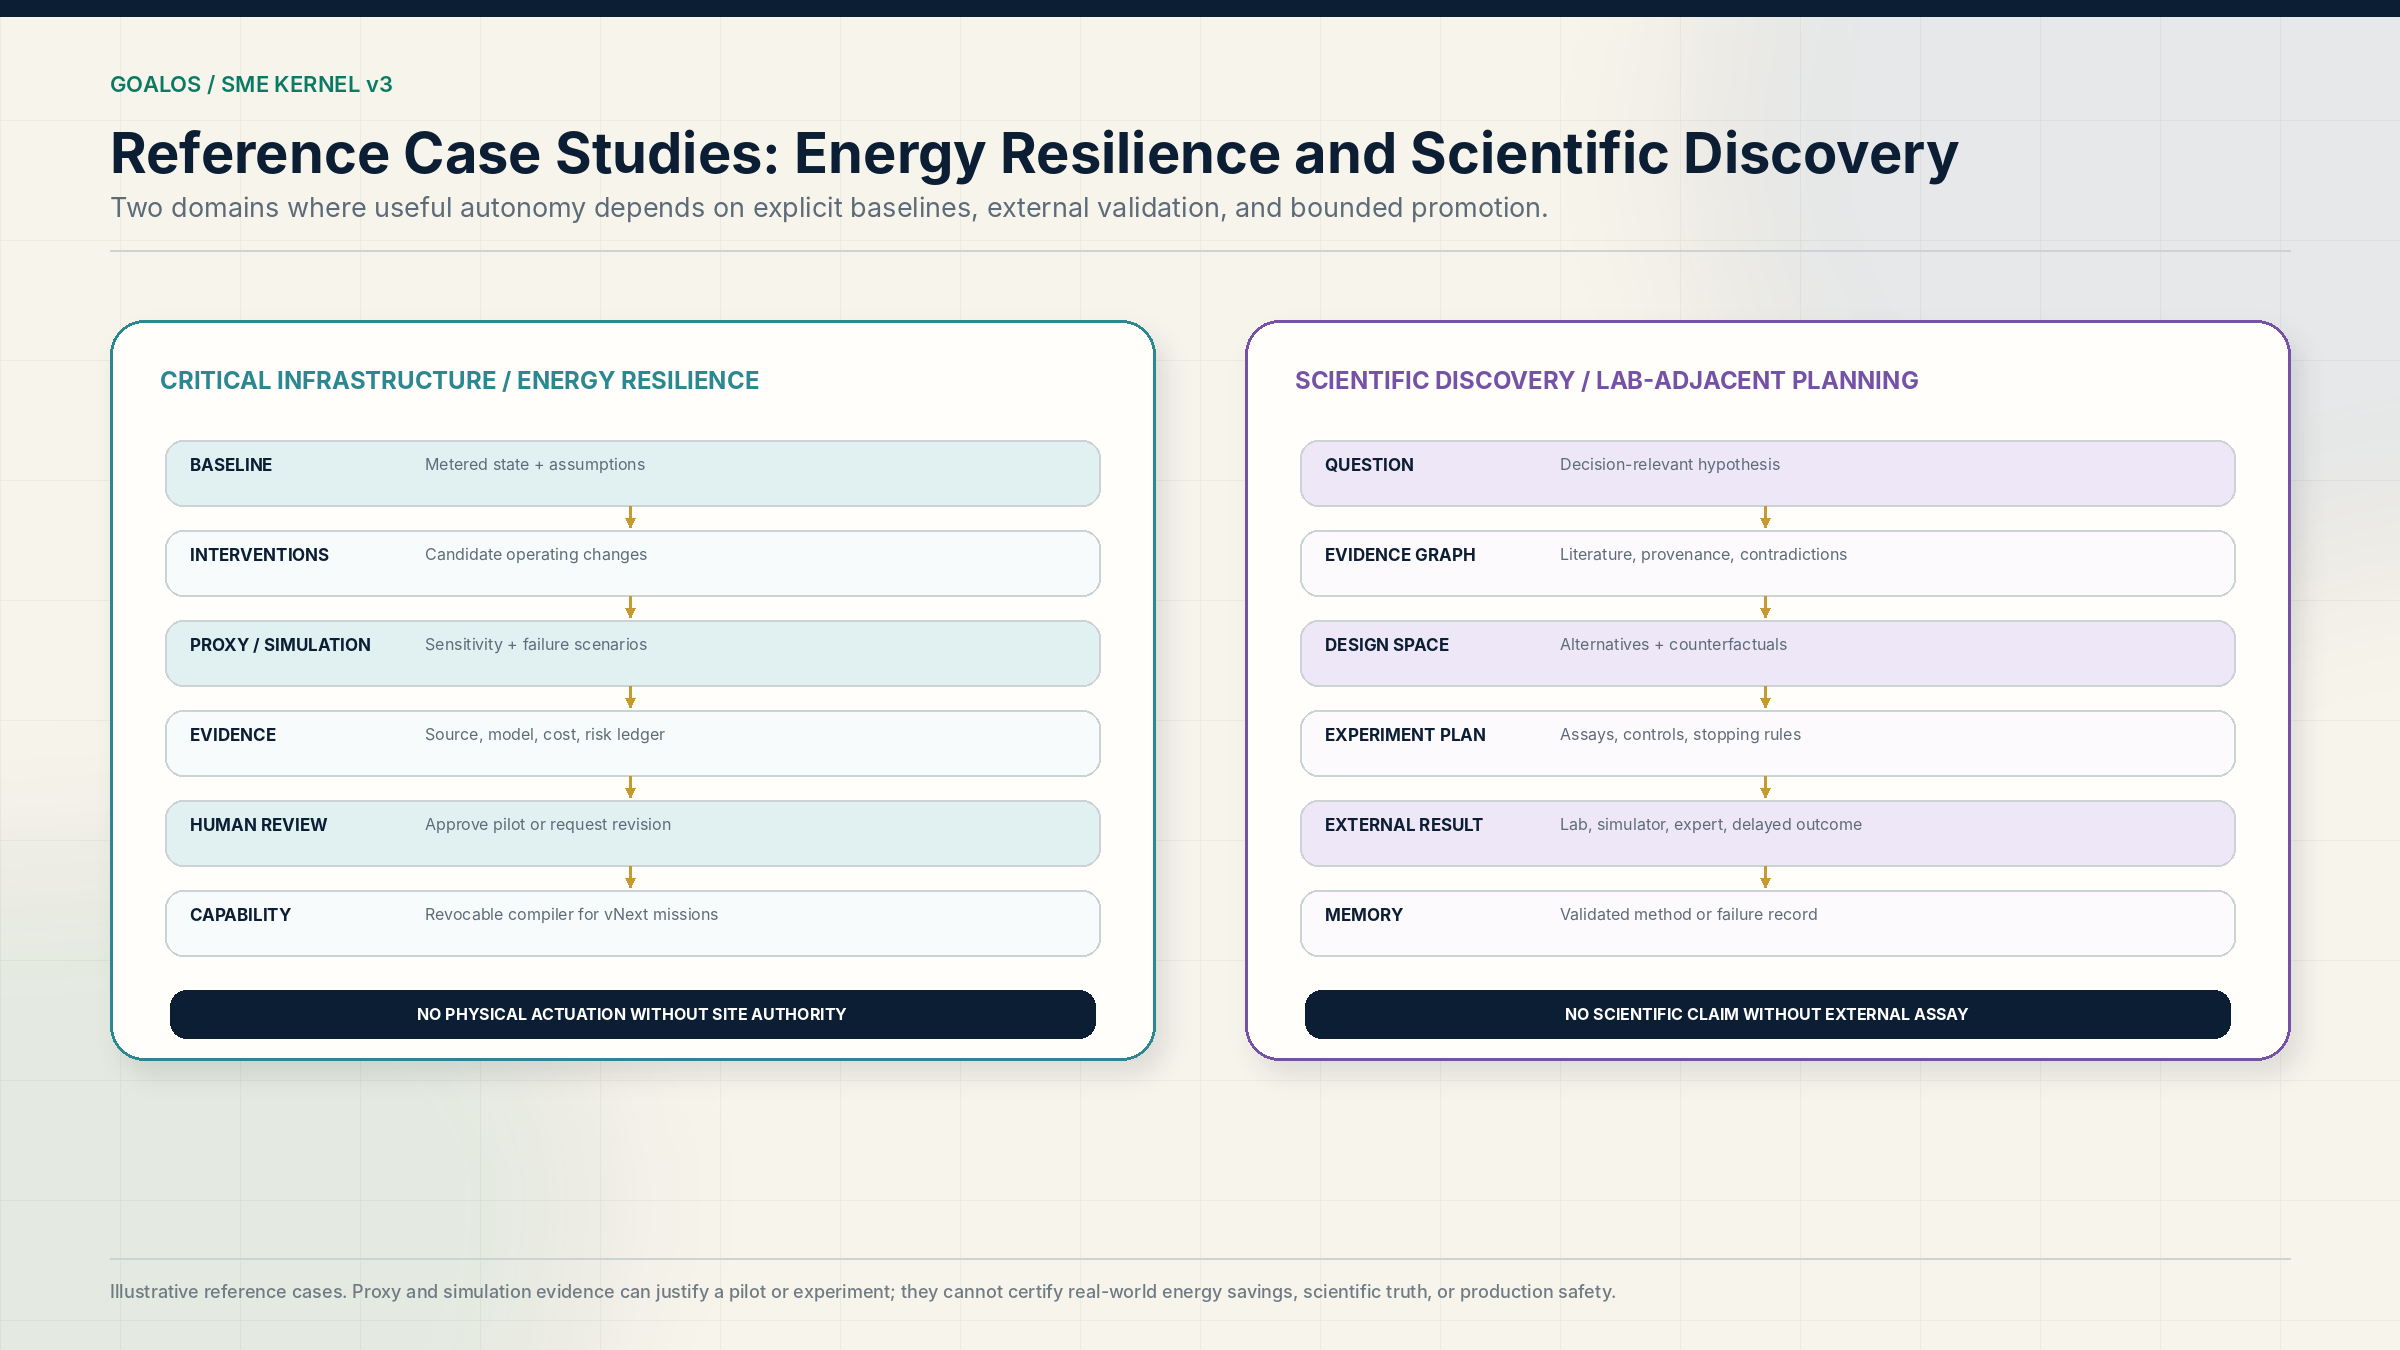
\includegraphics[width=6.75in,height=3.79687in]{media/image20.png}

Figure 20. Reference Case Studies D and E. Energy resilience and
scientific discovery use the same constitutional pattern, but each
requires domain-specific external authority before a proxy result can
become a real-world claim.

\begin{longtable}[]{@{}
  >{\raggedright\arraybackslash}p{(\columnwidth - 2\tabcolsep) * \real{0.5000}}
  >{\raggedright\arraybackslash}p{(\columnwidth - 2\tabcolsep) * \real{0.5000}}@{}}
\toprule\noalign{}
\begin{minipage}[b]{\linewidth}\raggedright
\textbf{Case element}
\end{minipage} & \begin{minipage}[b]{\linewidth}\raggedright
\textbf{Energy-resilience reference}
\end{minipage} \\
\midrule\noalign{}
\endhead
\bottomrule\noalign{}
\endlastfoot
\textbf{Baseline} & Energy, temperature, throughput, failure,
maintenance, and operating-state assumptions are versioned and
challengeable. \\
\textbf{Intervention set} & Scheduling, setpoint, defrost, load
balancing, maintenance, and control alternatives are proposed with
safety constraints. \\
\textbf{Evidence contact} & Simulation or historical backtest remains
proxy evidence. A real pilot requires site authorization,
instrumentation, and a predeclared measurement plan. \\
\textbf{Decision state} & The operator receives ranked interventions,
sensitivity analysis, safety and cost ledger, pilot design, stop
conditions, and rollback. \\
\textbf{Capability package} & A successful pilot may produce a revocable
resilience compiler: the reusable method, not an unconditional control
policy. \\
\textbf{Metrics} & Energy per unit throughput, temperature excursions,
spoilage proxy, maintenance burden, recovery time, cost, and
evidence-transfer performance. \\
\textbf{Falsification} & The case fails if baseline drift explains the
apparent gain, safety worsens, instrumentation is inadequate, or
improvements do not survive delayed outcome checks. \\
\end{longtable}

Claim boundary. The reference case may demonstrate a proof-producing
workflow and a pilot-ready decision package. It does not establish
real-world energy savings, safety certification, or infrastructure
performance without site evidence.

\subsection{21.5 Case Study E - scientific discovery and experimental
design}\label{case-study-e---scientific-discovery-and-experimental-design}

Mission. A research program must choose which hypotheses deserve scarce
experimental capacity. Kernel v3 maps sources and contradictions,
generates competing mechanisms, designs controls, estimates information
value, and prepares an experiment sequence. The decisive evidence comes
from external assays, simulations with validated fidelity, expert
review, or delayed outcomes - not from the persuasiveness of the
hypothesis text.

\begin{longtable}[]{@{}
  >{\raggedright\arraybackslash}p{(\columnwidth - 2\tabcolsep) * \real{0.5000}}
  >{\raggedright\arraybackslash}p{(\columnwidth - 2\tabcolsep) * \real{0.5000}}@{}}
\toprule\noalign{}
\begin{minipage}[b]{\linewidth}\raggedright
\textbf{Scientific object}
\end{minipage} & \begin{minipage}[b]{\linewidth}\raggedright
\textbf{Kernel output}
\end{minipage} \\
\midrule\noalign{}
\endhead
\bottomrule\noalign{}
\endlastfoot
\textbf{Question contract} & Scientific question, decision to support,
known constraints, excluded domains, success and falsification
criteria. \\
\textbf{Evidence graph} & Primary papers, datasets, provenance,
freshness, methodological quality, conflicting findings, and unresolved
assumptions. \\
\textbf{Design space} & Hypotheses, mechanisms, counterfactuals,
expected observations, failure modes, and alternative explanations. \\
\textbf{Experiment plan} & Controls, randomization where applicable,
measurement, safety, sample-size rationale, stop rules, and analysis
plan. \\
\textbf{Validation} & External assay, benchmark, simulation with known
validity, or independent expert review; status remains explicit. \\
\textbf{Memory} & Validated methods and failed hypotheses are stored
with lineage so future missions inherit evidence rather than
folklore. \\
\textbf{Falsification} & The case fails if the proposal lacks
discriminating tests, confounds are ignored, evidence provenance is
weak, or negative results are omitted. \\
\end{longtable}

\subsection{21.6 Case Study F - public policy option
mission}\label{case-study-f---public-policy-option-mission}

Mission. A public or institutional body must compare policy options
under uncertain evidence, competing values, legal constraints, and
distributional effects. The kernel structures the work without claiming
legal authority: primary sources are dated, stakeholder claims remain
attributed, conflicts are preserved, and each option is linked to
assumptions, implementation dependencies, monitoring, and reversal
conditions.

\begin{longtable}[]{@{}
  >{\raggedright\arraybackslash}p{(\columnwidth - 2\tabcolsep) * \real{0.5000}}
  >{\raggedright\arraybackslash}p{(\columnwidth - 2\tabcolsep) * \real{0.5000}}@{}}
\toprule\noalign{}
\begin{minipage}[b]{\linewidth}\raggedright
\textbf{Control}
\end{minipage} & \begin{minipage}[b]{\linewidth}\raggedright
\textbf{Public-policy reference case}
\end{minipage} \\
\midrule\noalign{}
\endhead
\bottomrule\noalign{}
\endlastfoot
\textbf{Evidence integrity} & Primary law and official guidance are
separated from commentary, advocacy, and model inference. \\
\textbf{Plurality} & At least one independent dissent path must survive
into the decision package; consensus is not manufactured by
summarization. \\
\textbf{Impact model} & Benefits, costs, distributional effects,
implementation burden, uncertainty, and second-order risks are
scenario-based and source-bound. \\
\textbf{Authority} & The output supports deliberation only. Legal
interpretation, enactment, enforcement, funding, and public
communication remain authorized institutional acts. \\
\textbf{Metrics} & Source freshness, stakeholder coverage, contradiction
coverage, assumption sensitivity, distributional visibility, and
reviewer traceability. \\
\textbf{Falsification} & The case fails if legal sources are outdated,
affected groups are absent, uncertainty is hidden, or a single objective
function erases legitimate value conflict. \\
\end{longtable}

\subsection{21.7 Case Study G - proof-gated agentic work
market}\label{case-study-g---proof-gated-agentic-work-market}

Mission. A sponsor commissions a bounded machine-labor job. Multiple
institutions commit bids; a coalition is selected; an Alpha Node
executes; a proof parliament evaluates; a dissent memorandum is
preserved; a challenge window resolves disputes; and a settlement intent
is prepared for human review.

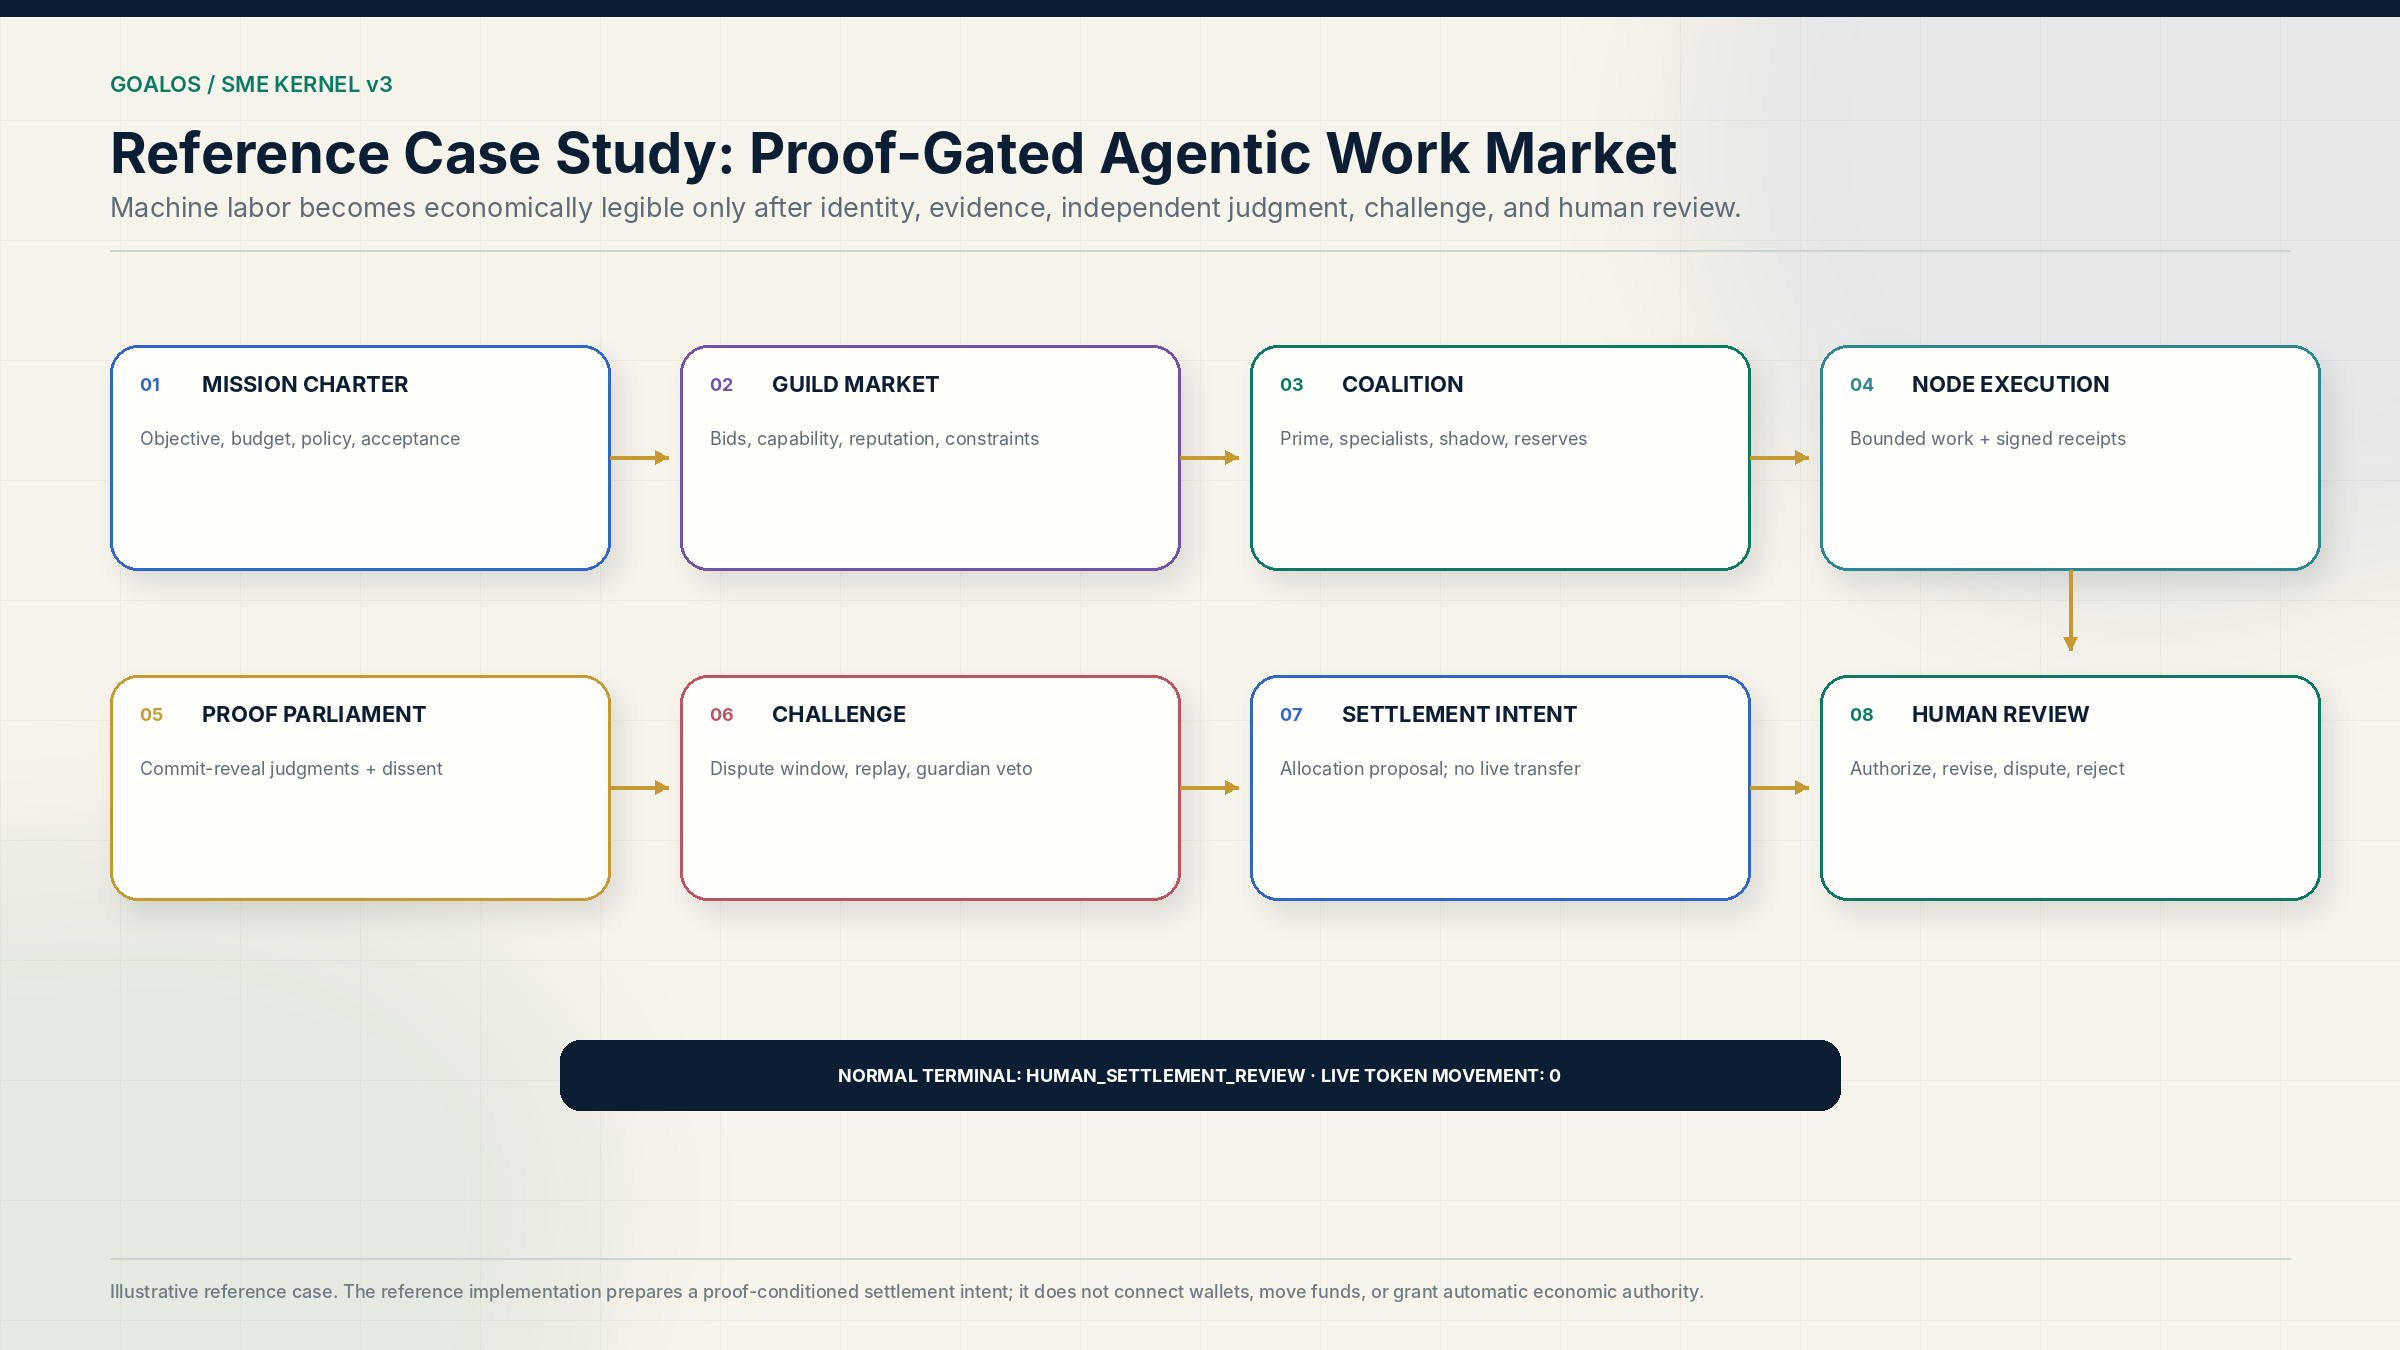
\includegraphics[width=6.75in,height=3.79687in]{media/image21.png}

Figure 21. Reference Case Study G: proof-gated agentic work market.
Economic coordination follows evidence and challenge; the reference
system prepares settlement intent but moves no live value.

\begin{longtable}[]{@{}
  >{\raggedright\arraybackslash}p{(\columnwidth - 2\tabcolsep) * \real{0.5000}}
  >{\raggedright\arraybackslash}p{(\columnwidth - 2\tabcolsep) * \real{0.5000}}@{}}
\toprule\noalign{}
\begin{minipage}[b]{\linewidth}\raggedright
\textbf{Institutional mechanism}
\end{minipage} & \begin{minipage}[b]{\linewidth}\raggedright
\textbf{Reference requirement}
\end{minipage} \\
\midrule\noalign{}
\endhead
\bottomrule\noalign{}
\endlastfoot
\textbf{Identity and admission} & Every institution, node, validator,
and authority has a declared role, scope, and evidence history. \\
\textbf{Market design} & Bids are compared across capability, evidence,
reliability, cost, safety, energy, and policy fit rather than a single
price. \\
\textbf{Coalition structure} & Prime, specialists, shadow institution,
and reserves create execution capacity and adversarial review. \\
\textbf{Execution proof} & The node emits bounded work receipts,
resource records, artifacts, and predecessor-linked commitments. \\
\textbf{Proof parliament} & Independent seats commit and reveal
judgments. Dissent is preserved; guardian vetoes and challenge rights
remain active. \\
\textbf{Settlement posture} & The system calculates a transparent
contribution and allocation proposal, but the reference implementation
does not connect wallets or transfer tokens. \\
\textbf{Success metrics} & Proof completeness, replay rate, validator
independence, false acceptance, dispute resolution, contribution
fidelity, latency, and human-review burden. \\
\textbf{Falsification} & The case fails if validators herd, evidence
cannot be replayed, contribution is opaque, challenge is ineffective, or
settlement can occur without authority. \\
\end{longtable}

\subsection{21.8 Portfolio metrics and adoption
discipline}\label{portfolio-metrics-and-adoption-discipline}

Across use cases, the kernel should be evaluated by a common portfolio
of measures rather than domain-specific success alone. These metrics
prevent local wins from hiding institutional failure.

\begin{longtable}[]{@{}
  >{\raggedright\arraybackslash}p{(\columnwidth - 2\tabcolsep) * \real{0.5000}}
  >{\raggedright\arraybackslash}p{(\columnwidth - 2\tabcolsep) * \real{0.5000}}@{}}
\toprule\noalign{}
\begin{minipage}[b]{\linewidth}\raggedright
\textbf{Metric family}
\end{minipage} & \begin{minipage}[b]{\linewidth}\raggedright
\textbf{Cross-case measurement}
\end{minipage} \\
\midrule\noalign{}
\endhead
\bottomrule\noalign{}
\endlastfoot
\textbf{Proof integrity} & Share of material claims with evidence or
explicit uncertainty; signature and commitment validity; provenance
completeness. \\
\textbf{Permission quality} & False permission, false denial, escalation
quality, and whether the scope of human certificates matches the
evidence. \\
\textbf{Replay and challenge} & Independent replay success, dispute
resolution, dissent preservation, and tamper rejection. \\
\textbf{Decision effectiveness} & Time to review-ready state, reviewer
comprehension, option clarity, action-condition completeness, and
delayed outcome. \\
\textbf{Safety and governance} & Blocked forbidden actions, privilege
violations, secret leakage, rollback readiness, incident rate, and
authority separation. \\
\textbf{Economic efficiency} & Verified value per cost, review burden,
coordination overhead, validation cost, settlement latency, and reuse
lift. \\
\textbf{Compounding} & Capability-package reuse, transfer to adjacent
missions, failure-memory use, expiry discipline, and regression rate. \\
\end{longtable}

\begin{longtable}[]{@{}
  >{\raggedright\arraybackslash}p{(\columnwidth - 0\tabcolsep) * \real{1.0000}}@{}}
\toprule\noalign{}
\begin{minipage}[b]{\linewidth}\raggedright
\textbf{Adoption law.} Start with one narrow, evidence-rich workflow.
Earn the right to expand only after replay, human review, delayed
outcomes, and rollback prove that the institution is becoming more
reliable - not merely more autonomous.
\end{minipage} \\
\midrule\noalign{}
\endhead
\bottomrule\noalign{}
\endlastfoot
\end{longtable}

\section{22. Conformance and
interoperability}\label{conformance-and-interoperability}

Kernel v3 can be adopted incrementally. Conformance is defined by
behavior and evidence, not branding.

\begin{longtable}[]{@{}
  >{\raggedright\arraybackslash}p{(\columnwidth - 4\tabcolsep) * \real{0.3333}}
  >{\raggedright\arraybackslash}p{(\columnwidth - 4\tabcolsep) * \real{0.3333}}
  >{\raggedright\arraybackslash}p{(\columnwidth - 4\tabcolsep) * \real{0.3333}}@{}}
\toprule\noalign{}
\begin{minipage}[b]{\linewidth}\raggedright
\textbf{Level}
\end{minipage} & \begin{minipage}[b]{\linewidth}\raggedright
\textbf{Name}
\end{minipage} & \begin{minipage}[b]{\linewidth}\raggedright
\textbf{Requirement}
\end{minipage} \\
\midrule\noalign{}
\endhead
\bottomrule\noalign{}
\endlastfoot
\textbf{L0} & Documented & Mission, roles, states, envelopes, claim
boundary, and threat model are declared. \\
\textbf{L1} & Schema-valid & Objects and bundles validate against
versioned schemas; canonicalization rules are declared. \\
\textbf{L2} & State-enforced & Illegal state transitions and issuers are
rejected by an interface-independent kernel. \\
\textbf{L3} & Signed and replayable & Every accepted event is linked,
signed, persisted, exportable, and strictly replayable. \\
\textbf{L4} & Independently attestable & External evaluators can verify
bundles, sign opinions, preserve dissent, and challenge. \\
\textbf{L5} & Human-gated production & Consequential actions require
scoped certificates, expiry, revocation, monitoring, and rollback. \\
\textbf{L6} & Cross-institutional & Proof-carrying artifacts and
certificates interoperate without exposing private intelligence. \\
\end{longtable}

\subsection{22.1 Normative vocabulary}\label{normative-vocabulary}

MUST denotes a requirement for conformance. MUST NOT denotes a
prohibited behavior. SHOULD denotes a recommendation that may be
departed from only with documented institutional justification. MAY
denotes an optional feature. PUBLIC denotes information safe for proof
publication under declared policy. PRIVATE denotes information retained
in controlled storage and exposed only through scoped audit.

\subsection{22.2 Versioning and
compatibility}\label{versioning-and-compatibility}

Every envelope and bundle must identify protocol and schema versions.
Verifiers must reject unknown mandatory fields or unsupported major
versions, and must not silently downgrade cryptographic, authority, or
evidence requirements. Migration should produce a new signed event or
bundle, not rewrite the old record.

\subsection{22.3 Standards alignment without false
conformance}\label{standards-alignment-without-false-conformance}

The architecture is informed by RFC 8032, WebCrypto, IndexedDB, Web
Workers, JSON canonicalization, verifiable credentials, NIST AI RMF,
proof-carrying code, and GitHub Pages custom workflows {[}5-14{]}. The
reference release does not claim full conformance to standards unless
explicitly tested. Alignment is a roadmap, not a label.

\section{23. Limitations, falsification, and claim
boundaries}\label{limitations-falsification-and-claim-boundaries}

\subsection{23.1 Limitations}\label{limitations}

\begin{itemize}
\item
  The reference adapters are deterministic local fixtures and do not
  demonstrate live model reasoning, external tool use, or real
  enterprise workflows.
\item
  Local Ed25519 signatures do not establish legal identity,
  organizational independence, key custody quality, or factual
  correctness.
\item
  IndexedDB persistence is local browser storage, not a distributed
  availability guarantee or immutable institutional ledger.
\item
  The current independent verifier runs client-side and is not an
  independent organization.
\item
  The Evidence Docket structure can organize weak evidence as well as
  strong evidence; evidence quality still depends on sources, methods,
  and evaluators.
\item
  The architecture adds governance cost and may be unnecessary for
  low-consequence work.
\item
  Human review can be slow, inconsistent, captured, or perfunctory;
  human involvement is not a magic safety guarantee.
\item
  No production claims can be made until real adapters, real tasks,
  strong baselines, external validation, delayed outcomes, and incident
  records exist.
\end{itemize}

\subsection{23.2 Falsification
conditions}\label{falsification-conditions}

\begin{longtable}[]{@{}
  >{\raggedright\arraybackslash}p{(\columnwidth - 2\tabcolsep) * \real{0.5000}}
  >{\raggedright\arraybackslash}p{(\columnwidth - 2\tabcolsep) * \real{0.5000}}@{}}
\toprule\noalign{}
\begin{minipage}[b]{\linewidth}\raggedright
\textbf{Condition}
\end{minipage} & \begin{minipage}[b]{\linewidth}\raggedright
\textbf{The thesis is weakened or rejected if...}
\end{minipage} \\
\midrule\noalign{}
\endhead
\bottomrule\noalign{}
\endlastfoot
\textbf{Proof is not predictive} & Evidence-complete candidates do not
outperform or remain safer than strong baselines on held-out tasks. \\
\textbf{Baselines win} & Single-agent or fixed-workflow systems produce
equal or better verified work at lower total cost and risk. \\
\textbf{Gate is gameable} & Adapters or evaluators learn to satisfy
protocol metrics while degrading real outcomes. \\
\textbf{Authority boundary fails} & Machine-complete work can trigger
external consequence without a valid scoped human certificate. \\
\textbf{Replay is unreliable} & Equivalent valid bundles produce
inconsistent results, or tampered bundles are accepted. \\
\textbf{Privacy boundary breaks} & Public proof leaks private prompts,
customer data, secrets, or privileged rationale. \\
\textbf{Rollback fails} & Approved capability cannot be scoped, revoked,
or reverted when conditions change. \\
\textbf{Governance overhead dominates} & Verification and review cost
exceeds the avoided proof debt and delivered verified value. \\
\textbf{Reuse does not compound} & Capability packages do not improve
later held-out missions or reduce cost/risk. \\
\end{longtable}

\subsection{23.3 Claim boundary}\label{claim-boundary}

\begin{longtable}[]{@{}
  >{\raggedright\arraybackslash}p{(\columnwidth - 0\tabcolsep) * \real{1.0000}}@{}}
\toprule\noalign{}
\begin{minipage}[b]{\linewidth}\raggedright
\textbf{Publication-safe claim.}

GoalOS AGIALPHA Ascension Sovereign Machine Economy Kernel v3 is a
proof-to-permission architecture, executable browser-local reference
implementation, and falsifiable evaluation program. It does not claim
achieved AGI or ASI, empirical SOTA, legal identity, independent
certification, guaranteed ROI, production authorization, live
settlement, user-fund authorization, autonomous sovereignty, energy
abundance, or civilization-scale capability.
\end{minipage} \\
\midrule\noalign{}
\endhead
\bottomrule\noalign{}
\endlastfoot
\end{longtable}

\section{24. Conclusion: the constitutional operating system for
autonomous
work}\label{conclusion-the-constitutional-operating-system-for-autonomous-work}

The central problem of institutional AI is not whether a model can
generate an answer or whether an agent can call a tool. It is whether an
organization can know what was asked, what was done, what evidence
exists, who evaluated it, what remains uncertain, what rights can be
challenged, which actions are reversible, and who is authorized to
create consequence.

GoalOS Mission OS supplies the objective-to-decision product layer. AGI
ALPHA supplies the organizational substrate. AEP-001 supplies the law of
proof-backed evolution. The Sovereign Machine Economy integrates
institution formation, node execution, work markets, validation,
challenge, settlement intent, and memory. Kernel v3 supplies the
executable constitution beneath them.

Minds may form. Nodes may execute. Markets may coordinate. Proof may
accumulate. Humans authorize consequence.

The paper's strongest claim is deliberately narrow: a
proof-to-permission kernel can make autonomous work more inspectable,
challengeable, replayable, and revocable than output-only or agent-only
systems. The next proof is not another statement of ambition. It is an
independently reproduced, paid, real-task mission portfolio in which
authenticated evidence, strong baselines, separated validators, human
review, rollback, and delayed outcomes show that the architecture
produces more verified work per unit cost and risk.

\begin{longtable}[]{@{}
  >{\raggedright\arraybackslash}p{(\columnwidth - 0\tabcolsep) * \real{1.0000}}@{}}
\toprule\noalign{}
\begin{minipage}[b]{\linewidth}\raggedright
\textbf{One-page constitution.}

Identify. Out-Learn. Out-Think. Out-Design. Out-Strategise. Out-Execute.
Aim. Act. Prove. Evolve. AI creates output. GoalOS creates proof. A
model can answer. An agent can act. An institution must prove. No proof,
no evolution. No eval, no propagation. No rollback, no release. Replace
the intelligence, never the constitution.
\end{minipage} \\
\midrule\noalign{}
\endhead
\bottomrule\noalign{}
\endlastfoot
\end{longtable}

\section{Appendix A. State transition
registry}\label{appendix-a.-state-transition-registry}

\begin{longtable}[]{@{}
  >{\raggedright\arraybackslash}p{(\columnwidth - 8\tabcolsep) * \real{0.2000}}
  >{\raggedright\arraybackslash}p{(\columnwidth - 8\tabcolsep) * \real{0.2000}}
  >{\raggedright\arraybackslash}p{(\columnwidth - 8\tabcolsep) * \real{0.2000}}
  >{\raggedright\arraybackslash}p{(\columnwidth - 8\tabcolsep) * \real{0.2000}}
  >{\raggedright\arraybackslash}p{(\columnwidth - 8\tabcolsep) * \real{0.2000}}@{}}
\toprule\noalign{}
\begin{minipage}[b]{\linewidth}\raggedright
\textbf{\#}
\end{minipage} & \begin{minipage}[b]{\linewidth}\raggedright
\textbf{State}
\end{minipage} & \begin{minipage}[b]{\linewidth}\raggedright
\textbf{Plane}
\end{minipage} & \begin{minipage}[b]{\linewidth}\raggedright
\textbf{Issuer}
\end{minipage} & \begin{minipage}[b]{\linewidth}\raggedright
\textbf{Predecessor}
\end{minipage} \\
\midrule\noalign{}
\endhead
\bottomrule\noalign{}
\endlastfoot
\textbf{1} & DRAFT & KERNEL & SYSTEM & START \\
\textbf{2} & MISSION\_\allowbreak{}COMMITTED & KERNEL & HUMAN\_\allowbreak{}REVIEWER & DRAFT \\
\textbf{3} & INSTITUTION\_\allowbreak{}PROPOSED & MIND & META\_\allowbreak{}ARCHITECT &
MISSION\_\allowbreak{}COMMITTED \\
\textbf{4} & INSTITUTION\_\allowbreak{}CHARTERED & MIND & META\_\allowbreak{}ARCHITECT &
INSTITUTION\_\allowbreak{}PROPOSED \\
\textbf{5} & NODE\_\allowbreak{}ADMITTED & NODE & NODE\_\allowbreak{}OPERATOR &
INSTITUTION\_\allowbreak{}CHARTERED \\
\textbf{6} & EXECUTION\_\allowbreak{}BOUNDED & NODE & NODE\_\allowbreak{}OPERATOR &
NODE\_\allowbreak{}ADMITTED \\
\textbf{7} & WORK\_\allowbreak{}EXECUTED & NODE & NODE\_\allowbreak{}OPERATOR &
EXECUTION\_\allowbreak{}BOUNDED \\
\textbf{8} & EVIDENCE\_\allowbreak{}SEALED & PROOF & NODE\_\allowbreak{}OPERATOR &
WORK\_\allowbreak{}EXECUTED \\
\textbf{9} & MARKET\_\allowbreak{}CONVENED & MARKET & MARKET\_\allowbreak{}STEWARD &
EVIDENCE\_\allowbreak{}SEALED \\
\textbf{10} & VALIDATION\_\allowbreak{}COMMITTED & PROOF & INDEPENDENT\_\allowbreak{}VERIFIER &
MARKET\_\allowbreak{}CONVENED \\
\textbf{11} & VALIDATION\_\allowbreak{}REVEALED & PROOF & INDEPENDENT\_\allowbreak{}VERIFIER &
VALIDATION\_\allowbreak{}COMMITTED \\
\textbf{12} & CHALLENGE\_\allowbreak{}WINDOW\_\allowbreak{}OPEN & RIGHTS & INDEPENDENT\_\allowbreak{}VERIFIER &
VALIDATION\_\allowbreak{}REVEALED \\
\textbf{13} & SETTLEMENT\_\allowbreak{}INTENT\_\allowbreak{}PREPARED & MARKET & MARKET\_\allowbreak{}STEWARD &
CHALLENGE\_\allowbreak{}WINDOW\_\allowbreak{}OPEN \\
\textbf{14} & AWAITING\_\allowbreak{}HUMAN\_\allowbreak{}REVIEW & HUMAN & INDEPENDENT\_\allowbreak{}VERIFIER &
SETTLEMENT\_\allowbreak{}INTENT\_\allowbreak{}PREPARED \\
\textbf{15} & HUMAN\_\allowbreak{}REVIEW\_\allowbreak{}RECORDED & HUMAN & HUMAN\_\allowbreak{}REVIEWER &
AWAITING\_\allowbreak{}HUMAN\_\allowbreak{}REVIEW \\
\textbf{16} & MEMORY\_\allowbreak{}DISPOSITION\_\allowbreak{}RECORDED & MEMORY & HUMAN\_\allowbreak{}REVIEWER &
HUMAN\_\allowbreak{}REVIEW\_\allowbreak{}RECORDED \\
\textbf{17} & COMPLETE & KERNEL & HUMAN\_\allowbreak{}REVIEWER &
MEMORY\_\allowbreak{}DISPOSITION\_\allowbreak{}RECORDED \\
\end{longtable}

\section{Appendix B. Envelope registry and minimum
fields}\label{appendix-b.-envelope-registry-and-minimum-fields}

\begin{longtable}[]{@{}
  >{\raggedright\arraybackslash}p{(\columnwidth - 4\tabcolsep) * \real{0.3333}}
  >{\raggedright\arraybackslash}p{(\columnwidth - 4\tabcolsep) * \real{0.3333}}
  >{\raggedright\arraybackslash}p{(\columnwidth - 4\tabcolsep) * \real{0.3333}}@{}}
\toprule\noalign{}
\begin{minipage}[b]{\linewidth}\raggedright
\textbf{Envelope}
\end{minipage} & \begin{minipage}[b]{\linewidth}\raggedright
\textbf{Issuer}
\end{minipage} & \begin{minipage}[b]{\linewidth}\raggedright
\textbf{Minimum payload expectation}
\end{minipage} \\
\midrule\noalign{}
\endhead
\bottomrule\noalign{}
\endlastfoot
\textbf{MissionCommitment} & HUMAN\_\allowbreak{}REVIEWER & Binds mission,
constraints, risk, deliverables, and prohibited actions. \\
\textbf{InstitutionProposal} & META\_\allowbreak{}ARCHITECT & Proposes a bounded
multi-agent institution and alternatives. \\
\textbf{InstitutionCharter} & META\_\allowbreak{}ARCHITECT & Seals roles, policies,
stop conditions, and authority limits. \\
\textbf{NodeAdmission} & NODE\_\allowbreak{}OPERATOR & Binds node identity,
resources, primary route, and shadow route. \\
\textbf{NodeExecutionReceipt} & NODE\_\allowbreak{}OPERATOR & Records bounded
execution trace, resource ledger, and output commitments. \\
\textbf{EvidenceDocket} & NODE\_\allowbreak{}OPERATOR & Seals claims, evidence,
contradictions, provenance, and unresolved uncertainty. \\
\textbf{ValidationOpinion} & INDEPENDENT\_\allowbreak{}VERIFIER & Records independent
PASS, DISSENT, or REJECT opinions. \\
\textbf{ChallengeRecord} & INDEPENDENT\_\allowbreak{}VERIFIER & Preserves challenge
rights, incidents, and remediation posture. \\
\textbf{SettlementIntent} & MARKET\_\allowbreak{}STEWARD & Prepares a non-live
settlement waterfall conditioned on review. \\
\textbf{HumanReviewCertificate} & HUMAN\_\allowbreak{}REVIEWER & Records scope,
disposition, expiry, unresolved risks, and revocation rights. \\
\end{longtable}

\begin{longtable}[]{@{}
  >{\raggedright\arraybackslash}p{(\columnwidth - 0\tabcolsep) * \real{1.0000}}@{}}
\toprule\noalign{}
\begin{minipage}[b]{\linewidth}\raggedright
Required envelope fields:\\
protocolVersion, schemaId, envelopeType, issuerRole, issuerKeyId,\\
sourceState, targetState, predecessorCommitment, logicalClock,\\
authorityScope, payload, payloadCommitment, envelopeId, signature\strut
\end{minipage} \\
\midrule\noalign{}
\endhead
\bottomrule\noalign{}
\endlastfoot
\end{longtable}

\section{Appendix C. Human Review Certificate
profile}\label{appendix-c.-human-review-certificate-profile}

\begin{longtable}[]{@{}
  >{\raggedright\arraybackslash}p{(\columnwidth - 0\tabcolsep) * \real{1.0000}}@{}}
\toprule\noalign{}
\begin{minipage}[b]{\linewidth}\raggedright
HumanReviewCertificate = \{\\
protocolVersion, missionId, economyRoot, reviewerKeyId, disposition,\\
reviewedClaims, acceptedScope, rejectedScope, unresolvedRisks,
conditions,\\
notBefore, expiresAt, revocationAuthority, revocationPointer,\\
settlementAuthorized, memoryDisposition, externalActions, notes,
signature\\
\}\strut
\end{minipage} \\
\midrule\noalign{}
\endhead
\bottomrule\noalign{}
\endlastfoot
\end{longtable}

A conforming certificate MUST bind the reviewed root, MUST state
disposition and scope, MUST identify unresolved risks, MUST include
expiry or an explicit non-expiring justification, MUST declare
settlement and memory posture, MUST expose revocation conditions, and
MUST NOT imply execution merely because it is signed.

\section{Appendix D. Suggested Evidence Docket
directory}\label{appendix-d.-suggested-evidence-docket-directory}

\begin{longtable}[]{@{}
  >{\raggedright\arraybackslash}p{(\columnwidth - 0\tabcolsep) * \real{1.0000}}@{}}
\toprule\noalign{}
\begin{minipage}[b]{\linewidth}\raggedright
evidence-docket/\\
00\_\allowbreak{}manifest.md\\
01\_\allowbreak{}mission\_\allowbreak{}contract.json\\
02\_\allowbreak{}claims\_\allowbreak{}matrix.csv\\
03\_\allowbreak{}source\_\allowbreak{}provenance.csv\\
04\_\allowbreak{}contradiction\_\allowbreak{}register.md\\
05\_\allowbreak{}institution\_\allowbreak{}charter.json\\
06\_\allowbreak{}node\_\allowbreak{}execution\_\allowbreak{}receipt.json\\
07\_\allowbreak{}artifacts/\\
08\_\allowbreak{}cost\_\allowbreak{}ledger.csv\\
09\_\allowbreak{}risk\_\allowbreak{}ledger.csv\\
10\_\allowbreak{}validation\_\allowbreak{}commitments.json\\
11\_\allowbreak{}validation\_\allowbreak{}opinions.json\\
12\_\allowbreak{}dissent\_\allowbreak{}and\_\allowbreak{}challenges.md\\
13\_\allowbreak{}settlement\_\allowbreak{}intent.json\\
14\_\allowbreak{}human\_\allowbreak{}review\_\allowbreak{}certificate.json\\
15\_\allowbreak{}memory\_\allowbreak{}disposition.json\\
16\_\allowbreak{}replay\_\allowbreak{}instructions.md\\
17\_\allowbreak{}public\_\allowbreak{}safe\_\allowbreak{}report.pdf\\
private/ \# scoped audit appendix, never public by default\strut
\end{minipage} \\
\midrule\noalign{}
\endhead
\bottomrule\noalign{}
\endlastfoot
\end{longtable}

\section{Appendix E. Reference implementation validation
summary}\label{appendix-e.-reference-implementation-validation-summary}

\begin{longtable}[]{@{}
  >{\raggedright\arraybackslash}p{(\columnwidth - 2\tabcolsep) * \real{0.5000}}
  >{\raggedright\arraybackslash}p{(\columnwidth - 2\tabcolsep) * \real{0.5000}}@{}}
\toprule\noalign{}
\begin{minipage}[b]{\linewidth}\raggedright
\textbf{Gate}
\end{minipage} & \begin{minipage}[b]{\linewidth}\raggedright
\textbf{Reference release result}
\end{minipage} \\
\midrule\noalign{}
\endhead
\bottomrule\noalign{}
\endlastfoot
\textbf{Static, schema, security, preservation} & 414 / 414 PASS \\
\textbf{Deterministic unit tests} & 17 / 17 PASS \\
\textbf{Chromium runtime, responsive, geometry} & 62 / 62 PASS \\
\textbf{Python 3.11 preflight} & 5 / 5 PASS \\
\textbf{JavaScript syntax preflight} & 4 / 4 PASS \\
\textbf{Second source build} & Byte-identical \\
\textbf{Unexpected changed or added outputs} & 0 \\
\textbf{Removed files} & 0 \\
\textbf{Console errors / failed / external requests} & 0 / 0 / 0 \\
\textbf{Public archive and secret-token hygiene} & PASS \\
\end{longtable}

These results are internal engineering checks for the v3.2.0 reference
release {[}4{]}. They do not constitute independent audit, production
certification, or empirical validation of the architecture on external
tasks.

\section{Appendix F. Institutional Case Study Dossier
template}\label{appendix-f.-institutional-case-study-dossier-template}

A case study should be publishable only when the narrative can be
reconstructed from structured evidence. The following minimum dossier is
designed for internal review, partner pilots, public-safe publication,
and independent replay.

\begingroup\small\ttfamily\raggedright\setlength{\emergencystretch}{4em}
case\_\allowbreak{}study:\\
id: CASE-YYYY-NNN\\
title: \textquotesingle\textquotesingle{}\\
status:
illustrative\textbar{}\allowbreak{} pilot\textbar{}\allowbreak{} executed\textbar{}\allowbreak{} externally\_\allowbreak{}replayed\\
claim\_\allowbreak{}boundary: \textquotesingle\textquotesingle{}\\
mission\_\allowbreak{}contract:\\
objective: \textquotesingle\textquotesingle{}\\
decision\_\allowbreak{}owner: \textquotesingle\textquotesingle{}\\
success\_\allowbreak{}criteria: {[}{]}\\
failure\_\allowbreak{}criteria: {[}{]}\\
constraints: {[}{]}\\
prohibited\_\allowbreak{}actions: {[}{]}\\
risk\_\allowbreak{}class: low\textbar{}\allowbreak{} medium\textbar{}\allowbreak{} high\textbar{}\allowbreak{} critical\\
authority\_\allowbreak{}boundary: \textquotesingle\textquotesingle{}\\
kernel\_\allowbreak{}execution:\\
institution\_\allowbreak{}roles: {[}{]}\\
adapters: {[}{]}\\
state\_\allowbreak{}path: {[}{]}\\
terminal\_\allowbreak{}state: \textquotesingle\textquotesingle{}\\
external\_\allowbreak{}actions: 0\\
evidence\_\allowbreak{}docket:\\
claims\_\allowbreak{}matrix: \textquotesingle\textquotesingle{}\\
source\_\allowbreak{}provenance: \textquotesingle\textquotesingle{}\\
contradiction\_\allowbreak{}register: \textquotesingle\textquotesingle{}\\
artifacts: {[}{]}\\
verifier\_\allowbreak{}report: \textquotesingle\textquotesingle{}\\
cost\_\allowbreak{}ledger: \textquotesingle\textquotesingle{}\\
risk\_\allowbreak{}ledger: \textquotesingle\textquotesingle{}\\
replay\_\allowbreak{}instructions: \textquotesingle\textquotesingle{}\\
human\_\allowbreak{}review\_\allowbreak{}certificate:\\
disposition:
pending\textbar{}\allowbreak{} approved\_\allowbreak{}for\_\allowbreak{}deliberation\textbar{}\allowbreak{} revision\_\allowbreak{}requested\textbar{}\allowbreak{} dispute\_\allowbreak{}open\textbar{}\allowbreak{} rejected\_\allowbreak{}safe\_\allowbreak{}hold\\
scope: \textquotesingle\textquotesingle{}\\
expiry: \textquotesingle\textquotesingle{}\\
unresolved\_\allowbreak{}risks: {[}{]}\\
settlement\_\allowbreak{}authorized: false\\
memory\_\allowbreak{}promoted: false\\
metrics:\\
baselines: {[}{]}\\
primary: {[}{]}\\
delayed\_\allowbreak{}outcomes: {[}{]}\\
falsification\_\allowbreak{}conditions: {[}{]}\\
reuse:\\
capability\_\allowbreak{}candidate: \textquotesingle\textquotesingle{}\\
revocable: true\\
rollback\_\allowbreak{}pointer: \textquotesingle\textquotesingle{}
\par\endgroup

\begin{longtable}[]{@{}
  >{\raggedright\arraybackslash}p{(\columnwidth - 2\tabcolsep) * \real{0.5000}}
  >{\raggedright\arraybackslash}p{(\columnwidth - 2\tabcolsep) * \real{0.5000}}@{}}
\toprule\noalign{}
\begin{minipage}[b]{\linewidth}\raggedright
\textbf{Dossier gate}
\end{minipage} & \begin{minipage}[b]{\linewidth}\raggedright
\textbf{Acceptance question}
\end{minipage} \\
\midrule\noalign{}
\endhead
\bottomrule\noalign{}
\endlastfoot
\textbf{Objective and decision} & Is the decision to support explicit,
owned, bounded, and connected to a stop rule? \\
\textbf{Evidence status} & Can every major claim be classified as
sourced, inferred, simulated, executed, replayed, externally validated,
or unresolved? \\
\textbf{Baselines} & Is there a credible no-agent, incumbent, or
simpler-workflow comparator? \\
\textbf{Authority} & Can a reviewer see who may propose, execute,
validate, authorize, settle, publish, and revoke? \\
\textbf{Challenge} & Are dissent, contradiction, dispute, and negative
controls preserved? \\
\textbf{Rollback} & Is the mission reversible or is irreversibility
explicitly governed? \\
\textbf{Metrics} & Are cost, risk, proof quality, review burden, delayed
outcome, and reuse measured? \\
\textbf{Claim boundary} & Does the public narrative say what the case
does not prove? \\
\textbf{Reproducibility} & Can another reviewer inspect or replay the
evidence without private-key or secret disclosure? \\
\textbf{Memory} & Does reuse require a new, scoped, expiring, revocable
promotion decision? \\
\end{longtable}

\section{Appendix G. Use-Case Qualification
Checklist}\label{appendix-g.-use-case-qualification-checklist}

\begin{longtable}[]{@{}
  >{\raggedright\arraybackslash}p{(\columnwidth - 2\tabcolsep) * \real{0.5000}}
  >{\raggedright\arraybackslash}p{(\columnwidth - 2\tabcolsep) * \real{0.5000}}@{}}
\toprule\noalign{}
\begin{minipage}[b]{\linewidth}\raggedright
\textbf{\#}
\end{minipage} & \begin{minipage}[b]{\linewidth}\raggedright
\textbf{Qualification question}
\end{minipage} \\
\midrule\noalign{}
\endhead
\bottomrule\noalign{}
\endlastfoot
\textbf{1} & Is there a named decision or action, not merely a request
for content? \\
\textbf{2} & Could the output influence capital, production, policy,
safety, reputation, settlement, or future model behavior? \\
\textbf{3} & Are primary sources, measurements, tests, or external
evidence available? \\
\textbf{4} & Can success and failure be defined before execution? \\
\textbf{5} & Can the action surface be bounded by tools, data, budget,
scope, and risk? \\
\textbf{6} & Can independent evaluation or challenge be introduced? \\
\textbf{7} & Is there a meaningful baseline or incumbent process? \\
\textbf{8} & Can irreversible action be deferred until human or
institutional authorization? \\
\textbf{9} & Is a rollback, safe hold, dispute, or revision path
possible? \\
\textbf{10} & Would a durable Evidence Docket reduce future review or
reuse cost? \\
\textbf{11} & Can the public/private proof boundary be maintained? \\
\textbf{12} & Would failure be visible, publishable, and informative
rather than silently hidden? \\
\end{longtable}

Admission guidance. A high-stakes mission with weak evidence
availability should not be made more autonomous; it should be narrowed,
instrumented, or deferred. A mission with clear evidence, explicit
authority, and reversible action is a strong Kernel v3 candidate.

\section{References}\label{references}

{[}1{]} Boucher, Vincent. GoalOS Mission OS: The Proof OS for Autonomous
AI Work. Elevated Paper v23. MONTREAL.AI and QUEBEC.AI, June 2026.

{[}2{]} Boucher, Vincent. AGI ALPHA: A Scalable Substrate for
Intelligence Organizations - From Validator-Gated Machine Labor to
Civilizational Value-to-Energy Compounding. April 2026.

{[}3{]} Boucher, Vincent. GoalOS: The Proof-of-Evolution Constitution.
AEP-001 Institutional Standard, v12.1. MONTREAL.AI and QUEBEC.AI, June
2026.

{[}4{]} Boucher, Vincent. GoalOS SME Kernel v3 Autonomous End-to-End
Constellation v3.2.0. Reference implementation, source package, and
validation dossier. June 2026. Repository:
MontrealAI/goalos-agialpha-ascension.

{[}5{]} Josefsson, Simon, and Ilari Liusvaara. Edwards-Curve Digital
Signature Algorithm (EdDSA). RFC 8032, January 2017.

{[}6{]} Rundgren, Anders, et al. JSON Canonicalization Scheme (JCS). RFC
8785, June 2020.

{[}7{]} World Wide Web Consortium. Web Cryptography Level 2. Section 25:
Ed25519. W3C specification.

{[}8{]} World Wide Web Consortium. Indexed Database API 3.0. W3C
specification.

{[}9{]} WHATWG. HTML Standard: Web Workers.

{[}10{]} World Wide Web Consortium. Verifiable Credentials Data Model
v2.0. W3C Recommendation.

{[}11{]} National Institute of Standards and Technology. Artificial
Intelligence Risk Management Framework (AI RMF 1.0). NIST AI 100-1,
January 2023.

{[}12{]} National Institute of Standards and Technology. Artificial
Intelligence Risk Management Framework: Generative Artificial
Intelligence Profile. NIST AI 600-1, July 2024.

{[}13{]} Necula, George C. Proof-Carrying Code. Proceedings of the 24th
ACM SIGPLAN-SIGACT Symposium on Principles of Programming Languages,
1997.

{[}14{]} GitHub. Using Custom Workflows with GitHub Pages. GitHub
Documentation.

{[}15{]} OWASP Foundation. Agentic AI Threats and Mitigations. OWASP
project guidance.

{[}16{]} International Organization for Standardization. ISO/IEC
42001:2023 - Information technology - Artificial intelligence -
Management system.

{[}17{]} National Institute of Standards and Technology. Secure Software
Development Framework (SSDF), SP 800-218, February 2022.

{[}18{]} National Institute of Standards and Technology. Cybersecurity
Framework (CSF) 2.0, February 2024.

{[}19{]} World Wide Web Consortium. PROV-O: The PROV Ontology. W3C
Recommendation, April 2013.

{[}20{]} GoalOS AGIALPHA Ascension Sovereign Machine Economy Kernel v3.
Institutional use-case and case-study reference scenarios, v3.0, June
2026.

\section{Author note}\label{author-note}

Vincent Boucher is President of MONTREAL.AI and QUEBEC.AI. This paper
was written with AI and is intentionally publication-safe and
claim-bounded. The architecture should be evaluated through real tasks,
strong baselines, Evidence Dockets, replay, cost and safety ledgers,
external validators, delayed outcomes, and independent review.

Canonical statement: Set the objective. GoalOS runs until proof is done.
